\section{10.1 - Domenetesting}

Mye feil, må derfor kontrolleres nøye.

\subsection{Predikater}

Antar at alle predikater er enkle. Dette innebærer at de bare inneholder
en relasjonsoperator. Tillate operatorer er =,
\textless{}\textgreater{}, \textgreater{}=, \textless{}=, \textless{} og
\textgreater{}. Predikater som ikke er enfoldige kan deles i to eller
flere enkle predikater.

\subsection{Stibetingelse (path condition)}

\begin{itemize}
\item
  Enhver sti gjennom et system defineres av en stibetingelse, dvs.
  forbindelsen av alle predikatene som man møter på denne stien.
\item
  Et input traverserer en sti hvis og bare hvis stibetingelsen er
  oppfylt.
\item
  Stibetingelsen definerer et stidomene som utgjør samlingen av alle
  input som medfører at stien blir utført.
\end{itemize}
\subsection{Stidomener}

\begin{itemize}
\item
  Et stidomene omgir seg med et grenseområde som består av en eller
  flere grenser der hver av de samsvarer med et predikat.
\item
  En grense er * lukket hvis det er definert av et predikat som
  inneholder =, \textless{}= eller \textgreater{}=. Hører da til
  stidomenet. * åpen hvis det er definert av et predikat som inneholder
  \textless{}\textgreater{}, \textless{} eller \textgreater{}. Disse
  hører ikke til stidomenet.
\item
  Lukket domene - det som ligger på linja hører til domenet.
\item
  Åpent domene - det som er over eller under linja hører til domenet
\end{itemize}
\subsection{Domenefeil}

\begin{itemize}
\item
  Et domenefeil oppstår hvis et input traverserer feil sti gjennom
  programmet (f.eks. et spesifikt datainput forårsaker at programmet
  ekseverer en uønsket sti)
\item
  Vi har ingen måte for å vite de riktige grensene på, og det finnes
  ingen riktig og unik versjon av programmet.
\item
  Når domenefeil oppstår langs en sti, kan det tenkes at det blir
  fremkalt av en av de gitte grensene som er forskjellig fra den riktige
  grensen.
\end{itemize}
\subsection{ON og OFF points}

Test strategien er en strategi for å velge ON og OFF points som følger:
* ON point for en * lukket grense som ligger PÅ grensen * åpen grense
som ligger nær grensen og tilfredsstiller ulikhet-relasjonen. * OFF
point ligger nær grensen og på den åpne siden eller- alternativt-
oppfyller ikke stibetingelsen assossiert med denne grensen.

Brukes som følger: * For å teste en lukket grense bruker vi: * To ON
points for å identifisere grensen * En OFF point for å teste at den
riktige grensa ikke ligger på den åpne siden av grensa * For å teste en
åpen grense blir rollene på ON og OFF point byttet om. * I alle
tilfeller er det viktig at OFF points er så nær ON points som mulig

Et nøyaktighetsproblem * Strategien som forklares krever at ON points
ligger helt nøyaktig på grensen. For ethvert par av reelle tall, er det
alltid et tredje reelt tall som ligger mellom dem. Dog, for en
datamaskin er ikke dette tilfelle på grunn av begrenset presisjon.
Derfor eksisterer det grenser der ingen ON point kan bli representert i
datamaskinen.

En forenklet strategi * Vi forkaster kravet om at grensen nøyaktig kan
bli identifisert. Vi kan da også forkaste kravet om at ON point ligger
nøyaktig på grensen. Dette fjerner nøyaktighetsproblemet. I tilleg kan
vi redusere antall points til en per grense. Den eneste feilen som ikke
vil bli oppdaget er hvis den ekte grensen passerer mellom et ON og et
OFF point. Derfor må disse to ligge nær hverandre.

(For ikke-lineære grenser se forelesning 10.1, foil 20-23)

\subsection{Når skal domenetesting brukes}

Domenetesting, slik som beskrevet her, krever at vi vet hvordan input
blir delt opp i forskjellige input-domener. Det er derfor bare mulig å
bruke det på små kodesnutter.

\subsection{Typer domenefeil}

\subsubsection{Closure}

Oppstår dersom en grense er åpen, men intensjonen er at den skal være
lukket og vice versa. Eksempler på dette er at den relasjonelle
operatøren \texttt{\textless{}=} er implementert som
\texttt{\textless{}}.

\subsubsection{Shifted-boundary}

Den implementerte grensen er parallell med den intenterte grensa. Et
eksempel på dette er at grensen \texttt{x+y \textgreater{} 4} er
implementert som \texttt{x+y \textgreater{} 5}.

\subsubsection{Tilted-boundary}

Feil verdieri den konstante koeffisienten i variabelen i predikatet. Et
eksempel på dette er hvor grensen er \texttt{x+0,5*y \textgreater{} 5},
men skulle ha vært \texttt{x+y \textgreater{} 5}.

\subsection{Grenseverditesting}

Datapunkter på eller nær grenser er mer sensitive for domenefeil, det
vil si, datapunktet faller i feil domene. Målet er å identifisere de
datapunkter mest sensitive til domenefeil, slik at feil kan oppdages ved
å eksaminere programvaren med disse input-verdiene. Basert på denne
ideen vil vi definere to typer datapunk \emph{ON} og \emph{OFF}.

\subsubsection{ON}

Et punkt er \emph{på} eller \emph{nære ved} grensen om * et punkt kan
bli valgt til å ligge akkurat på grensen, så velg det. Dette krever at
TODO * en ulikhet fører til en tilnærmet løsning, velg et punkt veldig
nære grensen.

\subsubsection{OFF}

Et punkt som ligger vekk utenfor grensen. Mens vi velger ett OFF punkt,
må vi vurdere om grensen er åpen eller lukket mhp domenets interesse. *
Åpen: et OFF punkt, men som er på innsiden av domenet med en liten
avstand til grensen. * Lukket: et OFF punkt, men som er på utsiden av
domenet med liten avstand til grensen.

\subsubsection{Eksempel}

Eksempel (Lukket): Anse domenet D1 med en grense x + 7\emph{y
\textgreater{}= 6. Et OFF punkt ligger på utsiden av domenet. (-1, 0.99)
ligger på utsiden av D1. Eksempel (Åpen): Anse domenet D2 som ligger på
oversiden av D1 med en åpen grense x + 7}y \textless{} 6. (-1, 0.99)
ligger på innsiden av D2.

\section{10.3 - Testdekning}

\subsection{Hva er testdekning?}

La c være enten krav eller statements, da får vi at
\texttt{C = (enheter testet) / (antall enheter)}. Testdekning er altså
andelen testede enheter blandt alle enheter.

\subsection{Kategorier}

Det er to hovedkategorier inn under testdekning:

\begin{itemize}
\item
  \textbf{Programbasert dekning:} Kategori relatert til testdekning på
  programkoden.
\item
  \textbf{Spesifikasjonsbasert dekning:} Kategori relatert til
  testdekning på spesifikasjonene eller krav.
\end{itemize}
\subsection{Forskjellige typer testdekning}

Programbasert testdekning deles opp i tre grunnleggende kategorier:

\begin{itemize}
\item
  \textbf{Statement} Prosentandel av statements i koden som blir testet
\item
  \textbf{Branch (gren)} Prosentandel av code branches som blir testet
\item
  \textbf{Grunnleggende stidekning (basic path coverage)} Prosentandel
  av grunnleggende stier i koden som blir testet.
\end{itemize}
\subsection{Begrenset anvendelighet}

Når et testkriterium har begrenset anvendelighet, betyr det at
kriteriumet kan bli tilfredstilt av et begrenset testsett.

Testdekningskriteriet i dette eksempelet har begrenset anvendelighet,
ved at kriteriene relateres til bare gjennomførbar kode. Så når ``all
kode'' nevnes senere i kapittelet, menes det bare gjennomførbar
(feasible) kode.

\subsection{Definisjoner}

\textbf{Uttrykksdekning} (statement coverage) angir antall testede
kodeutrykk av alle kodeutrykk i prosent.

\textbf{Testdekning i code branches} er antall testede stier i koden
blandt alle mulige stier, i prosent.

\textbf{Basis-stidekning} går ut på at man finner et basissett av stier
i koden, dvs. det minste settet av stier man trenger for å gå alle
mulige veier gjennom koden.

\subsection{Bruksområder}

Det finnes mange måter å bruke dekningsverdiene på. Her vil vi se på to
forskjellige bruksområder for testdekning:

\begin{itemize}
\item
  Som en akseptansetest
\item
  For estimering av en eller flere kvalitetsfaktorer, f.eks.
  pålitelighet
\end{itemize}
\subsubsection{Akseptansetest}

På høyere nivå er følgende veldig enkle akseptansekriterier:

\begin{enumerate}[1.]
\item
  Kjør en test suite
\item
  Har man nådd akseptansekravet, f.eks. 95\% branch-dekning?
  \begin{itemize}
  \item
    Ja - stopp testing
  \item
    Nei - skriv flere tester. Det kan være lønnsomt å ha et verktøy som
    viser hva som ikke er testet, slik at man lettere kan velge nye test
    cases
  \end{itemize}
\end{enumerate}
Hvis man måler testdekning som et akseptansekriterie, er det viktig å
unngå redundans. Da blir det lettere å identifisere kode som ikke er
testet, og dermed lettere å finne nye test cases.

\subsection{Fault seeding}

Konseptet går ut på at man:

\begin{enumerate}[1.]
\item
  Legger inn/``Sår'' feil i koden
\item
  Kjører testsettet
\item
  En av to ting kan skje:
  \begin{itemize}
  \item
    Alle innlagte feil blir oppdaget
  \item
    En eller flere av de innlagte feilene blir ikke oppdaget
  \end{itemize}
\end{enumerate}
Når/hvis en eller flere av disse feilene ikke blir funnet av testen,
viser det hvilke deler av koden som har til gode å bli testet. Denne
informasjonen sørger for at man lettere kan definere nye test cases.

Det er et problem med fault seeding, og det er hvor og når man skal
legge inn feil. Dette problemet har to løsninger:

\begin{itemize}
\item
  Lagre seed faults fra tidligere og bruke dem på nytt
\item
  Bruk en erfaringsdatabase med vanlige feil og hvor de vanligvis
  opptrer, og lag en seed ut ifra denne databasen
\end{itemize}
\section{10.2 - Random testing}

Beskrives som følger: 1. For hvert input parameter, generer en
randomisert, men lovlig verdi. 2. Anvend hele input-settet til SUT
(whaaaat????)

\subsection{Chens observasjon}

\begin{itemize}
\item
  Input som ligger nær hverandre i inputdomenet har en tendens til å gå
  gjennom den samme stien. For å finne de fleste feil, bør man derfor
  spre test casene så mye som mulig. *Denne tilnærmingen kalles Adaptiv
  Random Testing (ART) og vi vil nå se på fire tilnærminger av denne:
  \begin{itemize}
  \item
    Partisjon Adaptiv Random Testing
  \item
    Basic Random Testing
  \item
    Basic Adaptiv Random Testing
  \item
    Mirror Adaptiv Random Tetsing (MART) (Litt vanskelig å skrive noe om
    disse fra forelesningsfoilene (masse bilder++), se forlesning 10.1.1
    om Adaptive Random Testing)
  \end{itemize}
\end{itemize}
\subsection{Problemet med ART}

Alle versjonene av ART krever et stort antall beregninger på grunn av
fjerntliggende beregnigner og sammeligninger. MART er derimot enklere og
krever mindre beregninger.

\subsection{MART prosedyren (fire steg)}

\begin{enumerate}[1.]
\item
  Del inout domenet i m atskilte (disjoint) subdomener, der en velges
  som kilde-subdomene. Resten er speil- subdomener.
\item
  Anvend D-ART prosessen for å generere den neste test casen fra
  kilde-subdomenet. Utfør dette test caset og avslutt hvis man finner en
  feil.
\item
  Anvend speil-funksjonen til test caset fra steg 2 for å generere et
  test case for hvert av de speilede subdomenene. Utfør test casene i
  sekvensiell rekkefølge og stop når en mangel/ blir feil.
\item
  Gjenta steg 2 og 3 til man finner første feil eller til man når en
  stopp-betingelse.
\end{enumerate}
(D-ART prosessen er foil 34 i forelesning 10.1.1 om Adaptive Random
Testing)

\section{8.2 - Kravshåndtering}

Egenskaper i en effektiv Requirements Engineering (RE) prosess 1.
Minimere forekomst av feil i krav 2. Dempe virkningen av endring i krav
3. Kritisk for suksess i ethvert utviklingsprosjekt

Målet med RE-prosessen er å sikre at krav for et system kan tildeles en
spesifikk programvarekomponent som da har ansvar for å tilfredsstille
kravet. Når en slik tildeling er mulig: * Den resulterende programvaren
er ordentlig/riktig modulisert * Modulene har tydelige grensesnitt *
Alle krav er tydelig separerte

\subsection{Kriterier for god kravshåndering}

Håndtere view-points for systemet som skapes. Håndtere ikke-funksjonelle
krav og soft goals. Håndtere identifikasjon og håndtering av
krysskutting og ikke-krysskyttende krav Håndtere innvirkningen av bruk
av COTS, outsourcing og subcontracting.

\subsection{Viewpoints, perspektiv og views}

\begin{itemize}
\item
  Viewpoint defineres som et standpunkt brukt av et individ når man
  undersøker et interesseområde- i vårt tilfelle, kombinasjonen av
  agent, og viewet som agenten innehar.
\item
  Et perspektiv er definert som et sett fakta, observert og modellert i
  henhold til bestemte aspekter av virkeligheten.
\item
  Et view defineres som en integrasjon av disse perspektivene.
\item
  Et viewpoint-språk er brukt til å representere viewpoints.
\end{itemize}
\subsection{Ulike typer viewpoints}

\emph{Datakilder eller -sluk :} Viewpoints som produserer eller
konsumerer data. Analyse involverer sjekking av at data produseres og
konsumeres, samt at antagelser om kilden og sluket er gyldige.
\emph{Representasjonsrammeverk:} Viewpoints som representerer visse
deler av en systemmodell (f.eks state-machine representasjon), passer
særlig bra for sanntidssystemer. \emph{Mottakere av tjenester:}
Viewpoints som er eksterne til systemet og som mottar tjenester fra det.
Passer best til interaktive systemer.

\subsection{VORD-metoden}

\begin{enumerate}[1.]
\item
  Identifikasjon av viewpoint - Identifisere viewpoints som mottar
  systemtjenester, og identifiser tjenestene som blir gitt til hvert
  viewpoint
\item
  Strukturering av viewpoint - Gruppere relaterte viewpoints inn i
  hierarki. Fellestjenester gis på høyt nivå i hierarkiet
\item
  Dokumentering av viewpoint - Utbedre beskrivelsen av de identifiserte
  viewpoints og tjenester.
\item
  Mapping av viewpoint - Gjøre om analysen til et objektorientert
  design.
\end{enumerate}
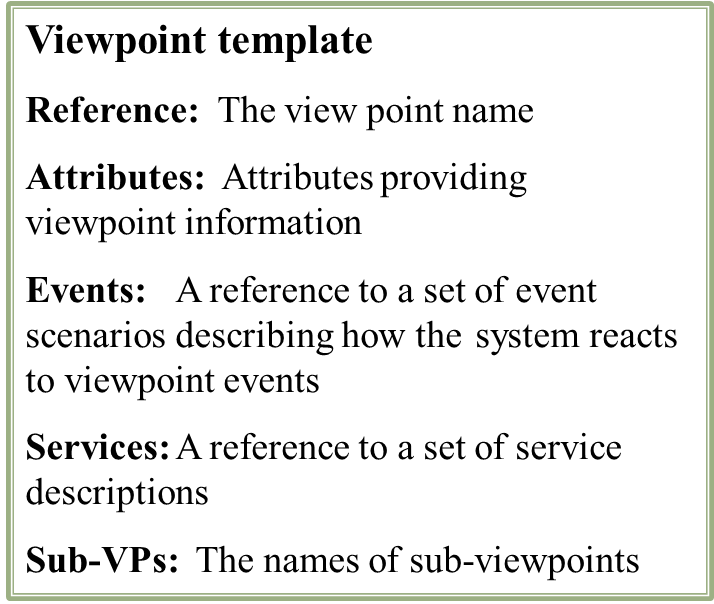
\includegraphics{Forelesning 08/img/2.png}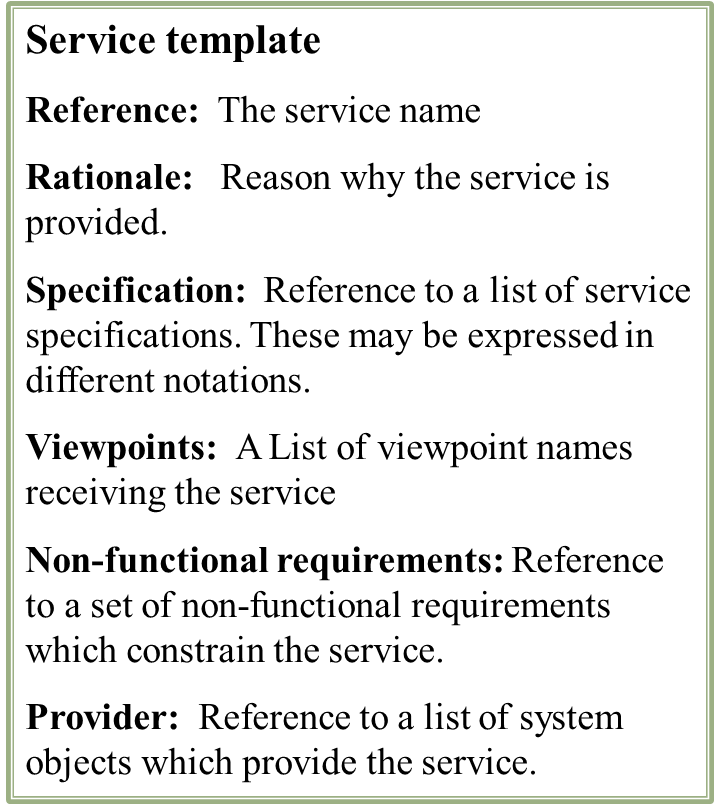
\includegraphics{Forelesning 08/img/3.png}
Et eksempel med kunde (customer) og skal ta ut penger (cash withdrawal)
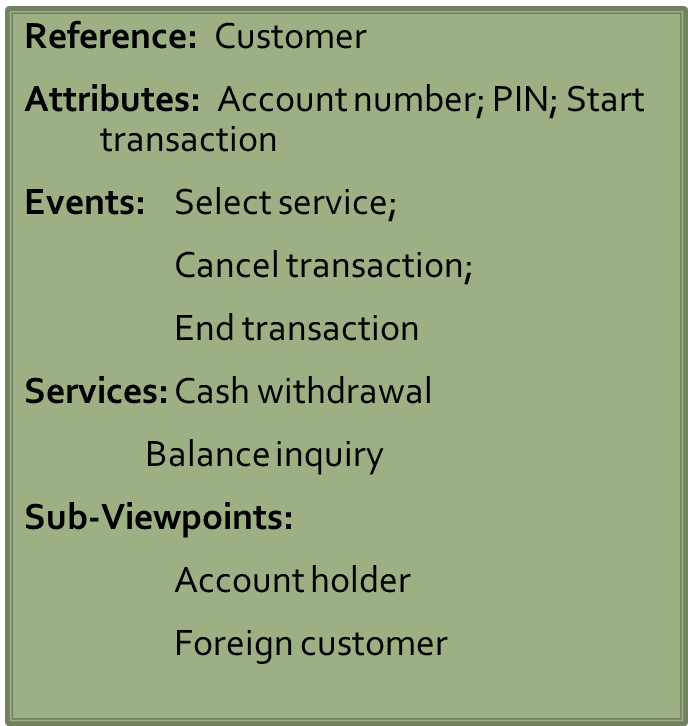
\includegraphics{Forelesning 08/img/4.png}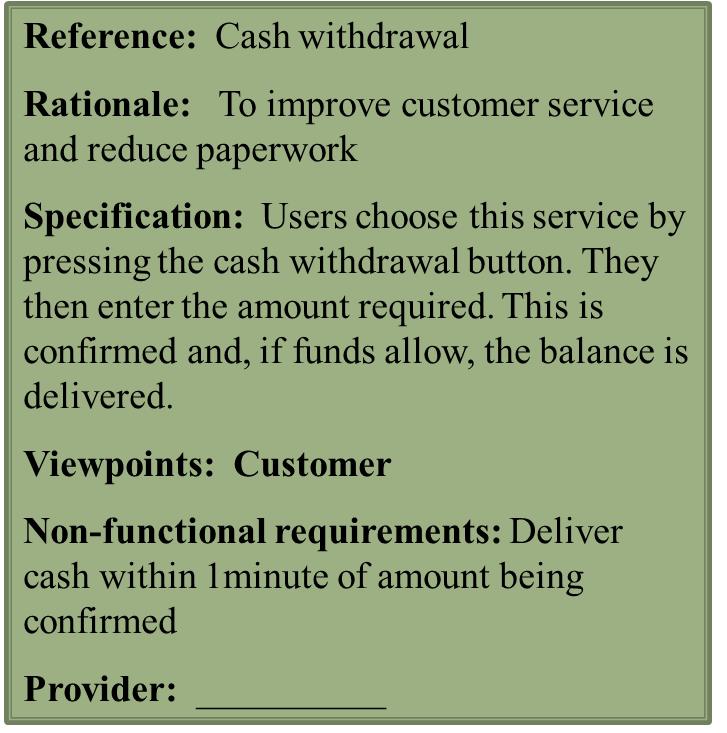
\includegraphics{Forelesning 08/img/5.png}

\subsection{Kravhåndtering - Viewpoint}

\subsubsection{Fordeler med viewpoint-orientert tilnærming i
kravhåndtering}

\begin{itemize}
\item
  Assisterer med å forstå og kontrollere kompleksiteten ved å separere
  interessene til de ulike aktørene
\item
  Eksplisitt gjenkjenne mangfoldet det er av kilder til krav
\item
  Gir en mekanisme for å organisere og strukturere dette mangfoldet
\item
  Får en slags fullstendighet
\item
  Gir mulighet for kravkildene eller stakeholders til å identifisere og
  sjekke deres bidrag til kravene.
\end{itemize}
\subsubsection{Non functional requirement}

Et mål er oppnådd når alle dets delmål er oppnådd. NFR Framework er
sentrert rundt såkalte soft goals, som ikke har noe klart kritere for
oppnåelse. Slike soft goals er oppnådd når det er nok positive og lite
negative bevis for målet og vice-versa når det er mye negativt og lite
positivt. Soft goals analyseres i relasjon med hverandre.

\paragraph{Non functional requirement Framework (NFRF):}

Analyse for ikke-funksjonelle krav:

\begin{enumerate}[1.]
\item
  Starter med soft goals som representerer ikke-funksjonelle mål. Disse
  er interessentene blitt enige om, f.eks usability, flexibility etc.
\item
  Hvert soft goal refineres så ved å bruke dekomposisjon.
\end{enumerate}
Dekomposisjon kan baseres på : Generell ekspertise rundt f.eks security,
flexibility. Domene-spesifikk kunnskap. Prosjekt-spesifikk kunnskap. Se
foilene for eksempel på NFR-analyse/-dekomposisjon.

Fordeler ved NFR rammeverket: NFR oppnås ved å samle kunnskap om domenet
for et system skal bygges. NFRF fokuserer på å klargjøre meningen til de
ikke-funksjonelle kravene. NFRF gir alternativer for oppfyllelse av soft
goals.

\subsubsection{Cross cutting (tverrgående) krav:}

Et delmål, et konkret krav kan være involvert i oppfyllingen til flere
enn et høynivå-mål. Mange ikke-funksjonelle krav faller i denne
kategorien. F.eks : Ytelse er en faktor av systemarkitekturen. Vi kan
ikke utvikle en ytelsesmodul som er uavhengig av de andre delene til
systemet. Det er slike krav som kalles tverrgående krav. Eksempler på
slike er : Sikkerhet, mobilitet, tilgjengelighet og
sanntidsbegrensninger.

\paragraph{Aspekt-orientert requirement engineering}

Handler om å identifisere tverrgående krav tidlig i krav og
arkitekturdesign fasen, istedet for i implementasjonsfasen. 4 steg :
Identifisere, fange (capture), komponere (compose) og analysere. Se
foiler for dyptgående eksempel av et banksystem med tverrgående krav.
Her prøver man å skrive om krav for å fjerne spredte konsepter.

\subsubsection{COTS (Commercial off the shelf)}

Når størrelsen og kompleksiteten til systemer vokser, ser man på COTS
som en mulig løsning. Her blir krav begrenset av tilgjengeligheten til
passende COTS-komponenter. Viktig aspekt er å evaluere mulig COTS
programvare tidlig i livssykelen til prosjektet.

\emph{Impact av COTS :} For bedriftsapplikasjoner kan man bruke et stort
COTS-produkt til å levere et eller flere krav (f.eks MS Office eller
Oracle) For innebygde sanntids- eller sikkerhetskritiske domener, er
COTS forventet å være små, og kreve store mengder av ``lim-kode'' til å
integrere COTS komponentene med resten av systemet.

\emph{Problemer med COTS:}

\begin{itemize}
\item
  Begrenset tilgang til produktets interne design
\item
  Beskrivelsen av kommersielle pakker er noen ganger ufullstendig og
  forvirrende
\item
  Kunder har en begrenset sjanse til å verifisere hvorvidt et ønsket
  krav er møtt.
\item
  De fleste av seleksjonsavgjørelsene er basert på subjektivitet, slik
  som partnerskap og markedsføring.
\end{itemize}
\emph{Fordeler med COTS:} vi får et produkt som har blitt testet mange
ganger av ekte brukere med konsekvent forbedring av
programvarekvaliteten. Se foil 8.2 (Requirements) for eksempel på
COTS-krav.

\subsubsection{Krav for outsourcing}

Outsourcing er en management strategi, hvor en organisasjon outsourcer
store, ikke-kjernefunksjoner til tjenestetilbydere og tredjeparter.
Outsourcing blir stadig mer vanlig. Skiller mellom:

\begin{itemize}
\item
  Onshore : Outsource et prosjekt innad i eget land
\item
  Offshore : Outsource til land utenfor europa (f.eks India)
\item
  Nearshore : Nearshore vil for Norge og Skandinavia være baltiske land
  (ikke lange avstander)
\end{itemize}
\paragraph{Faser i outsourcing:}

\emph{Seleksjon} : Velge underleverandør. \emph{Monitoring} : Signere
kontrakte og følge underleverandørens arbeid til produktet er levert.
\emph{Fullføring} : Akseptanse og installering av produktet, og også
vedlikehold av produktet i dets levetid.

\paragraph{Fordeler og ulemper}

\emph{Fordeler:} Kostnadsbesparende. Bedre tjenestelevering og kvalitet.
Holde tritt med teknologisk innovasjon. \emph{Ulemper:} Firmaer mister
kontroll over business-processes og inhouse ekspertise.

\subsection{Konklusjon}

Flere måter å identifisere og behandle krav på, hver med sine iboende
kompleksiteter og avhengigheter. Viewpoints prøver å eksplisitt
modellere interessene til de ulike aktørene. NFR-rammeverk fokuserer på
å modellere soft goals og klargjøre deres mening. Tidlige aspekter
fokuserer på å identifisere tverrgående forhold i krav i en tidlig fase
av prosjektet. Finnes ytterligere kravbehandlingshensyn når man bruker
COTS eller outsourcer.

\section{8.1 - Test-prioritering}

Selv om der er mange måter å prioritere tester på vil dette kurset
fokusere mest på \emph{risikobasert prioritering}. Nøkkelord er:
\emph{risikovurdering} (assessment) og \emph{prioriteringsmekanismer}.

Riskikobasert testing er ikke et nytt fenomen, risikovurdering har blitt
brukt lenge av selskaper som utvikler programvare. Dette har dog skjedd
på en ustrukturert måte, uten nødvendig dokumentasjon. Vi behøver
systematiske metoder for å best kunne håndtere denne risikoanalysen og
utføre risikobasert testing.

Risko er et \emph{forhold mellom et system og dets miljø}. Derfor vil en
risiko, dens hyppighet og viktighet variere med interessentene.
Sannsynligheten for at den vil oppstå en systemkarakteristikk, men
konsekvenser av den vil allikevel variere. Første steg er derfor å
identifisere og analysere interessentene.

\subsection{Interessenter (Stakeholders)}

De to hovedgruppene interessenter er \emph{kunder} og \emph{selskapet}.
Kunder vil kunne miste penger, enten direkte eller indirekte (på grunn
av feilen vil en kunne miste forretninger). Selskapet vil og kunne miste
penger via tap av troverdighet. Det er derfor svært viktig at alle
interessenter er involverte i risikovurderinger. De vil ha ulik
ekspertise og erfaring, som kan bidra til et bedre, bredere
datagrunnlag. Videre, grunnet den ulike erfaringen til interessentene må
metodene som benyttes for vurderigen være både \emph{enkle i bruk}
(helst skal en ikke behøve opplæring i metodene) og \emph{enkle å
forstå} (mennesker har lite tillit til ting de ikke forstår).

\subsection{Risikoidentifikasjon}

Det en starter med når en skal identifisere relevante risiko er
systemets definerte \emph{use cases}. Hver av deltakerne må derfor på
forhånd gjøre seg kjente med disse diagrammene. Det er og lurt med en
oppvarmingsøvelse for å utslette misforståelser og å bli enige om en
felles prosess. En slik øvelse kan være å gå gjennom resultatene fra
tidligere risikoidentifikasjonsprosesser.

I løpet av risikoidentifikasjonsprosess søker en svar på følgende
spørsmål for hver enkelt funksjon:

\begin{itemize}
\item
  Hvordan kan denne funksjonen feile?
\item
  Hva er sannsynligheten for at det eksisterer defekter i denne delen av
  koden?
\item
  Hvilke konsekvenser har disse feilene for interessentene?
\end{itemize}
Videre vil en kartlegge alvorligheten av hver enkelt feil-modus, og
dokumentere resultater fra prosessen i en konsekvenstabell.

\ctable[pos = H, center, botcap]{llllll}
{% notes
}
{% rows
\FL
\parbox[b]{0.22\columnwidth}{\raggedright
\emph{Function}
} & \parbox[b]{0.22\columnwidth}{\raggedright
\emph{Failure mode descripton}
} & \parbox[b]{0.41\columnwidth}{\raggedright
\emph{Code involved}
} & \parbox[b]{0.05\columnwidth}{\raggedright
\emph{User}
} & \parbox[b]{0.05\columnwidth}{\raggedright
\emph{Cust.}
} & \parbox[b]{0.05\columnwidth}{\raggedright
\emph{Dev.}
}
\ML
\parbox[t]{0.22\columnwidth}{\raggedright
Hva brukeren ønsker å oppnå.
} & \parbox[t]{0.22\columnwidth}{\raggedright
Hvordan funksjonen kan feile.
} & \parbox[t]{0.41\columnwidth}{\raggedright
Systemelementer involvert. Hvor sannsynlig er det at feilen vil
forårsake feilmodus.
} & \parbox[t]{0.05\columnwidth}{\raggedright
} & \parbox[t]{0.05\columnwidth}{\raggedright
} & \parbox[t]{0.05\columnwidth}{\raggedright
}
\LL
}

\subsection{Risikovurdering}

For å være nyttig må en risikovurdering være basert på relevant
erfaring, være ankret i den virkelige verden, og være et resultat av en
dokumentert og \emph{agreed-upon} prosess. En risikovurdering er en
subjektiv prosess, men det er svært viktig å ha et solid datagrunnlag
for de tall og prognoser som prosessen resulterer i.

Spørsmål som besvares gjennom en slik prosess er gjerne spørsmål som:

\begin{itemize}
\item
  Kan dette virkelig skje? Har det samme eller noe lignende skjedd før?
\item
  Kan vi forklare en plausibel årsak? Kan vi identifisere en
  konsekvenskjede for hendelsen?
\item
  Hvor ille kan det bli?
\item
  Hvor ofte har dette skjedd før?
\end{itemize}
\subsection{Hvordan gjøre en risikovurdering}

Overordnet er det det to måter å gjøre risikovurderinger:
\emph{kvantitativt} og \emph{kvalitativt}. Kvalitative vurderinger
gjøres enten via en \emph{sannsynlighet-/konsekvens-matrise} og via
\emph{GALE} (Global At Least Equivalent) -metoden. Kvantitativ vurdering
gjøres med \emph{CORAS-modellen}.

\subsubsection{Kvalitativ vurdering}

Når en utfører kvalitativ vurdering benytter en seg av skalaer. Disse må
en selv bestemme seg for på forhånd -- en skala fra 1 til 10 er like
``riktig'' som lav-middels-høy-type kategorier.

\paragraph{Kategorier}

Når en benytter seg av kategorier er det svært viktig å gi en kort
beskrivelse av hva hver enkelt kategori impliserer. Dette gjøres ved å
relatere det til noe kjent, det vil si for eksempel prosjektets
størrelse, selskapets turn-over og/eller selskapets profitt. Et eksempel
på dette er for konsekvenser si at kategorien \textbf{høy} vil bli gitt
konsekvenser som på en alvorlig måte setter prosjektets lønnsomhet i
fare. I tilfellet for sannsynlighet kan en si at \textbf{lav} betyr at
hendelsen \emph{kan} intreffe, men bare i ekstreme tilfeller.

Produktet av \texttt{konsekvens * sannsynlighet} brukes for å videre
bestemme viktigheten av en risiko. En generell regel er at en kun vil se
på de risikoer over en gitt sperregrense (M eller L).

\paragraph{GALE-modellen}

GALE-modellen er en metode som brukes for beslutningstaking hvor en vil
bestemme seg for om hvorvidt en forandring skal introduseres eller ei.
Modellen er noe mer komplisert enn den versjonen som benyttes i dette
kurset, hvor kun risikovurderingsskjemaet benyttes. Dette skjemaet
fokuserer på avvik fra nåværende gjennomsnitt.

GALE-indeksen regnes ut på bruk av vurdering av en hendelses
\emph{frekvens}, \emph{sannsynligheten} for at en oppstått hendelse skal
forårsake problemer og hendelsens \emph{alvorlighet}. Risikoindeksen er
definert som \texttt{I = Fe + Pe + S}.

\subparagraph{Frekvens-score for en hendelse}

\ctable[pos = H, center, botcap]{lrll}
{% notes
}
{% rows
\FL
\parbox[b]{0.24\columnwidth}{\raggedright
\emph{Frekvensklasse}
} & \parbox[b]{0.15\columnwidth}{\raggedleft
\textbar{}
} & \parbox[b]{0.54\columnwidth}{\raggedright
\emph{Hendelser per prosjekt}
} & \parbox[b]{0.07\columnwidth}{\raggedright
\emph{Fe}
}
\ML
\parbox[t]{0.24\columnwidth}{\raggedright
Veldig Ofte
} & \parbox[t]{0.15\columnwidth}{\raggedleft
200 \textbar{}
} & \parbox[t]{0.54\columnwidth}{\raggedright
Hvert prosjekt
} & \parbox[t]{0.07\columnwidth}{\raggedright
6
}
\\\noalign{\medskip}
\parbox[t]{0.24\columnwidth}{\raggedright
Ofte
} & \parbox[t]{0.15\columnwidth}{\raggedleft
100 \textbar{}
} & \parbox[t]{0.54\columnwidth}{\raggedright
Et prosjekt i blant
} & \parbox[t]{0.07\columnwidth}{\raggedright
5
}
\\\noalign{\medskip}
\parbox[t]{0.24\columnwidth}{\raggedright
Sannsynlig
} & \parbox[t]{0.15\columnwidth}{\raggedleft
40 \textbar{}
} & \parbox[t]{0.54\columnwidth}{\raggedright
Hvert 10. prosjekt
} & \parbox[t]{0.07\columnwidth}{\raggedright
4
}
\\\noalign{\medskip}
\parbox[t]{0.24\columnwidth}{\raggedright
Av og til
} & \parbox[t]{0.15\columnwidth}{\raggedleft
10 \textbar{}
} & \parbox[t]{0.54\columnwidth}{\raggedright
Hvert 100. prosjekt
} & \parbox[t]{0.07\columnwidth}{\raggedright
3
}
\\\noalign{\medskip}
\parbox[t]{0.24\columnwidth}{\raggedright
Sjeldent
} & \parbox[t]{0.15\columnwidth}{\raggedleft
1 \textbar{}
} & \parbox[t]{0.54\columnwidth}{\raggedright
Noen få ganger i selskapets levetid
} & \parbox[t]{0.07\columnwidth}{\raggedright
2
}
\\\noalign{\medskip}
\parbox[t]{0.24\columnwidth}{\raggedright
Usannsynlig
} & \parbox[t]{0.15\columnwidth}{\raggedleft
0,2 \textbar{}
} & \parbox[t]{0.54\columnwidth}{\raggedright
En eller to ganger i selskapets levetid
} & \parbox[t]{0.07\columnwidth}{\raggedright
1
}
\\\noalign{\medskip}
\parbox[t]{0.24\columnwidth}{\raggedright
Utrolig
} & \parbox[t]{0.15\columnwidth}{\raggedleft
0,01 \textbar{}
} & \parbox[t]{0.54\columnwidth}{\raggedright
En gang i selskapets levetid
} & \parbox[t]{0.07\columnwidth}{\raggedright
0
}
\LL
}

\subparagraph{Sannsynlighetsscore for en hendelse}

\ctable[pos = H, center, botcap]{lll}
{% notes
}
{% rows
\FL
\parbox[b]{0.18\columnwidth}{\raggedright
\emph{Klassifisering}
} & \parbox[b]{0.77\columnwidth}{\raggedright
\emph{Interpretasjon}
} & \parbox[b]{0.05\columnwidth}{\raggedright
\emph{Pe}
}
\ML
\parbox[t]{0.18\columnwidth}{\raggedright
Sannsynlig
} & \parbox[t]{0.77\columnwidth}{\raggedright
Det er sannsynlig at hendelsen, dersom den oppstår, vil føre til et
problem.
} & \parbox[t]{0.05\columnwidth}{\raggedright
3
}
\\\noalign{\medskip}
\parbox[t]{0.18\columnwidth}{\raggedright
Av og til
} & \parbox[t]{0.77\columnwidth}{\raggedright
Hendelsen, dersom den oppstår, vil av og til føre til et problem.
} & \parbox[t]{0.05\columnwidth}{\raggedright
2
}
\\\noalign{\medskip}
\parbox[t]{0.18\columnwidth}{\raggedright
Sjeldent
} & \parbox[t]{0.77\columnwidth}{\raggedright
Det er en liten sjanse for at hendelsen, dersom den oppstår, vil føre
til et problem.
} & \parbox[t]{0.05\columnwidth}{\raggedright
1
}
\\\noalign{\medskip}
\parbox[t]{0.18\columnwidth}{\raggedright
Usannsynlig
} & \parbox[t]{0.77\columnwidth}{\raggedright
Det er usannsynlig at hendelsen, dersom den oppstår, vil føre til et
problem.
} & \parbox[t]{0.05\columnwidth}{\raggedright
0
}
\LL
}

\subparagraph{Alvorlighetsscore for en hendelse}

\ctable[pos = H, center, botcap]{lll}
{% notes
}
{% rows
\FL
\parbox[b]{0.19\columnwidth}{\raggedright
\emph{Alvorlighetsklasse}
} & \parbox[b]{0.76\columnwidth}{\raggedright
\emph{Interpretasjon}
} & \parbox[b]{0.05\columnwidth}{\raggedright
\emph{S}
}
\ML
\parbox[t]{0.19\columnwidth}{\raggedright
Alvorlig
} & \parbox[t]{0.76\columnwidth}{\raggedright
Andelen forekommede problemer har alvorlige konsekvenser i mye større
grad enn gjennomsnittlig.
} & \parbox[t]{0.05\columnwidth}{\raggedright
2
}
\\\noalign{\medskip}
\parbox[t]{0.19\columnwidth}{\raggedright
Gjennomsnittlig
} & \parbox[t]{0.76\columnwidth}{\raggedright
Andelen forekommede problemer har alvorlige konsekvenser i en
gjennomsnittlig grad.
} & \parbox[t]{0.05\columnwidth}{\raggedright
1
}
\\\noalign{\medskip}
\parbox[t]{0.19\columnwidth}{\raggedright
Små
} & \parbox[t]{0.76\columnwidth}{\raggedright
Andelen forekommede problemer har alvorlige konsekvenser i mye mindre
grad enn gjennomsnittlig.
} & \parbox[t]{0.05\columnwidth}{\raggedright
0
}
\LL
}

\subsubsection{CORAS-modellen}

CORAS er utviklet som et rammeverk for det å vurdere sikkerhetsrisiko.
Det som er av viktighet her er hvordan CORAS relaterer seg til
kvalitative riskokategorier som omhandler selskapets turn-over.

Da det er vanskelig å finne realistiske verdier for alle risiko og at
det ikke alltid er innlysende hvordan en sammenligner kvalitative og
kvantitative risiko, er verdien av kvantitative risiko og muligheter
begrenset, selv om de tilbyr håndfaste verdier. Ved bruk av
CORAS-tabeller er det svært viktig å huske at utviklere, kunder og
brukere vil ha ulike verdier på de ulike postene, da en har ulike
utgangspunkt for det å verdsette disse.

\begin{figure}[htbp]
\centering
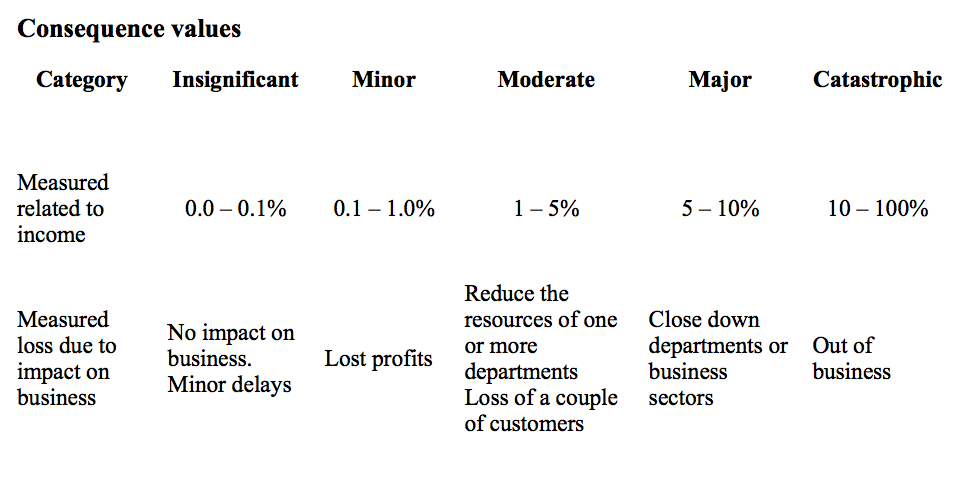
\includegraphics{Forelesning 08/img/coras.png}
\caption{}
\end{figure}

Det er mulig å forstå frekvenser på to måter: målt i antall uønskede
hendelser per år; og andel feilende etterspørringer/leveringer.

CORAS frekvens-tabell

\ctable[pos = H, center, botcap]{llllll}
{% notes
}
{% rows
\FL
\parbox[b]{0.23\columnwidth}{\raggedright
\emph{Kategori}
} & \parbox[b]{0.17\columnwidth}{\raggedright
\emph{Sjeldent}
} & \parbox[b]{0.19\columnwidth}{\raggedright
\emph{Usannsynlig}
} & \parbox[b]{0.17\columnwidth}{\raggedright
\emph{Mulig}
} & \parbox[b]{0.17\columnwidth}{\raggedright
\emph{Sannsynlig}
} & \parbox[b]{0.07\columnwidth}{\raggedright
\emph{Svært trolig}
}
\ML
\parbox[t]{0.23\columnwidth}{\raggedright
Antall uønskede hendelser per år
} & \parbox[t]{0.17\columnwidth}{\raggedright
1/100
} & \parbox[t]{0.19\columnwidth}{\raggedright
1/100 - 1/50
} & \parbox[t]{0.17\columnwidth}{\raggedright
1/50 - 1
} & \parbox[t]{0.17\columnwidth}{\raggedright
1 -12
} & \parbox[t]{0.07\columnwidth}{\raggedright
\textgreater{} 12
}
\\\noalign{\medskip}
\parbox[t]{0.23\columnwidth}{\raggedright
Antall uønskede hendelser per etterspørring
} & \parbox[t]{0.17\columnwidth}{\raggedright
1/1000
} & \parbox[t]{0.19\columnwidth}{\raggedright
1/500
} & \parbox[t]{0.17\columnwidth}{\raggedright
1/50
} & \parbox[t]{0.17\columnwidth}{\raggedright
1/25
} & \parbox[t]{0.07\columnwidth}{\raggedright
1/1
}
\\\noalign{\medskip}
\parbox[t]{0.23\columnwidth}{\raggedright
Interpretasjon av antall etterspørringer
} & \parbox[t]{0.17\columnwidth}{\raggedright
Uønskede hendelser skjer aldri.
} & \parbox[t]{0.19\columnwidth}{\raggedright
Hvert tusende gang systemet brukes.
} & \parbox[t]{0.17\columnwidth}{\raggedright
Hver femte gang systemet brukes.
} & \parbox[t]{0.17\columnwidth}{\raggedright
Hver tiende gang systemet brukes.
} & \parbox[t]{0.07\columnwidth}{\raggedright
Hver gang systemet brukes.
}
\LL
}

\paragraph{Eksempel}

Under er et eksempel på bruk.

\ctable[pos = H, center, botcap]{ll}
{% notes
}
{% rows
\FL
\parbox[b]{0.28\columnwidth}{\raggedright
Tekst
} & \parbox[b]{0.44\columnwidth}{\raggedright
Tall
}
\ML
\parbox[t]{0.28\columnwidth}{\raggedright
\emph{Årlig intekt}
} & \parbox[t]{0.44\columnwidth}{\raggedright
100.000.000
}
\\\noalign{\medskip}
\parbox[t]{0.28\columnwidth}{\raggedright
\emph{Feilkonsekvens}
} & \parbox[t]{0.44\columnwidth}{\raggedright
0.001 - 0.01 (mindre)
}
\\\noalign{\medskip}
\parbox[t]{0.28\columnwidth}{\raggedright
\emph{Feilfrekvens}
} & \parbox[t]{0.44\columnwidth}{\raggedright
1 per år - 2 per 100 år (mulig)
}
\LL
}

\texttt{maksimal risiko = 100.000.000 * 0.01 * 1 = NOK 1.000.000}

\texttt{minimal risiko = 100.000.000 * 0.001 * 1/50 = NOK 2.000}

\subsection{Worry List}

Testing er en ``sampling''-prosess, noe som vil si at dersom vi finner
mange defekter i en komponent bør vi konkludere med at komponenten har
mange defekter. Denne konklusjonen vil ikke nødvendigvis være den samme
hvis vi baserer konklusjonen på antallet defekter funnet i en
inspeksjon.

\begin{figure}[htbp]
\centering
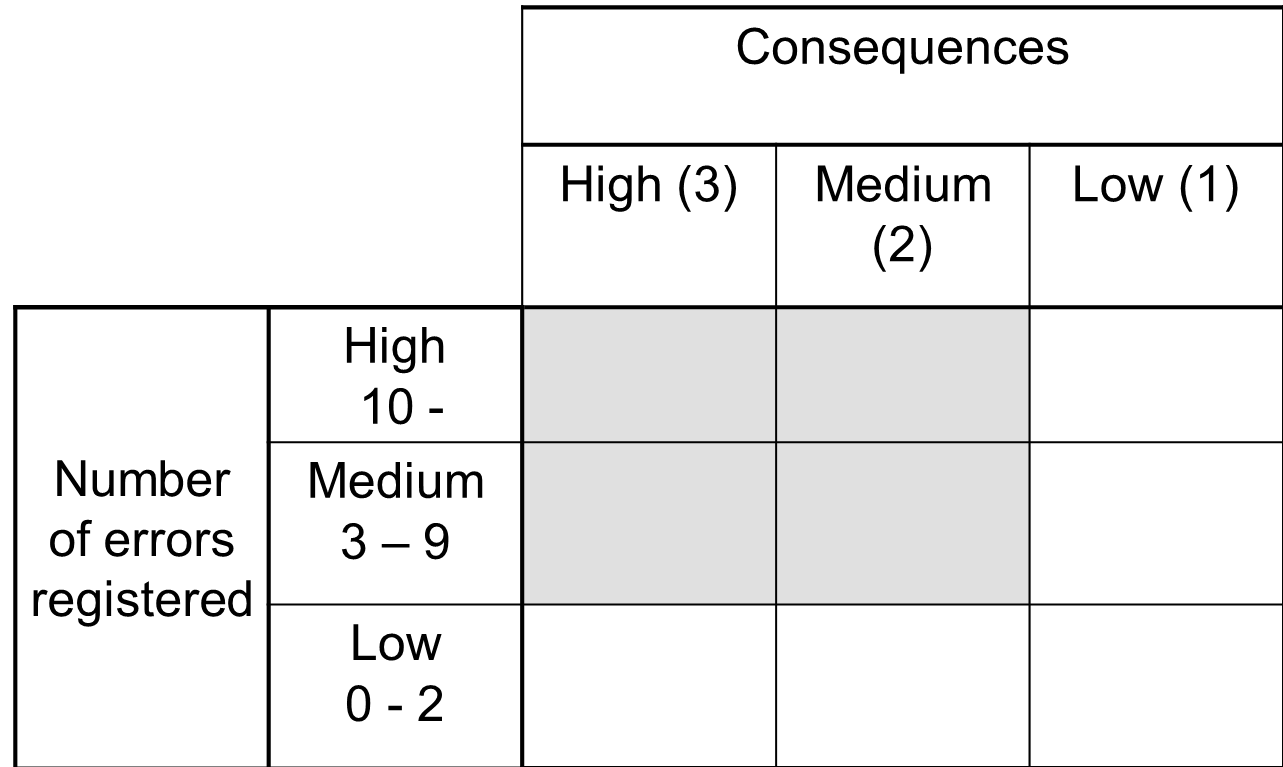
\includegraphics{Forelesning 08/img/1.png}
\caption{Testcase for alfa -\textgreater{} A -\textgreater{} C
-\textgreater{} A:}
\end{figure}

\subsection{Risikobasert testing}

Risikobasert testing involverer følgende to steg:

\begin{enumerate}[1.]
\item
  Identifisere hvordan produktet interagerer med sitt miljø. Dette
  gjøres for å \emph{forstå konsekvenser av feil}.
\item
  Identifisere og rangere risiko etter sannsynlighet og konsekvens.
  \begin{itemize}
  \item
    Dersom det er en white box- eller grey box-test bør en også
    identifisere mulige kausale hendelseskjeder med den hensikt å forstå
    feilmekanismene.
  \end{itemize}
\item
  Definere tester som kan brukes for å forsikre at sannsynligheter for
  defekter i koden er lav.
  \begin{itemize}
  \item
    Black box-testing -- tilfeldig testing eller domenetesting
  \item
    White box- eller grey box-testing -- forsikre at alle identifiserte
    kausale hendelesforløp benyttes og testes skikkelig.
  \end{itemize}
\item
  Kjøre testene. En starter med de høyeste risikoer og jobber seg
  nedover.
\end{enumerate}
\subsection{Eksempel på bruk av ATM}

\begin{figure}[htbp]
\centering
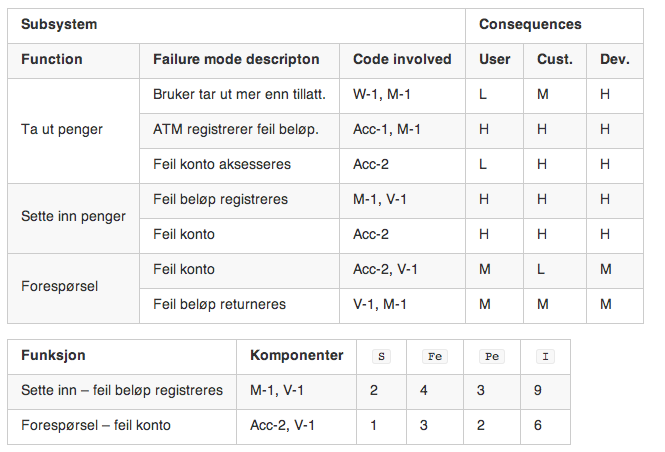
\includegraphics{Forelesning 08/img/ATM-ex.png}
\caption{}
\end{figure}

\section{15.1 - Regresjonstesting}

Regresjonstesting er testing gjort for å kontrollere at en
systemoppdatering ikke reintroduserer feil som har blitt fikset
tidligere. Dette gjøres via black-box-testing (for å teste
funksjonalitet) og grey-box-testing (for å teste arktitekturen).

Ettersom regresjonstester er ment å teste all funksjonalitet og alle
forandringer, vil slike tester være store. Av den grunn må
regresjonstesting eksekveres og kontrolleres automatisk.

\subsection{Automatisk regresjonstesting}

Parameterisering av testresultater. I stedet for å bruke en komplett
output-fil som orakel vil vi bruke et verktøy for å ekstrahere
\emph{relevant} data fra filen. Disse dataene vil vi så bruke sammen med
de data som er lagret i orakelet.

Da en regresjonstest er stor vil det alltid være et behov for å
identifisere de deler av en regresjonstest som behøves å kjøre etter en
forandring. Traceability er derfor viktig av to grunner: mindre
eksekveringstid; vite hvilke tester som må forandres når funksjonalitet
endres.

Implementerte regresjonstester må holdes oppdatert hver gang koden
oppdateres. Skapes det varianter av systemet må der også skapes
parallelle varianter av regresjonstest-suiten.

\subsection{Bug fixing}

\begin{enumerate}[1.]
\item
  Rapportering av bug
\item
  Reprodusering av bug, helst med en så enkel input-sekvens som mulig
\item
  Lag en ny oppføring i regresjonstesten, sammen med
  \begin{itemize}
  \item
    Rapportert inputsekvens (realistisk, men kan være stor)
  \item
    Enklest mulig inputsekvens (enkel å forstå, men er kunstig)
  \end{itemize}
\end{enumerate}
\section{15.3 - Ikke-funksjonelle krav}

Standardisert i ISO-9126 (og mange andre steder) -- en
\emph{faktor-kriterie-metrikk-}modell. Nært koblet til ``quality in
use'' -- dvs. brukernes erfaring av systemet i bruk. Brukernes
erfaringer er subjektive og derfor vil og kvalitetsfaktorer være
subjektive.

\begin{figure}[htbp]
\centering
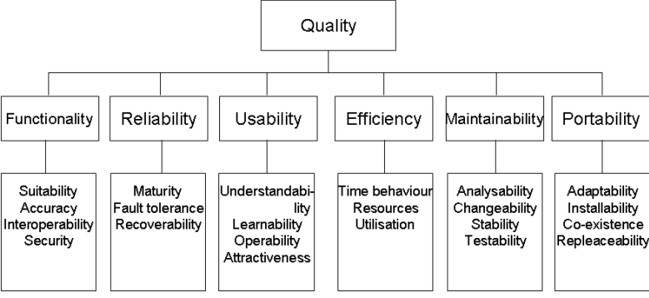
\includegraphics{Forelesning 15/img/quality.jpg}
\caption{Et nesten riktig diagram}
\end{figure}

\subsection{Functionality}

\begin{quote}
The capability of the software to provide functions which meet stated
and implied needs when the software is used under specified conditions.

\end{quote}
\subsubsection{Suitability}

Programvarens evne til å gi et hensiktsmessig sett funksjoner for
spesifiserte oppgaver og brukermål.

\subsubsection{Accuracy}

\ldots{}to provide the right or agreed.

\subsubsection{Interoperability}

Evne til å interagere med et eller flere spesifiserte systemer.

\subsubsection{Compliance}

Evne til å overholde applikasjonsrelaterte standarder, konvensjoner og
reguleringer i forhold til lover og forskrifter.

\subsubsection{Security}

Forhindre uønsket adgang, motstå angrep, uønskede modifikasjoner til
informasjon, gi angriper en mulighet til å forhindre adgang til legitme
brukere (DOS).

\subsection{Reliability}

\begin{quote}
The capability of the software to maintain the level of performance of
the system when used under specified conditions.

\end{quote}
Merk at slitasje og aldring ikke er med i denne beregningen, men kun
begrensninger gitt i kraft av mangler i krav, design og implementasjon.

\subsubsection{Maturity}

Unngå failure som et resultat av faults.

\subsubsection{Fault tolerance}

Opprettholde et spesifisert ytelsesnivå i tilfeller med store faults,
eller krenkelser av spesifisert grensesnitt.

\subsubsection{Recoverability}

Reetablering av ytelsesnivå, gjenopprette data rett etter failure.

\subsubsection{Availability}

Evne til å være i en fungerende tilstand til å utføre sine funksjoner på
et gitt tidspunk, under gitte bruksforhold.

\subsection{Usability}

\begin{quote}
The capability of the software to be understood, learned, used and liked
by the user, when used under specified conditions.

\end{quote}
\subsubsection{Understandability}

Gjøre en bruker i stand til å forstå om programvaren er passende og
hvordan den kan brukes for særlige oppgaver og bruksforhold.

\subsubsection{Learnability}

Gjør bruker i stand til å lære sin applikasjon.

\subsubsection{Operability}

Gjøre bruker i stand til å operere og kontrollere seg.

\subsubsection{Likeability}

Applikasjonens evne til å bli likt av en bruker.

\subsection{Efficiency}

\begin{quote}
The capability of the software to provide the required performance
relative to the amount of resources used, under stated conditions.

\end{quote}
\subsubsection{Time behaviour}

Gi hensiktsmessige respons- og prosesseringstider og throughput-rater
når den utfører sine funksjoner, under gitte forhold.

\subsubsection{Resource utilisation}

Bruke hensiktsmessige ressurser (annen programvare, HW, materialer) på
hensiktsmessig tidspunkt når den utfører sine funksjoner, under gitte
forhold.

\subsection{Maintainability}

\begin{quote}
The capability of the software to be modified (korrigeringer,
forbedringer, adapteringer).

\end{quote}
\subsubsection{Changeability}

Evne til å muliggjøre implementasjon av en spesifisert modifikasjon.

\subsubsection{Stability}

Minimisere ønskede bieffekter av modifikasjon. (ripple-effekt)

\subsubsection{Testability}

Muliggjøre testing av modifisert programvare.

\subsection{Portability}

\begin{quote}
The capability of software to be transferred from one environment
(organisational, HW, SW env) to another.

\end{quote}
\subsubsection{Adaptability}

Evne til å bli modifisert til et annet spesifisert mijø uten å gjøre noe
annet enn de handlinger som applikasjonen tillater.

\subsubsection{Installability}

Evne til å bli installert i et gitt miljø.

\subsubsection{Co-existence}

Evne til å sameksistere med annen uavhengig programvare i et felles
miljø med deling av felles ressurser.

\subsubsection{Conformance}

Evne til å overholde standarder og konvensjoner relatert til
portability.

\subsubsection{Replaceability}

Evne til å bli brukt i sted for annen spesifisert programvare dets
miljø.

\subsection{Setting av krav}

Minst tre måter:

\begin{itemize}
\item
  Brukernivå -- hvordan systemet oppfører seg
\item
  Posessnivå~-- hvordan produktet utvikles
\item
  Metrikknivå -- hvordan programvaren er
\end{itemize}
For å ha testbare kriterier må man gå ned på kriterienvå.

\subsubsection{MbO - Management by Objectives}

Starter med krav (systemet skal være enkelt å vedlikeholde). Spør så
\emph{``hva mener du med \ldots{}''} til du har noe observerbart og
testbart. I slike tilfeller må en ha en bruker som kan delta i testen på
en eller annen måte. Der vil nå være en sterk kobling mellom krav og
test -- i mange tilfeller vil kravet være testen.

Det er relativt enkelt å age krav som omhandler reliability,
maintainability og andre ``objektive'' ikke-funksjonelle krav på grunn
av at de er målbare. Subjektive faktorer som f.eks. usability er
vanskeligere. Men bruk MbO, skap tall der det er mulig (skal kunne læres
\textless{}1 uke).

Testen sier mer om kravet enn det kravet i seg selv sier.

\section{15.2 - Firewall for regresjonstesting}

Her brukes konseptet om en firewall for å redusere settet klasser eller
komponenter som behøves testes. Dette da de fleste regresjonsteseter er
store og tidkrevende.

En firewall i denne sammenhengen er en separator mellom de klasser som
beror på en klasse som endres fra resten.

Det finnes to sentrale konsepter,Dependency og encoding.

\subsection{Enkle regler for fire wall i et objektorientert system}

\begin{enumerate}[1.]
\item
  Gitt to suksessive versjoner av et objektorientert system, identifisér
  klasser som har blitt endret.
\item
  Dersom en klasse er en del av et arvshierarki må en også anse
  etterkommere av den endrede klassen som endret.
\item
  For hver endrede klasse, identifisér alle klasser som sender eller
  mottar meldinger til/fra den endrede klassen og inkludér de inne i
  firewallen.
\end{enumerate}
regel 4 og 5 identifiserer en utvidet fire wall

\begin{enumerate}[1.]
\setcounter{enumi}{3}
\item
  Identifisér alle datastier til og fra den endrede klassen
\item
  Finn alle eksterne klasser i den modifiserte klassens omfang og
  inkludér de i den utvidede firewallen
\end{enumerate}
\begin{figure}[htbp]
\centering
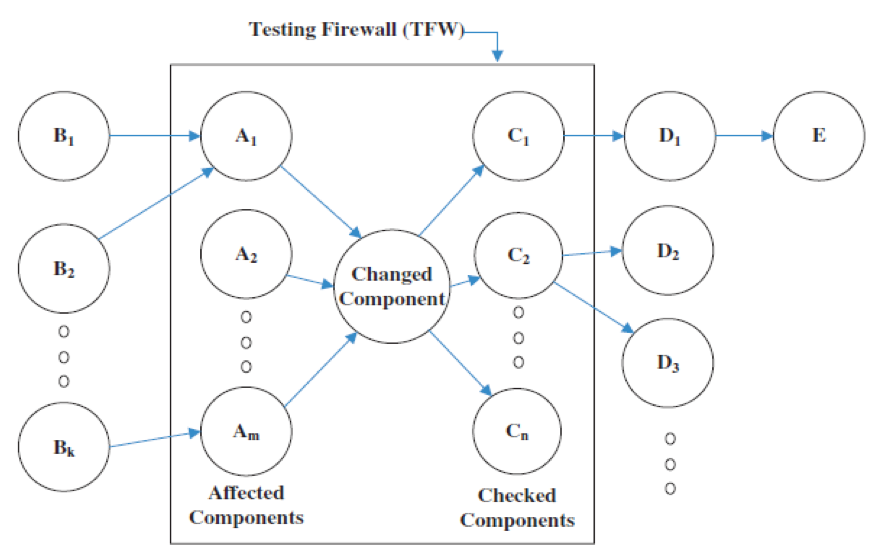
\includegraphics{Forelesning 15/img/firewall.png}
\caption{Testing firewall (TFW)}
\end{figure}

\subsection{Dependency}

To viktige spørsmål kommer opp her

\begin{enumerate}[1.]
\item
  Benytter komponenten seg vanlige verdier av inputen?
\item
  Må komponenten gjøre rede for hvordan denne inputen ble generert?
\end{enumerate}
Noen grunnregler for disse testee er at det bare skal bli brukt for å
teste oppdateringer og endringer. Det antas også at det innledende
testsettet og softwaren som er testet er av høy kvalitet.

IKKE FERDIG

\section{15.4 - Scenario testing}

Der finnes to typer scenariotesting, \emph{type 1} hvor scenarioer
benyttes for å definere input/output-sekvenser, og \emph{type 2} hvor
scenarioer brukes som et skript for sekvenser realistiske handlinger i
ekte eller simulerte omgivelser.

Mye av det en behøver for å skrive gode krav må brukes for å skrive gode
scenarioer. En av årsakene bak at scenario-testing er så effektivt kan
være at en i effekt går gjennom kravsprosessen nok en gang, men
involverer andre mennesker.

\subsubsection{Noen regler for å skrive gode scenarioer}

\begin{itemize}
\item
  List opp mulige brukere
  \begin{itemize}
  \item
    Analyse av mål og interesser
  \end{itemize}
\item
  List opp systemhendelser
  \begin{itemize}
  \item
    Definering/analyse av hvordan systemet håndterer dette
  \end{itemize}
\item
  List opp spesielle hendelser
  \begin{itemize}
  \item
    Hvordan imøtekommer systemet disse hendelsene?
  \end{itemize}
\item
  List opp nytte
  \begin{itemize}
  \item
    Lag en fremgangsmåte for hvordan en skal oppnå disse
  \end{itemize}
\item
  Jobb sammen med bruker
  \begin{itemize}
  \item
    Studér hvordan de arbeider, hva de gjør
  \end{itemize}
\item
  Les deg opp hva systemer av denne typen er ment å gjøre
\item
  Lag en liksomforretning
  \begin{itemize}
  \item
    Mat systemet med realistiske data.
  \end{itemize}
\end{itemize}
\subsection{Brukere}

De som vil bruke systemet som er under utvikling.

\subsubsection{List opp mulige brukere}

For hver identifiserte bruker - identifisér interesser. Fokusér på én
interesse om gangen og identifisér brukerens mål.

Finn så ut hvordan man best kan teste at hvert av målene er enkle å
oppnå med programvaren.

\subsubsection{List opp systemhendelser}

Hendelse : Enhvert tilfelle som systemet er ment å svare på.

For hver hendelse må vi forstå: dets \emph{formål}; hva systemet er ment
å gjøre med den; og regler relatert til hendelsen.

\subsubsection{List opp spesielle hendelser}

Forutsigbare, men uvanlige. Disse behøver spesiell håndtering.

Da disse behøver spesielle omstendigheter for å trigges må man sørge for
at scenarioene inkluderer de viktigste av disse omstendighetene.

\subsubsection{List opp nytte}

Hvilken nytte skal systemet gi brukerne? Dette må interessentene svare
på. Her er det viktig å passe på eventuelle misforståelser og
konflikter.

\subsubsection{Jobb sammen med bruker}

Det er svært viktig å jobbe sammen med systemets framtidige brukere. Her
kan en finne informasjon om hvordan de utfører sitt arbeide som gir en
pekere om hvordan systemet best kan oppfylle de må og ønsker en bruker
har. Se spesielt etter dagens arbeidsmønster og hva de har problemer
med.

Her vil en finne gode ideer til hvordan utforme scenarioer.

\subsubsection{Les om denne typen systemer}

Før en skriver scenarioer er det viktig å ha kunnskap om hva det nye
systemet skal gjøre, samt ha et innblikk i hva lignende systemer gjør.
Dette gir kunnskap om hva brukeren kan forvente av ens system. Denne
kunnskapen finner en gjerne i bøker, manualer, etc.

\subsubsection{Lag en liksomforretning}

Dette krever en god del kunnskap om hvordan forretningen fungerer. Det
er viktig at liksomforretningen er realistisk for å kunne få best mulig
resultat av øvelsen, og det kan være nødvendig å hente inn eksterne
konsulenter. Tar mye ressurser, men kan gi veldig verdifulle resultater.

\subsection{Risiko}

Passer ikke til testing av ny kode, da bugs i implementasjonen kan føre
til forsinkelser da testen må utsettes til disse er fikset. Derfor bør
scenariotesting kun brukes som en akseptansetest.

Scenarioer skal dekke alle systemets funksjonalteter, ikke kodedekning.
Avdekker designfeil heller enn kodefeil, og bør derfor ikke brukes den
til regresjonstesting, eller for testing av nye fixer.

\subsection{Type 1 scenariotesting}

Bruker scenarioer for a skrive transaksjoner som sekvenser av input og
forventet output. Resultatet kan være et ekstremt detljert tekstlig
usecase.

\subsection{Type 2 scenariotesting}

Brukes om en vil ha realisme. Her vil en teste hvordan systemet vil
oppføre seg i de real-world-situasjoner beskrevet av scenarioene, med
reelle brukere gitt av produkteier og (om nødvendig) med reelle kunder.

En type 2 scenariotest utføres på følgende måte:

\begin{enumerate}[1.]
\item
  Omgivelser settes opp i ifølge scenariobeskrivelsen. Kunder blir
  instruert i deres oppgaver.
\item
  En person -- game master -- leser hvert steg av scenarioene
\item
  Brukere og kunder reagerer på situasjonene GM skaper
\item
  Hendelsene som resulterer fra hvert scenario dokumenteres (f.eks. på
  video) for senere analyser
\end{enumerate}
Om der er for mange scenarioer (slik det ofte er), og en må prioritere
vil de scenarioer som involverer en sterk interaksjon med systemets
omgivelser (brukere, kunder, nettverk, filservere, stressende
arbeidssituasjon etc.) være de mest effektive.

\section{9.1 Outsourcing, subcontracting, COTS}

\subsection{Ansvar}

Viktig å tenke på:

\begin{itemize}
\item
  Firmaet som bringer produktet til markedet har fullt ansvar for
  produktets kvalitet
\item
  Er bare mulig å søke om oppreisning etter en outsourcing, dersom vi
  kan bevise at de ikke fullførte sin kontrakt.
\end{itemize}
\subsection{Testing og selvtillit}

Rollen testing har under:

\begin{itemize}
\item
  Utvikling - Finne og fjerne defekter
\item
  Akseptanse - Skape tillit til komponenten
\end{itemize}
Når vi tester COTS eller komponenter hvor utviklingen har blitt
outsourced/subcontracted, ønsker vi å skape tillit (confidence).

\subsubsection{Skape tillit til produktet:}

Man kan bygge tillit basert på : Produktet i seg selv, f.eks en COTS
komponent. Prosessen - hvordan den ble utviklet og testet. Folket -
personalet som har utviklet og testet komponenten.
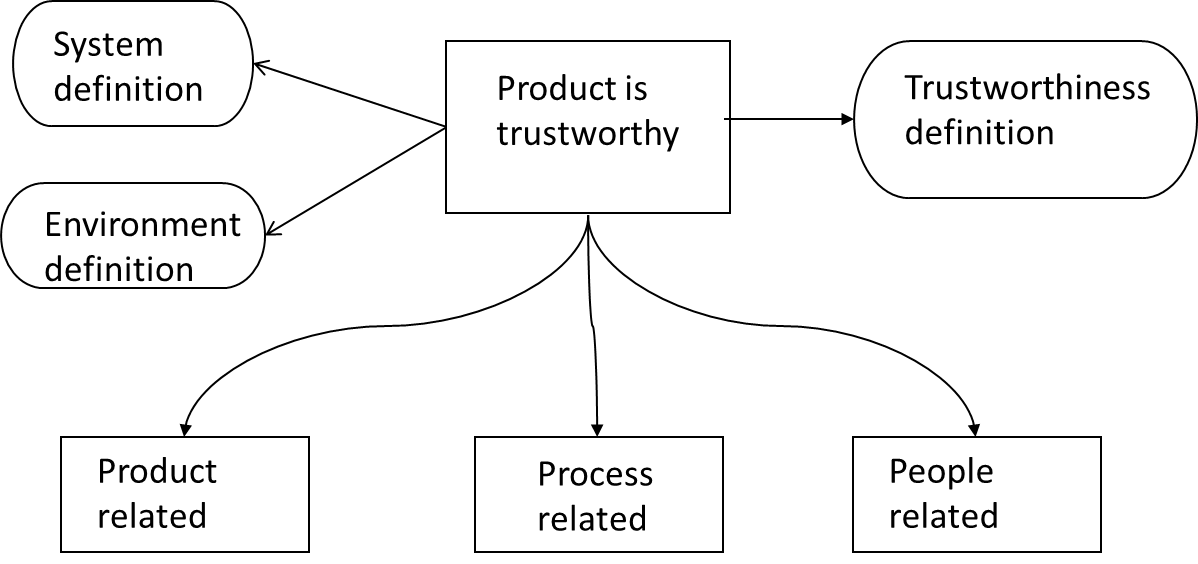
\includegraphics{Forelesning 09/img/2.png}

\subsubsection{Skape tillit til prosessen:}

Tillit i prosessen stammer fra tre kilder: Hvem gjør det? - ``Teamet er
kompetent'' . Hvordan blir det gjort? - ``Metoden adresserer
problemet''. Vi kan sjekke at prosessen blir brukt korrekt - ``Prosessen
er sporbar''.

\subsection{Testing og outsourcing}

Når vi outsourcer utvikling, må testingen være en integrert del av
utviklingsprosessen. Testing blir da altså et kontraktsspørsmål. Fra
trustworthiness-mønsteret ser vi at vi må inkludere krav for:
Komponenten - Hva . Kompetansen til personalet - Hvem . Prosessen -
Hvordan.

\subsubsection{Krav ved outsourcing.}

Når man skal tegne en outsourcing-kontrakt bør man inkludere:

\begin{itemize}
\item
  Krav til personell - riktige personer til jobben, se CV til hver
  person.
\item
  Utviklingsprosessen - inkludert testing. Slik tillit kan komme fra
  sertifikater(f.eks ISO 9001) eller egne prosessrevisjoner.
\item
  Prosjektplan - når skal de gjøre hva?
\item
  Teststrategi - Hvordan vil de teste komponentkravene våre?
\item
  Testplan - Hvordan vil testene bli kjørt?
\item
  Testlogg - hva var resultatet av testene?
\end{itemize}
\subsubsection{Tillit til komponenten}

Tilliten vi har til en komponent avhenger av hvor fornøyd vi er med
svarene på spørsmålene over. Vi kan dog også bygge tillit på tidligere
relasjoner med selskapet. Dess større denne tilliten basert på tidligere
erfaringer er, jo mindre strenge behøver vi være i kontrakten.

\subsection{Teste COTS}

COTS testes ved å benytte black-box testing eller
domene-partisjonstesting. Erfaringer tilsier at vi vil få mest utav
innsatsen ved å fokusere på tester for : Intern robusthet, og ekstern
robusthet.

\subsubsection{Robusthet}

\begin{itemize}
\item
  Intern Robusthet : Evnen til å behandle feil i komponenten eller dens
  miljø. Her trenger vi wrappers, feilinjeksjon etc. Her er komponenter
  som kun er synlige innenfor systemets grenser.
\item
  Ekstern robusthet : Evnen til å behandle feil input. Her trenger vi
  kun komponenten ``som den er''. Her er komponenter som er del av
  brukergrensesnittet.
\end{itemize}
Viktigheten av disse to typene vil variere, avhengig av typen
komponentener vi tester.

\paragraph{Intern robusthet}

Intern robusthet er evnen til å:

\begin{itemize}
\item
  Overleve alle feilaktige situasjoner som; Minnefeil - både kode og
  data. Feiling av funksjonskall, inkludert kall til OS-funksjoner.
\item
  Gå til en definert , \emph{trygg} tilstand etter å ha gitt
  feilmeldingen.
\item
  Fortsette etter en slik feilaktig situasjonen med et minimumstap av
  informasjon.
\end{itemize}
\paragraph{Wrappers}

En wrapper fungerer som en slags mellomtjener som gir oss et grensesnitt
hvor vi kan få tilgang til tjenester andre steder i systemet. Wrapperne
har som hovedoppgave å kalle andre klasser og metoder, gi oss tilgang
til disse gjennom et veldefinert grensesnitt uten å berøre andre deler.
Dette gir lavere kompleksitet. En wrapper har to essensielle
karakteristikker:

\begin{enumerate}[1.]
\item
  En implementasjon som definerer funksjonaliteten vi vil ha tilgang
  til. Dette kan være et objekt, men trenger ikke være det (Eksempel på
  ikke-objekt implementasjon: Vi trenger tilgang til funksjoner til en
  DLL).
\item
  ``Wrapper'' klassen gir oss tilgang til implementasjonen og metoder
  for å administrere implementasjonen. Klienten kaller en metode på
  wrapperen som igjen aksesserer implementasjonen som er nødvendig for å
  fullføre oppgaven.
\end{enumerate}
\emph{Hvorfor wrappers?} : Vi kontrollerer komponentens input, selv om
komponenten er i et ekte system. Vi kan samle og rapportere input og
output fra komponenten. Vi kan manipulere feilbehandlingen på denne ene
komponenten uten å berøre resten av systemet.

\paragraph{Fault injection}

En fault er en defekt eller unormal tilstand som kan føre til svikt i
systemet. Ved fault injection setter vi inn feil med vilje slik at vi
kan se responsen systemet gir. Målet er å ikke gjenskape omstendighetene
som fører til en slik feil. Fault injection brukes ofte med
stresstesting, og blir sett på som en viktig del av å utvikle robuste
systemer. To steg i fault injection:

\begin{enumerate}[1.]
\item
  Identifiser sett med feil som kan forekomme i et system, modul, klasse
  eller metode. Eksempel: Ikke noe vits å sette inn nettverksfeil dersom
  applikasjonen ikke bruker et nett.
\item
  Utøv disse feilene for å evaluere hvordan applikasjonen svarer. Typisk
  finner applikasjonen feilen, er feilen isolert og ``overlever''
  applikasjonen?
\end{enumerate}
Se foil 9-2 for utøvende eksempel på fault injection.

\paragraph{Ekstern robusthet}

Feilbehandling må bli testet for å vise at: Feil input gir en
feilmelding. Feilmeldingen skal være forståelig for de tenkte brukerne.
Systemet skal fortsette etter feilen med et minimalt informasjonstap.
Ekstern robusthet er evnen til å:

\begin{itemize}
\item
  Overleve input av feilaktig data (no crash)
\item
  Gi en enkel-å-forstå feilmelding som hjelper brukeren til å rette på
  inputfeil.
  \begin{itemize}
  \item
    Dette kan kun testes ved å involvere brukerne og er dermed ikke like
    lett å teste som de andre punktene. Vi trenger å vite hvilken info
    brukeren trenger for å kunne korrige feil i input og fortsette der
    han slapp i samme tilstand.
  \item
    Den enkleste måten å teste feilmeldinger på er å be en bruker om å
    begynne på en arbeidsoppgave, og sette inn en feil i input underveis
    i oppgaven. Vi kan da observere hvordan brukeren prøver å komme seg
    ut av situasjonen og hvor fornøyd han er med hjelpen han får fra
    systemet.
  \end{itemize}
\item
  Gå til en definert tilstand
\item
  Fortsette etter feilsituasjonen med et minimumstap av informasjon.
\end{itemize}
\paragraph{Sekvensiell testing}

Se foil for utøvende eksempel. P = target failure rate. hvis den er p
\textless{} 10\^{}3 så trenger man et stort antall tester. Det bør
derfor kun bli brukt for robusthettesting basert på automatisk generert
random-input Hvis p \textless{} 10\^{}1 , så vil sekvensiell testing gi
brukbare resultater selv om man inspiserer et forholdsvis stort antall
dokumenter.

\paragraph{Bayesian metoder}

Fremfor å bygge tillit kun på testresultater, kontrakter, eller
tidligere erfaring kan man kombinere disse tre faktorene, og dette
kalles bayesian statistikk.

Se foil 9-2 for dybtgående eksempel på bayes og sekvensiell testing med
bayes.

\section{9.2 - COTS-testing}

Ofte brukte tilnærminger til testing av COTS:

\begin{itemize}
\item
  Component meta-data
\item
  Retro-components (retrospector)
\item
  Built-in test (BIT)
\item
  STECC strategy
\item
  COTS
\end{itemize}
\subsection{Component meta-data}

Meta-data : Data relatert til komponenter, \emph{men er ikke kode}.

Typer meta-data er for eksempel:

\begin{itemize}
\item
  Tilstandsdiagrammer
\item
  Quality of Service-informasjon
\item
  Pseudokode og algoritmer
\item
  Testlogger
  \begin{itemize}
  \item
    Hva har blitt testet?
  \end{itemize}
\item
  Bruksmønstre
  \begin{itemize}
  \item
    Hvordan har komponenten blitt brukt til nå?
  \end{itemize}
\end{itemize}
Meta-data kan ta fryktelig mye plass, og er derfor en integrert del av
komponenten, dog \emph{lagret separat}. Meta-data lastes ned/inn ved
nødvendighet. Integrert i komponenten, men separat fra funksjonalitet.

Hva kan en så bruke disse meta-dataene til i denne sammenhengen?

\begin{itemize}
\item
  \emph{Round trip path test} basert på tilstandsdiagrammer
\item
  En kan skape \emph{funksjonelle tester} basert på algoritmer eller
  pseudo-kode.
\item
  Test-logger kan skape et grunnlag for \emph{relevansevurdering} av
  tester.
\end{itemize}
\subsection{Retro-component}

Retrospector : Et verkøty som registrerer testing og utføringshistorien
til en komponent. Denne informasjonen lagres som
\href{\#componentmeta-data}{meta-data}.

Retro-component : Programvare med en retrospector.

\subsubsection{Bruk av retrospectors}

Gjennom å samle informasjon om bruk har vi et bredere grunnlag for å
kunne fjerne feil, samt teste programvare. For brukere av
COTS-komponenter vil retrospectors gi verdifull informasjon om
\emph{hvordan komponentene ble testet} og \emph{hvordan komponenter har
blitt brukt av andre}. Sistnevnte vil si oss noe om hvorvidt komponenten
blir brukt på nye måter, noe som fører med seg en større risiko.

\subsection{Built-In Test(BIT)}

Nøkkelord:

\begin{itemize}
\item
  Run-Time Testability (RTT)
\end{itemize}
Her trenger en to sett med tester:

\begin{itemize}
\item
  I komponenten vil en teste at (test-) miljøet oppfører seg som
  foreskrevet.
\item
  I komponentens klienter vil en teste at komponenten implementerer de
  semantikker som klienten har blitt utviklet for å forvente.
\end{itemize}
\subsubsection{Testing av komponenter}

Når en vil teste komponenter gjør en det ved å utføre følgende to steg:

\begin{enumerate}[1.]
\item
  Bring komponenten til testens starttilstand.
\item
  Kjør testen.
\item
  Kontrollere at
  \begin{itemize}
  \item
    resultater er som forventet, og
  \item
    slutt-tilstand er som forventet.
  \end{itemize}
\end{enumerate}
En må liste opp \emph{starttilstand}, \emph{forutsetning} hvor det er
hensiktsmessig, \emph{hendelse} og \emph{sluttilstand}. Under er et
eksempel for en enkel girkasse.

\ctable[pos = H, center, botcap]{lllll}
{% notes
}
{% rows
\FL
\parbox[b]{0.05\columnwidth}{\raggedright
.
} & \parbox[b]{0.23\columnwidth}{\raggedright
\emph{Starttilstand}
} & \parbox[b]{0.36\columnwidth}{\raggedright
\emph{Forutsetning}
} & \parbox[b]{0.18\columnwidth}{\raggedright
\emph{Hendelse}
} & \parbox[b]{0.18\columnwidth}{\raggedright
\emph{Sluttilstand}
}
\ML
\parbox[t]{0.05\columnwidth}{\raggedright
1
} & \parbox[t]{0.23\columnwidth}{\raggedright
Neutral
} & \parbox[t]{0.36\columnwidth}{\raggedright
{[}momentum \textless{} ReverseMomentum{]}
} & \parbox[t]{0.18\columnwidth}{\raggedright
\texttt{toReverse()}
} & \parbox[t]{0.18\columnwidth}{\raggedright
Reverse
}
\\\noalign{\medskip}
\parbox[t]{0.05\columnwidth}{\raggedright
2
} & \parbox[t]{0.23\columnwidth}{\raggedright
Reverse
} & \parbox[t]{0.36\columnwidth}{\raggedright
-
} & \parbox[t]{0.18\columnwidth}{\raggedright
\texttt{toNeutral()}
} & \parbox[t]{0.18\columnwidth}{\raggedright
Neutral
}
\\\noalign{\medskip}
\parbox[t]{0.05\columnwidth}{\raggedright
3
} & \parbox[t]{0.23\columnwidth}{\raggedright
Neutral
} & \parbox[t]{0.36\columnwidth}{\raggedright
{[}momentum \textless{} Gear1Momentum{]}
} & \parbox[t]{0.18\columnwidth}{\raggedright
\texttt{toGear1()}
} & \parbox[t]{0.18\columnwidth}{\raggedright
Gear1
}
\\\noalign{\medskip}
\parbox[t]{0.05\columnwidth}{\raggedright
4
} & \parbox[t]{0.23\columnwidth}{\raggedright
Gear1
} & \parbox[t]{0.36\columnwidth}{\raggedright
-
} & \parbox[t]{0.18\columnwidth}{\raggedright
\texttt{toNeutral()}
} & \parbox[t]{0.18\columnwidth}{\raggedright
Neutral
}
\\\noalign{\medskip}
\parbox[t]{0.05\columnwidth}{\raggedright
5
} & \parbox[t]{0.23\columnwidth}{\raggedright
\ldots{}
} & \parbox[t]{0.36\columnwidth}{\raggedright
\ldots{}
} & \parbox[t]{0.18\columnwidth}{\raggedright
\ldots{}
} & \parbox[t]{0.18\columnwidth}{\raggedright
\ldots{}
}
\LL
}

\subsubsection{Valg av tester å utføre}

Ved valg av tester er det særlig to punkter en må vurdere:
\emph{testenes kvalitet} og \emph{testenes størrelse}. Jo mer utfyllende
test dess ``bedre'' er den, dessverre betyr dette også at jo mer
utfyllende jo større er testen. Når det gjelder testens størrelse så
ønsker en at testen skal være rask å utføre, noe som legger sterkt press
på å holde størrelsen nede. Løsningen på dette er å ha flere
forskjellige sett med tester som utføres på ulike tidspunkt.

\subsubsection{BIT-arkitektur (Built in test-arkitektur)}

BIT-arkitekturen består av følgende arkitektur:

\begin{itemize}
\item
  Komponenten
  \begin{itemize}
  \item
    Med et eller flere grensesnitt og implementasjoner av funksjonalitet
  \end{itemize}
\item
  BIT-RTT
  \begin{itemize}
  \item
    Gir støtte for testingen
  \end{itemize}
\item
  Eksterne tester
  \begin{itemize}
  \item
    Kjører de nødvendige testene
  \end{itemize}
\item
  Håndterer (handler)
  \begin{itemize}
  \item
    Tar seg av feil, exceptions, fail-safe-oppførsel og lignende
  \end{itemize}
\item
  Konstruktør (contstructor)
  \begin{itemize}
  \item
    Initialiserer komponenter, slik som eksempelvis håndtereren og
    eksterne testere.
  \end{itemize}
\end{itemize}
\subsubsection{Ulemper ved bruk av BIT}

BIT er av en \emph{statisk natur}, en kjører én eller flere
\emph{forhåndsdefinerte} tester flere ganger, og når en test er definert
som vellykket vil komponenten være friskmeldt, og testen være over.
Videre vil en generelt ikke kunne være helt sikker på at de tester som
utføres er de som er krevd av komponenters faktiske klienter og brukere.
Dessuten har komponent-tilbyder \emph{antakelser} om brukerens krav, noe
som kan være både feil og/eller unøyaktig.

\subsection{Self TEsting COTS Components (STECC)}

STECC har mye til felles med \href{\#built-intest}{BIT},
hovedforskjellene er at BIT er statisk og kjører en eller flere
forhåndsdefinerte tester. STECC er dynamisk og genererer nye tester
basert på beskrivelser. STECC vil også kunne interagere med testeren.

En testgenerator vil generere tester, og være det leddet som
kommuniserer med server for utveksling av metadata. Testgenerator vil
kunne kommunisere til (?) testeren, samt sende spørringer {[}et sted{]}.

\subsection{Assessing COTS}

Når en vurderer kandidatkomponenter for testing, må utviklere spørre seg
selv følgende tre spørsmål for hvert definerte scenario:

\begin{enumerate}[1.]
\item
  Oppfyller komponenten de behov \emph{utvikler} har?
\item
  Er komponentens \emph{kvalitet} god nok?
\item
  Hvilken innvirkning vil komponenten ha på \emph{systemet}?
\end{enumerate}
Naturlig å betrakte svarene på disse spørsmålene i henhold til ulike
scenarioer. Trengs komponenten C for systemet S? Er C av høy nok
kvalitet? Har C en positiv innvirkning på S?

\subsection{Black box-test-reduksjon ved bruk av input-output-analyse}

Tilfeldig testing er aldri komplett. For å utføre komplett funksjonell
testing kan en redusere antall test-caser ved hjelp av
input-output-analyse. Relasjoner mellom input og output kan en
identifisere ved bruk av \emph{statisk analyse} eller ved \emph{kjøre
analyse} (execution analysis) av programmet.

Det en ønsker å avdekke er hvilke inndata som påvirker hvilke utdata,
for så å kunne finne den minimale mengden forskjellig testdata for å
holde størrelsen nede (og hastighet oppe). Etter analysen kan en utføre
black box-testing basert på de data som har blitt funnet. Se foil 9-1
for eksempel på en slik reduksjon.

\section{Outsourcing, subcontracting and COTS}

\subsection{Ansvar}

Det er utviklers hele og fulle ansvar for at det produktet som leveres
er av en gitt kvalitet. Det er videre kun mulig å få godtgjørelse fra et
selskap om en kan bevise kontraktbrudd fra leverandør sin side. Det er
derfor viktig å kunne bygge opp tillit ved å teste tilstrekkelig. Dette
er selvfølgelig svært viktig ved bruk av COTS.

\subsection{Testing og tillit}

En test har ulike roller i de ulike fasene av utviklingen. I selve
utviklingen og produksjonen av kode er det viktig for en test å kunne
avdekke feil og mangler ved denne koden. I akseptansefasen, er det
viktig for en test å kunne bygge tillit til programvarens komponenter.
Ved bruk av COTS er det spesielt viktig å bygge opp denne tilliten.

Tillit og troverdighet er noe som må \emph{defineres} eksplisitt. System
og mijø må óg defineres. Tillit er relatert til \emph{produkt} (eks. en
COTS-komponent), \emph{prosess} (\emph{hvordan} komponenten ble utviklet
og testet ) og \emph{mennesker} (\emph{hvem} som utviklet og testet
komponenten). Dette er et eksempel på et produkttillits-mønster.

Det samme gjelder tillit til prosessen. For å bygge denne tilliten er
det viktig å sikre at prosessen er sporbar, og prosessen og benyttes
korrekt, metoden som benyttes svarer til problemet som skal løses, samt
at utviklerteamet er kompetent. Dette er et eksempel på et
prosesstillits-mønster.

\subsection{Testing og outsourcing}

Dersom utvikling outsources må testing være en integrert del av
utviklingsprosessen. Testing er dermed kontraktrelatert. Dersom en skal
benytte tillitsmønstre må en derfor inkludere krav til komponent (hva),
personells kompetanse (hvem) og prosessen (hvordan).

\subsubsection{Outsouring-krav}

En kontrakt som brukes ved outsourcing bør inkludere:

\begin{itemize}
\item
  Krav til personell. En behøver å se CVer til hver av utviklerne.
\item
  Krav til utviklingsprosessen, inkludert testing. Dette kan komme av
  egen revisjon av prosessen, eller av standardiserte sertifikater som
  f. eks. ISO 9001.
\end{itemize}
Der er videre viktig å kunne se og inspisere en rekke viktige
artefakter:

\begin{itemize}
\item
  Prosjektplanen
  \begin{itemize}
  \item
    Når skal hva gjøres?
  \end{itemize}
\item
  Teststrategi
  \begin{itemize}
  \item
    Når skal testing av våre krav til komponenten testes?
  \end{itemize}
\item
  Testplan
  \begin{itemize}
  \item
    Hvordan vil tester kjøres?
  \end{itemize}
\item
  Testlogg
  \begin{itemize}
  \item
    Hva vil testene resultere i?
  \end{itemize}
\end{itemize}
Tilliten vi vil ha til komponenter vil være avhengig av hvor tilfredse
vi er med svarene på disse spørsmålene. Tillit kan imidlertid bero på
vår tidligere erfaring med selskapet. Generelt vil kontraktens rigiditet
på dette feltet være avhengig av denne tidligere erfaringen.

\subsection{Testing av COTS}

Testing av COTS skjer gjerne ved bruk av black box-testing eller domain
partition testing. Anekdotiske bevis eksisterer som sier at en drar mest
nytte av å fokusere på tester for \emph{intern} og \emph{ekstern
robusthet}, hva en behøver for å teste disse typene robusthet, samt
viktigheten av de varierer med typen komponent.

Intern robusthet : Komponentens evne til å håndtere feil i komponenter
eller miljø. For å teste dette behøver en wrappere, feilinjeksjon, m.m.
Intern robusthet vil være viktigst i de komponenter som kun er synlige
inne i systemets grenser.

Ekster robusthet : Komponentens evne til å håndtere feil i inndata. Her
behøver en kun komponenten ``as is''. Ekstern robusthet er viktig hvor
komponenten er en del av brukergrensesnittet.

\subsubsection{Testing av intern robusthet}

Intern robusthet dreier seg om en komponents evne til å håndtere alle
feilaktige situasjoner som f. eks. minnefeil og feilende funksjonskall.
En ønsker at koden i slike tilfeller vil gå til et definert, trygt
stadie etter å ha gitt en feilmelding. Informasjonstapet etter et slikt
tilfelle skal og være minimalt.

\paragraph{Wrapper}

Wrapper : En implementasjon som definerer den funksjonaliteten vi ønsker
tilgang til. Dette kan, men behøver ikke, være et objekt. :
``Wrapper''-klassen tilbyr et objektgrensesnitt samt metoder som
håndterer impementasjonen. Istedet for å kalle på en metode i
implementasjonen direkte, kaller klienten metoden via wrapperen som
videre aksesserer implementasjonen.

Bruk av en wrapper er nødvendig for å oppnå en rekke ønskede effekter.

\begin{itemize}
\item
  Kontroll av komponentens input, selv om komponenten er satt inn i et
  realistisk system.
\item
  Kunne samle og rapportere alle inn- og utdata fra komponenten.
\item
  Vi kan manipulere exception handling, samt påvirke kun den ene
  komponenten alene.
\end{itemize}
\paragraph{\emph{Fault}-injeksjon}

En \emph{fault} er en abnomal kondisjon eller defekt som i tur kan
forårsake en \emph{failure}. \emph{Fault}-injeksjon involverer det å
forsettelig legge inn feil i programvaren for å fremprovososere en
respons. \emph{Fault}-injeksjon involverer to steg.

Først vil en identifisere det settet \emph{faults} som kan oppstå i en
applikasjon, modul, klasse eller metode. Det er med andre ord ingen
poeng i injisere nettverksfeil i programvare som ikke bruker
nettverkskommunikasjon. En injiserer så slike feil i programvaren for å
evaluere hvordan disse håndteres. En ønsker å kartlegge om applikasjonen
detekterer feil, hvorvidt feilen isoleres og om applikasjonen overlever?

// TODO: Fylle ut litt mer her

\subsubsection{Testing av ekstern robusthet}

Feilhåndtering må testes for å kontrollere at:

\begin{itemize}
\item
  Feil i inndata brekker ikke applikasjonen, men gir en førståelig
  feilmelding. Denne feilmeldingen er lett forståelig for de intenderte
  sluttbrukerne, informasjonsnivået må tilpasses interessenter.
\item
  Applikasjonen skal kunne fortsette etter feilen med minimum tap av
  informasjon.
\item
  Applikasjonen skal gå til en \emph{definert} tilstand ved feil.
\end{itemize}
\paragraph{Feilmeldinger}

En bruker skal ha all den informasjonen som behøves for å kunne
korrigere feil i inndata, samt fortsette arbeidet fra nåværende
tilstand. Dette krever innsikt i brukeren og brukerens behov. Dette
testes ved å få en bruker til å arbeide med en realistisk oppgave, for
så å skape en feil.

Ved å observere brukeren og brukerens reaksjon vil en kunne se hvorvidt
der er noen assistanse i feilmeldingen.

\subsection{Sekvensiell testing}

For å kunne utføre sekvensiell testing trenger man en rekke variabler.

\begin{itemize}
\item
  Target failure rate p1
\item
  Uakseptabel failure rate p2, hvor p2\textgreater{}p1
\item
  Akseptabel sannsynlighet for a gjøre en type I eller type II
  beslutningsfeil -- og disse to verdiene brukes for å kalkulere a og b
  hvor
  \begin{itemize}
  \item
    \texttt{a = ln(   beta   / (1-alpha) )}
  \item
    \texttt{b = ln( (beta-1) /   alpha  )}
  \end{itemize}
\end{itemize}
WHOA DUDE! Dette ble plutselig veldig matematisk!

Got it. Magic.

\subsubsection{Oppsummering}

Ved testing av programvare (\texttt{p\textless{}10\^{}-3}) vil den
sekvensielle testmetoden behøver et stort antall tester og bør derfor
kun brukes for å teste robusthet basert på tilfeldig genenererte
inndata. Ved inspeksjon av dokumenter (\texttt{p\textless{}10\^{}-1})
vil metoden gi verdifull informasjon selv når en inspiserer et rimelig
antall dokumenter.

\subsection{Enkle Bayesiske metoder}

Bayesisk statistikk benyttes for å kombinere de tre faktorene:
\emph{testresultater}; \emph{kontrakturelle forpliktelser}; og
\emph{tidligere erfaring med leverandør}.

Bayes' teorem : \texttt{P(B\textbar{}A) = P(A\textbar{}B) P(B)}

For å estimere \texttt{B} vil vi bruke sannsynligheten av våre
observasjoner som \texttt{P(A)}, og bruke \texttt{P(B)} som modell på
vår tidligere kunnskap.

\textbackslash{}~TODO: senere. Mye senere.

\section{6.1 - Teststrategi}

En teststrategis formål er å hjelpe system- og programvaretestere, samt
``Test-and-Evaluation''-personale med å bestemme overordnet teststrategi
når en skal utvikle eller modifisere programvareintensive system. En vil
og assistere projektets interessenter -- kunder og seniorledelse -- med
å godkjenne teststrategien. Testere og system- og programvareanalyse vil
få hjelp til å fastslå målsetninger med testen, kvalifikasjonskrav, samt
verifikasjon- og valideringskriterier.

Nøkkelkonsepter: Teststrategiens formål. Testfokus. Teststrategiens
innhold. Programvareintegritetsnivå. Testmålsetninger og
-prioriteringer.

\subsection{Teststrategiens formål}

En teststrategi har flere ulike formål. En ønsker å oppnå konsensus
angående testmål og -målsetninger fra prosjektets interessenter. Dette
inkluderer ledelse, utviklere, testere, kunder og sluttbrukere. En vil
og kunne bedre håndtere forventninger til prosjektet helt fra starten
av, og en vil bedre kunne sikre at en til enhver tid er på rikig vei.
Videre vil en og med en god teststrategi kunne identifisere typen tester
som skal utføres på ethvert testnivå.

Når en så vil skrive denne strategien vil er det viktig at en er
påpasselig med at uansett hva en gjør

En teststrategi vil i de aller fleste tilfeller oppstå av seg selv i
løpet av et prosjekt. En kan derfor like gjerne bedre definere og
dokumentere en skikkelig teststrategi for å oppnå best mulig resultat.
En dokumentert strategi er den mest effektive måten å oppnå en tidlig
enighet om mål og målsetninger.

I en teststrategi må en huske på å adressere menneskelige faktorer som
eksempelvis brukervennlighet, og interoperabilitet mellom relevante
systemer (bortsett fra i de tilfeller hvor systemet som skal
implementeres er et enkeltstående system).

\subsection{Testfokus}

Ens fokus i en teststrategi vil variere avhengig av de interessenter en
på et gitt tidpunkt vurderer. Relevante interessenter kan være
\emph{brukere}, \emph{analytikere}, \emph{designere} og
\emph{programmerere}, og alle har ulike ønsker og behov til innhold og
ordbruk i strategidokumentet. Det er derfor viktig å allerede helt i
starten definerer den relevante interessenten for et gitt
strategidokument. Dette før en definerer de tester som skal utføres.

\subsection{Teststrategiens innhold}

Nedenfor er en rekke \emph{eksempler} til hva som kan være i en
teststrategi. Avhengig av teststrategiens fokus vil valget av innhold
følgelig variere. Bruk kun det som er nødvendig.

\begin{itemize}
\item
  prosjektplan, -risiko og -aktiviteter
\item
  relevante forskrifter, avhengig av applikasjonens domene
\item
  påkrevde prosesser og standarder
\item
  støttende retningslinjer
\item
  interessenter og deres målsetninger
\item
  nødvendige ressurser
\item
  testnivåer og -faser
\item
  testmiljø
\item
  fullføringskriterier for hver enkelt fase
\item
  påkrevd dokumentasjon og ettersynsmetode for hvert enkelt dokument
\end{itemize}
\subsection{Programvareintegritetsnivå}

Der er flere ulike måter å definere programvareintegritetsnivå. Valget
av integritetsnivå vil påvirke måten vi tester på.

\subsubsection{IEEE 1012 -- General Software}

\begin{figure}[htbp]
\centering
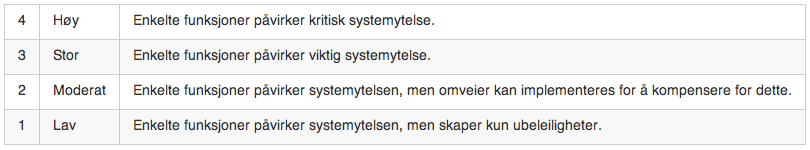
\includegraphics{Forelesning 06/img/tabell1.png}
\caption{}
\end{figure}

\paragraph{V\&V Activities}

\begin{figure}[htbp]
\centering
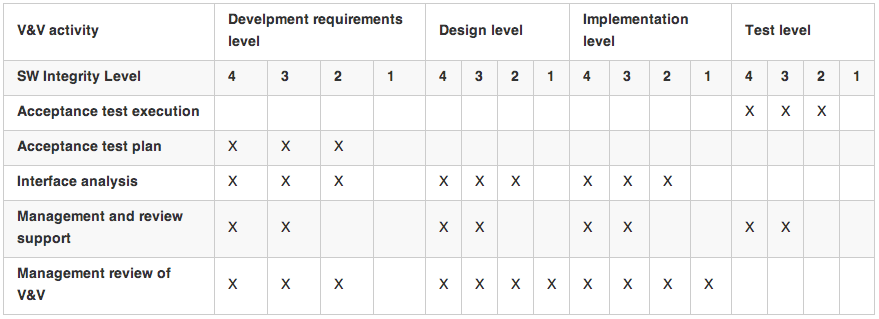
\includegraphics{Forelesning 06/img/tabell2.png}
\caption{}
\end{figure}

\subsubsection{ISO 26262 -- Automotive Software}

Her benyttes en ASIL-skala -- A, B, C, D -- som et resultat av å
kombinere tre ulike faktorer. S (severity -- hvor alvorlig en hendelse
er), E (probability -- sannsynlighet for hendelsen skal inntreffe) og C
(controllability -- hvor enkelt det er å kontrollere hendelsen dersom
den intreffer).

\paragraph{Hvordan finne ASIL-nivå}

\begin{figure}[htbp]
\centering
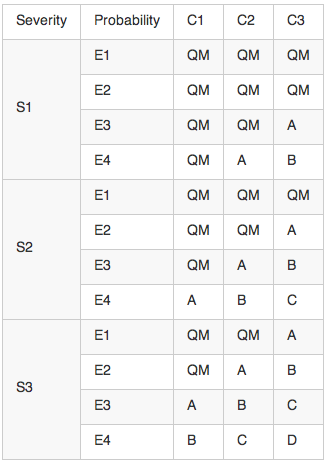
\includegraphics{Forelesning 06/img/tabell3.png}
\caption{}
\end{figure}

\subsubsection{IEC 61508 -- Safety Critical Software}

\begin{figure}[htbp]
\centering
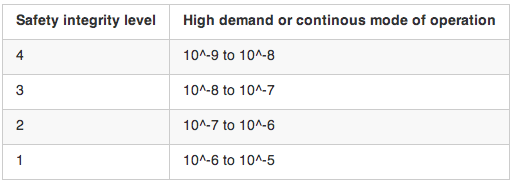
\includegraphics{Forelesning 06/img/tabell4.png}
\caption{}
\end{figure}

PFDavg = Ft / Fnp. Tabellen over gir SIL-nivå, sammen med denne verdien.

\subsection{Testobjektiver og -prioritering}

Kun i helt spesielle tilfeller kan en teste absolutt alle inndata. En må
derfor vite det overordnede målet med testingen, målsetningen med hvert
enkelt testcase, og teknikker for design av testcaser for å oppnå våre
mål på en systematisk måte.

Testobjektivene er vår kravsspesifikasjon for testing.

\subsection{Valg av testdata}

Valg av data å teste med er et av de viktigste valgene vi gjør når vi
utformer en teststrategi. Fem populære metoder er pensum i faget.

\subsubsection{Tilfeldig testing}

I denne metoden benytter en seg av to handlinger.

\begin{enumerate}[1.]
\item
  Definér alle input-parametre (integer, real, string)
\item
  Benytt en tilfeldig test/nummer-generator for å produsere inndata til
  SUT (wtf is SUT?)
\end{enumerate}
Hovedproblemet med denne metoden er mangelen på et orakel å teste
resultatene opp mot. En må med andre ord kontrollere resultatene
manuelt.

Tilfeldig testing benyttes som regel i forbindelse med
robusthetstesting, hvor en vil finne ut om et gitt system kan håndtere
(store mengder) ulike data uten å brekke.

\subsubsection{Domenepartisjoneringstesting}

Domene : Et sett input-verdier hvor programmet ufører den samme
utregningen for hvert nummer i settet. Vi ønsker å definere domene slik
at programmet utfører ulike utregninger på nærliggende domener.

Et program sies å ha en domenefeil dersom programmet velger feil domene,
input-klassifikasjonen feiler.

\subsubsection{Risikobasert testing}

Ved bruk av risikobasert testing er det to aktiviteter som en vil gå
gjennom.

\begin{enumerate}[1.]
\item
  Identifisere risiko eller kostnader ved å \emph{ikke} levere en gitt
  funksjonalitet.
\item
  Bruke denne informasjonen til å prioritere tester.
\end{enumerate}
\subsubsection{Brukerprofiltesting}

Hovedideen med brukerprofiltesting (user profile testing) er å generere
tester som gjenspeiler brukerens faktiske måte å bruke systemet. Dersom
brukerne i 80\% av tilfeller kun leser ut en verdi fra databasen, endrer
denne for så å lagre den tilbake må 80\% av testene testen denne
handlingen.

Denne testmetoden behøver dog god kunnskap til bruker og brukerdomenet.

\subsubsection{Bachs generiske risikoliste}

Se etter ting som er: * komplekse * nytt * endret * oppstrømsavhengig *
nedstrømsavhengig * kritisk * presis * populær * strategisk * tredjepart
(inkl. COTS) * distribuert * buggy * nylig svikt

\subsubsection{Test- og systemnivåer}

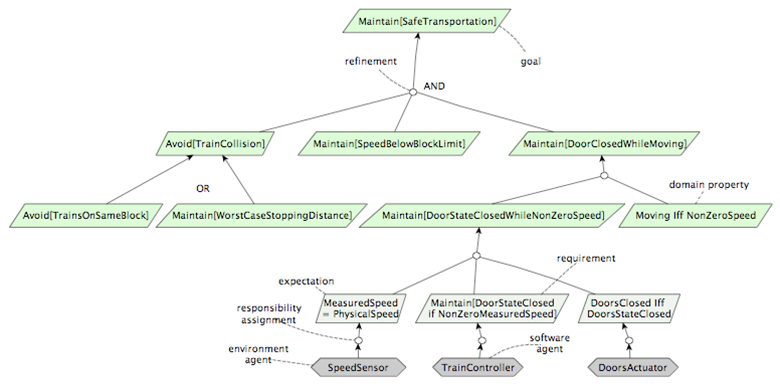
\includegraphics{Forelesning 06/img/2.png} Kan teste på ulike nivåer fra
nederst og opp : * Elektronisk nivå (DoorActuator sender riktig signal)
* State nivå (Test at døren er lukket dersom state = DoorStateClosed) *
Logisk nivå (Test at dørene er lukket så lenge man har != 0 speed,
Maintain{[}DoorStateClosedWhileNonZeroSpeed{]}) * Sikkerhetsnivå (Test
at dørene er lukket så lenge toget flytter på seg,
Maintain{[}DoorClosedWhileMoving{]})

Tester altså fra overordnede mål med multi-agenter, til requirements med
single-agent.

\section{6.3 - Grey box testing}

Testing med begrenset kunnskap av de interne delene i systemet. Med
tilgang til detaljerte designdokumenter ut over kravsspesifikasjoner.
Tester genereres basert på informasjon som tilstandsbaserte modeller
eller systemets arkitekturdiagrammer.

\subsection{Tilstandsbasert testing}

Deriveres fra forventet systemoppførsel, UML-diagrammer eller andre
typer diagrammer. De fleste systemer vil ha et enormt antall tilstander.

\subsection{Binders tilstander}

Liste over vanlige tilstandsfeil. Kan brukes som input i tilstandsbasert
testing eller statemachine/kodeinspeksjon

\begin{itemize}
\item
  Manglende eller ukorrekt tilstand
\item
  Ekstra, manglende eller korrupt tilstand
\item
  Sniksti (sneak path)
  \begin{itemize}
  \item
    Melding godtatt når den ikke skal det
  \end{itemize}
\item
  ``Ulovlig melding''-feil
\item
  Trap-door
  \begin{itemize}
  \item
    Systemet godtar udefinert melding
  \end{itemize}
\end{itemize}
Vi kan velge mellom en eller flere av disse test-utvelgelseskriteriene:
* Alle tilstander - testing passerer gjennom alle tilstandene * Alle
hendelser - testing tvinger alle hendelser til å skje minst en gang *
Alle handlinger - testing tvinger alle handlinger til å bli produsert
minst en gang

\subsubsection{Teststrategier for tilstand}

Alle round-trip-stier hvor alle sekvenser begynner og slutter i samme
tilstand. Alle enkle stier fra første til siste state, er det loops bruk
bare en iterasjon. Strategien hjelper oss til å finne alle invalide
eller manglende stier, noen ekstra tilstander og alle hendelses- og
handlingsfeil.

\subsubsection{Roundtrip path-tre}

Bygget fra et tilstandsdiagram og inkluderer alle round-trip stier(se
over). Kan brukes til å sjekke likheten mot visse behavioral models, og
kan finne snik-stier. En teststrategi basert på et round-trip path tre
vil avsløre:

\begin{itemize}
\item
  Alle kontrollfeil i tilstanden
\item
  Alle snikstier (melding godtatt når den ikke burde)
\item
  Korrupte tilstander, uforutsigbar oppførsel.
\end{itemize}
Utfordringer: Må kunne observere og registrere entitetene (aktiviteter,
triggers) for å kunne teste et system basert på disse.
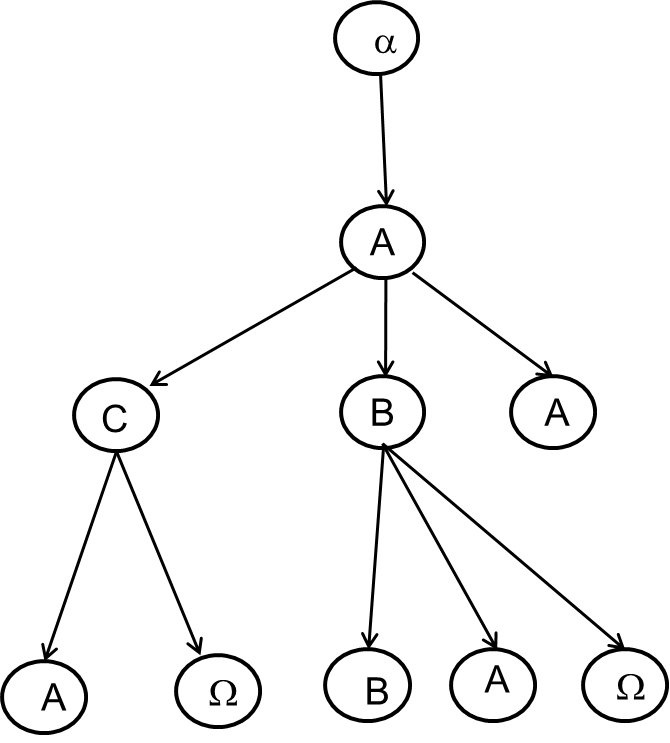
\includegraphics{Forelesning 06/img/3.png}

\paragraph{Overganger/Transitions}

Hver overgang i et tilstandsdiagram har formen
trigger-signatur{[}guard{]}/activity, hvor alle deler er valgfrie.

\begin{itemize}
\item
  Trigger signatur: Ofte en enkelt hendelse som utløser (triggers) en
  potensiell forandring i tilstand.
\item
  Guard: En boolsk condition som må være sann for at overgangen skal
  skje.
\item
  Aktivitet: En hendelse som blir gjort under overgangen.
\end{itemize}
\begin{figure}[htbp]
\centering
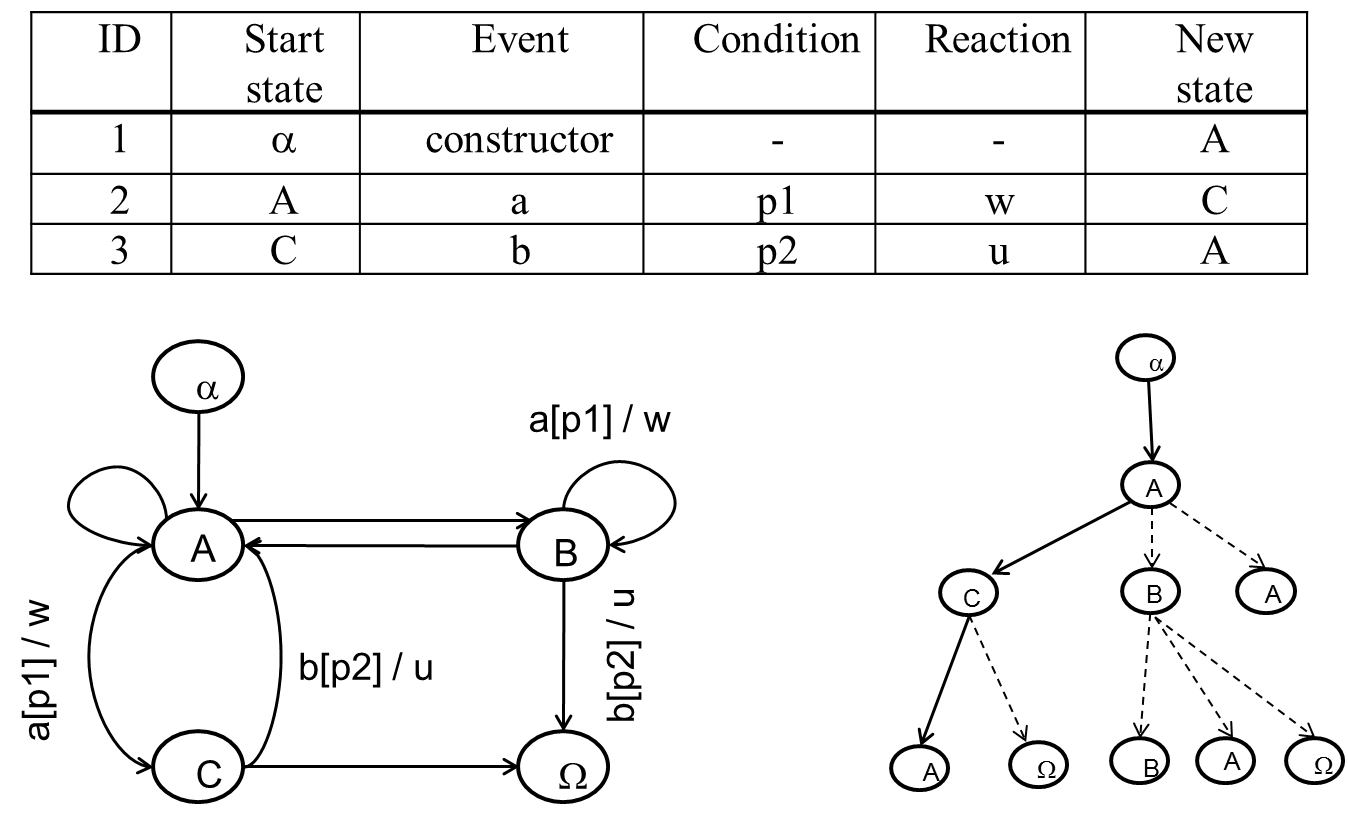
\includegraphics{Forelesning 06/img/4.png}
\caption{Testcase for alfa -\textgreater{} A -\textgreater{} C
-\textgreater{} A:}
\end{figure}

\subsubsection{Teststrategi for sniksti}

En sniksti (melding akseptert når den ikke burde) kan forekomme hvis:

\begin{itemize}
\item
  Det er en uspesifisert overgang/transition
\item
  Overgangene forekommer selv om Guard-predikatet er falskt.
\end{itemize}
\subsubsection{Sensor}

Se foiler forelesning 6 for mer eksempler

\begin{figure}[htbp]
\centering
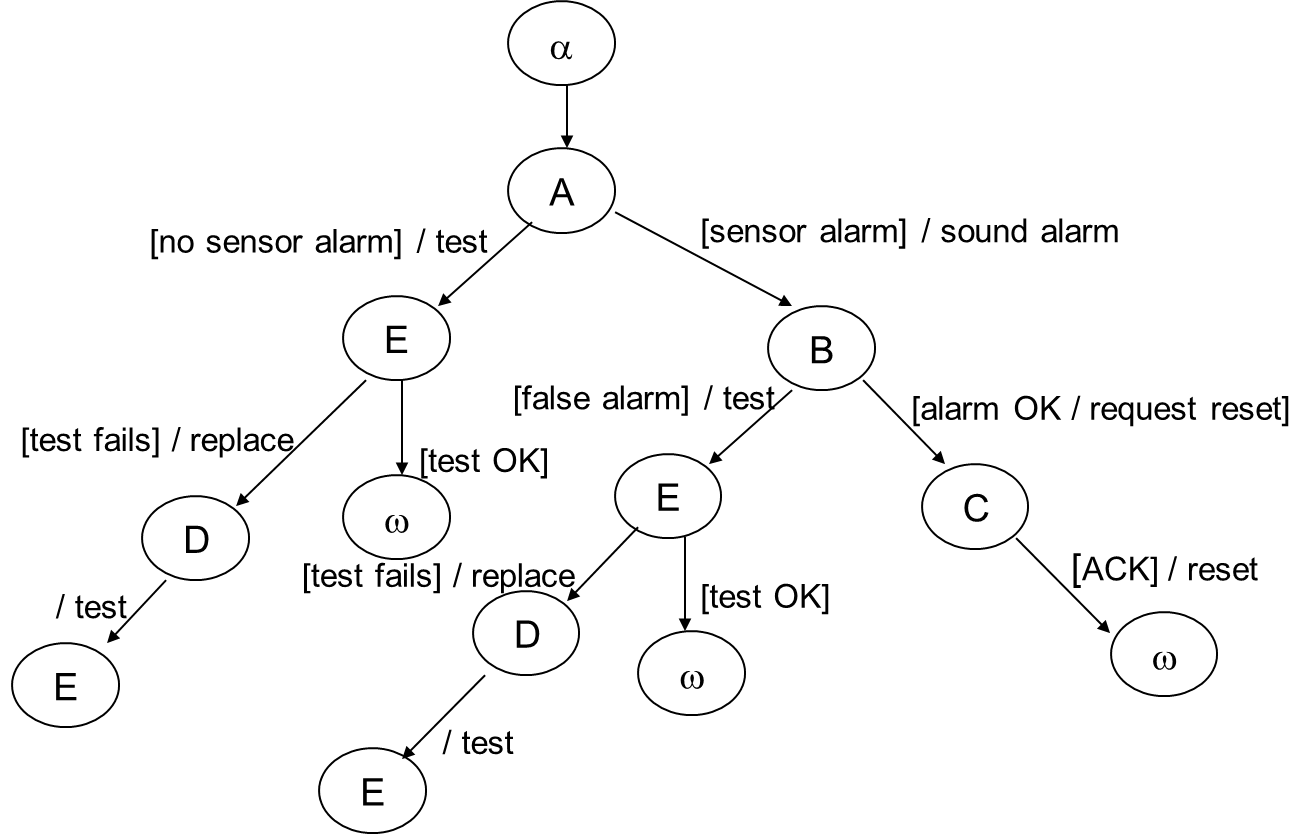
\includegraphics{Forelesning 06/img/5.png}
\caption{Sensor round-trip path tre}
\end{figure}

\section{Mutation testing}

\subsection{Type 1}

\begin{enumerate}[1.]
\item
  Skriv en kodesnutt
\item
  Skriv et sett tester
\item
  Test og korrigér til test-suite kjører uten feil
\item
  Forandre tilfeldig deler av koden (kodemutering)
\item
  Kjør test-suite igjen
\end{enumerate}
Dersom testsuiten kjører uten feil er det noe galt med test-suiten, og
den må utvides. Dersom den feiler, gå tilbake til steg 4 og skap en ny
mutant. Testeprosessen stopper når alle av X sine nye mutanter er
identifisert av den nyeste test-suiten.

\subsection{Type 2 -- fuzzing}

Har mye til felles med tilfeldig testing. Forskjellen er at vi her:
starter med input som fungerer, endre (mutér) den på en tilfeldig måte.
Viktig å tenke på at små forandringer i input kan gi store forskjeller i
output. Se foil forelesning 6.3 for eksempel på mutasjonstesting.

\subsubsection{Mutanttestingstrategier}

Antallet mutanter er stort. For å få et tålelig stort test sett må vi ha
visse strategier (referer til Papdakis og Malevris hvis man bruker de).
Mutant-teststrategier er enten av 1. eller 2. orden.

* 1. Orden: Utfør en tilfeldig seleksjon av en del av de genererte
mutantene, f.eks 10\% eller 20\% * 2. Orden: Kombinèr to mutanter til å
få en komponent å teste, her vil strategien avhenge av hvordan vi velger
mutantene.

Se foiler for eksempler:

Kommentarer til 1. orden: Måler testeffektivitet gjennom : Test
effektivitet (antall testcases / antall identifiserte feil) og
kostnadseffektivitet (antall testcases + antall ekvivalente mutanter /
antall identifiserte feil) Å velge 10\% av alle genererte mutanter er
best med tanke på kostnadseffektivitet og testeffektivitet. Såkalt
Strong mutation - bruk alle genererte mutanter- er verst.

Kommentarer til 2. orden: SU\_F2Last ( Same Unit and First combined with
Last) scorer høyest på testeffektivitet. Random mix scorer høyest på
kostnadseffektivitet. Ingen 2.ordens strategi er mer effektiv enn
Rand(10\%) strategien, hvor Fd = Antall test cases / 1.34

\section{6.2 - White box Black box Gray box}

\subsection{White box testing}

Her benytter en seg av innsikt internt i applikasjonen til å generere
tester. Denne informasjonen benyttes så for å kunne oppnå testdekning i
en eller annen for, i eksempelvis kode, stier og valgmuligheter.
Debugging vil alltid være white box.

\subsubsection{McCabes syklomatisk kompleksitet}

Flytgraf

Kompleksiteten er definert som v(G) = E - N + 2P

v(G) = syklomatisk kompleksitet E = antall kanter i grafen N = antall
noder i grafen P = antall sammenkoblede komponenter

Den sykolomatiske kompleksiteten benyttes for å definere antall
gjennomganger som er nødvendig for å kunne garantere (?) dekning for en
test.

v(G) er alltid minimum antall stier gjennom koden. Så lenge grafen er en
DAG (directed asyclic graph) vil maksimum antall stier være
2\^{}\textbar{}\{predikater\}\textbar{}

v(g) \textless{} antall stier \textless{}
2\^{}\textbar{}\{predikater\}\textbar{}

Et problem en kan stå ovenfor er løkker. En kan dog kunne se antallet
stier, selv antallet strengt tatt er ``uendelig''.

\subsubsection{Beslutningstabell}

Generell teknikk for å oppnå fullstendig testdekning, men kan i mange
tilfeller føre til overtesting.

\begin{enumerate}[1.]
\item
  Lag en tabell med alle predikater
\item
  Sett inn alle kombinasjoner av True og False for hver predikat
\item
  Konstruér en test for alle kombinasjoner
\end{enumerate}
Eksempel:

\ctable[pos = H, center, botcap]{ll}
{% notes
}
{% rows
\FL
\parbox[b]{0.11\columnwidth}{\raggedright
\emph{P1}
} & \parbox[b]{0.06\columnwidth}{\raggedright
\emph{P2}
}
\ML
\parbox[t]{0.11\columnwidth}{\raggedright
0
} & \parbox[t]{0.06\columnwidth}{\raggedright
0
}
\\\noalign{\medskip}
\parbox[t]{0.11\columnwidth}{\raggedright
0
} & \parbox[t]{0.06\columnwidth}{\raggedright
1
}
\\\noalign{\medskip}
\parbox[t]{0.11\columnwidth}{\raggedright
1
} & \parbox[t]{0.06\columnwidth}{\raggedright
0
}
\\\noalign{\medskip}
\parbox[t]{0.11\columnwidth}{\raggedright
1
} & \parbox[t]{0.06\columnwidth}{\raggedright
1
}
\LL
}

Fungerer kun i de tilfeller hvor en står ovenfor binære beslutninger, og
hvor skal teste mindre kodebolker. Legg merke at kode som er vanskelig å
nå ved at predikater som skal til for at koden skal nåes er muligens
ikke en nødvendig del av systemet.

\begin{figure}[htbp]
\centering
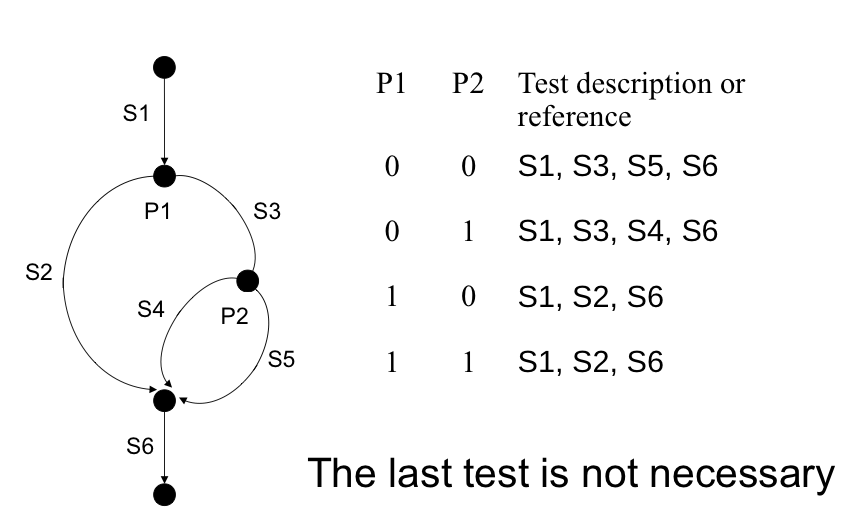
\includegraphics{Forelesning 06/img/1.png}
\caption{Beslutningstabelleksempel}
\end{figure}

\subsubsection{Løkker}

Vanlig fremgangsmåte:

\begin{itemize}
\item
  0 ganger
\item
  1 gang
\item
  5 ganger
\item
  20 ganger
\end{itemize}
På denne måten kan en teste at koden utfører løkka mange nok ganger for
å sannsynliggjøre at den fungerer som den skal.

\subsubsection{Feilmeldinger}

\begin{enumerate}[1.]
\item
  Identifisere alle feiltilstander.
\item
  Provosere frem identifiserte feiltilstander.
\item
  Kontrollere at alle feil håndteres på en tilfredsstillende måte.
  \begin{itemize}
  \item
    Dette inkluderer at eventuelle feilmeldinger inneholder den
    informasjonen brukeren behøver for å utbedre problemet.
  \end{itemize}
\end{enumerate}
\subsubsection{Videre lesning}

\href{http://en.wikipedia.org/wiki/White\_box\_testing}{Wikipedia --
White box testing}

\subsection{Black box testing}

Aka. funksjonell testing.

Utføres uten kunnskap til systemets indre. En vil mate et system med
data for så å analysere resultatet.

\begin{enumerate}[1.]
\item
  Definere initiell komponenttilstand, input og forventet output for
  testen.
\item
  Sette komponenter i definert tilstand.
\item
  Mate med definert data.
\item
  Observere output og sammenligne med forventet resultat.
\end{enumerate}
Hovedideen er at en ikke har adgang til til den koden som ligger til
grunn for programmet.

\subsubsection{Testing av sanntidssystemer}

BSP, KSP, TKSP

\subsubsection{Videre lesning}

\href{http://en.wikipedia.org/wiki/Black\_box\_testing}{Wikipedia --
Black box testing}

\subsection{Gray box testing}

Gray box er en kobinasjon av både white box- og black box-testing, og
gjøres med \emph{begrenset} kunnskap om systemets indre.

\subsubsection{Videre lesning}

\href{http://en.wikipedia.org/wiki/Gray\_box\_testing}{Wikipedia -- Gray
box testing}

\section{3 - Sporbarhet av krav}

Sporbarhet av krav er av Gotel og Finkelstein definert som:

\begin{quote}
``{[}\ldots{}{]} the ability to describe and follow the life of a
requirement, \emph{in both a forwards and backwards direction},
i.e.~from its origins, through its development and specification, to its
subsequent deployment and use, and through periods of on-going
refinement and iteration in any of the phases.''

\textbf{Gotel og Finkelstein} (1994)

\end{quote}
En legger med andre ord vekt på at alle de krav som et prosjekt har skal
være sporbare \emph{hele veien} helt fra insepsjonen via utvikling og
spesifikasjon til utplassering og bruk.

For å oppnå dette er det definert en rekke mål:

\begin{itemize}
\item
  Prosjekthåndtering
  \begin{itemize}
  \item
    Status: ``Når vil vi være ferdige?'' og ``Hva vil det koste?''
  \item
    Kvalitet: ``Hvor nære er vi å nå våre mål?''
  \end{itemize}
\item
  Håndtering av kvalitetssikring
  \begin{itemize}
  \item
    Forbedre kvalitet: ``Hva kan vi gjøre bedre?''
  \end{itemize}
\item
  Endringshåndtering
  \begin{itemize}
  \item
    Versjonering, dokumentasjon av forandringer (Hvorfor? Hva? Når?)
  \item
    Analyse av endringsinnvirkning
  \end{itemize}
\item
  Gjenbruk
  \begin{itemize}
  \item
    Varianter og produktfamilier
  \item
    Krav kan bli målrettet for gjenbruk
  \end{itemize}
\item
  Validering
  \begin{itemize}
  \item
    Finne og fjerne konflikter mellom krav
  \item
    Kravs grad av kompletthet
  \end{itemize}
\item
  Verifisering
  \begin{itemize}
  \item
    Sikre at alle krav er oppnådd
  \end{itemize}
\item
  Systeminspeksjon
  \begin{itemize}
  \item
    Identifisere alternativer og kompromisser
  \end{itemize}
\item
  Sertifisering og revisjon
  \begin{itemize}
  \item
    Bevis for at standarder følges.
  \end{itemize}
\end{itemize}
\subsection{Utfordringer}

Det foreligger en rekke utfordringer som en må ta hensyn til når det
kommer til sporing av krav. Blant disse er:

Spor må identifiseres og registreres blant et stort antall hetrogene
entiteter, instanser. Det kan være vanskelig å skape betydningsfulle
relasjoner i en slik kompleks kontekst.

Spor er videre i konstant forandring og bevelgelse, ettersom de vil
kunne forandres ved forandringer i krav eller utviklingsartefakter.

Stor variasjon i verktøy, basert på matriser, hyperlenker, tagging,
identifiers. Fortsatt må det meste av arbeidet utføres manuelt.

Sporinformasjonen er aldri komplett. Dette grunnet komplekse systemer av
sporingservervelse og -vedlikehold.

Grunnet mangel på kvalitetsattributter er tillit en stor utfordringer.
Det nytter eksempelvis ikke at en vet at 70\% av alle sporingskoblinger
er nøyaktige om en ikke samtidig vet hvilke koblinger som utgjør disse
70\%.

Prosjektet har gjerne en rekke ulike interessenter. Disse har ulikt syn
på prosjektet avhengig av sin rolle. Disse vil følgelig ha ulike syn på
sporbarheten av krav.

Håndtering av kvalitetssikring handler om å maksimere et produkts
\emph{kvalitet}. Denne kvaliteten skal være dokumentert i
kravsspesifikasjonen, og spørsmål som derfor spørres i denne
sammenhengen er \emph{``Hvor nære er vi kravsspesifikasjonen vår?''} og
\emph{``Hva kan vi gjøre bedre?''}.

Endringshåndtering handler om å spore effektene av hver enkelt endring.
Dette gjøres ofte via firewall, etc.

Gjenbruk vil peke på de aspekter av en gjenbrukt komponent som behøves
adapteres til de nye systemkravene. Til og med kravene i seg selv kan
være ting som kan gjenbrukes.

Validering vil bruke sporbarheten til å peke på kravenes kvalitetet når
det kommer til kompletthet, tvetydighet, forward referencing, opasitet
(tetthet). Vil også sikre at hvert av kravene dekkes av minst én del av
produktet

Verifikasjon vil sjekke at de begrensninger en har overholdes.

I tillegg kommer det utfordringer relatert til sertifisering/audit, samt
testing og vedlikehold.

\subsection{Metamodeller}

Modell : En abstraksjon av virkeligheten.

Metamodell : Modeller av modeller, en videre abstraksjon av
virkeligheten som belyser egenskaper ved modellen.

Metamodeller for sporbarhet av krav benyttes ofte som basis for
sporbarhetsmetodologier og -rammeverk. Dette for å kunne fastslå og
definere hvilke typer artefakter som skal spores, samt definere hvilke
typer relasjoner som kan etableres mellom disse artefaktene.

{[}STAKEHOLDER{]} --Manages--\textgreater{} {[}SOURCE{]}
--Documents--\textgreater{} {[}OBJECT{]}

{[}STAKEHOLDER{]} --Has role in --\textgreater{} {[}OBJECT{]}

{[}OBJECT{]} --Traces to--\textgreater{} {[}OBJECT{]}

{[}STAKEHOLDER{]} --Has role in --\textgreater{} --Traces
to--\textgreater{} {[}OBJECT{]}

Der skilles ofte mellom high-end- og low-end-sporbarhet.

\begin{figure}[htbp]
\centering
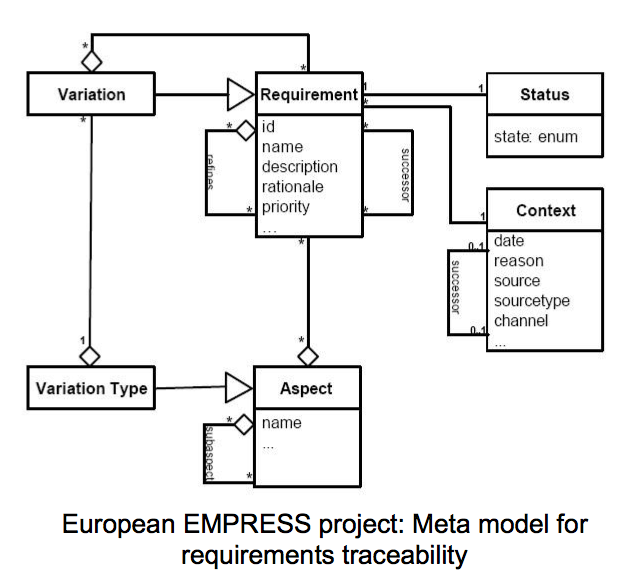
\includegraphics{Forelesning 03/img/3.png}
\caption{European EMPRESS project: Meta model for requirements
traceability}
\end{figure}

\begin{figure}[htbp]
\centering

\includegraphics{Forelesning 03/img/4.png}
\caption{PRECISE Meta-model (SINTEF)}
\end{figure}

\subsection{Tilnærminger til sporbarhet}

Det er en kritisk oppgave å kunne etablere koblinger, både mellom ulike
krav, og mellom krav og andre artefakter. Manuell kobling og vedlikehold
av slike koblinger er både dyrt og utsatt for feil. En ønsker derfor å
kunne helt eller delvis automatisere denne oppgaven.

\subsubsection{Manuell sporingskobling}

Manuell sporingskobling er den enkleste formen for sporbarhet. Her
benytter en seg av \emph{sporbarhetsmatriser}, enten ved bruk av
hypertekst eller regnearkprogram som for eksempel Microsoft Excel for å
skape kryssreferanseskjema. Der er i hovedsak to problemer med denne
tilnærmingen: over tid vil det å vedlikeholde et stort antall koblinger
bli vanskelig; og da koblingene er statiske (mangel på attributter) vil
mangel på automasjon av oppgaver være begrenset.

\ctable[pos = H, center, botcap]{lllllllll}
{% notes
}
{% rows
\FL
\parbox[b]{0.09\columnwidth}{\raggedright
Unik ID Krav
} & \parbox[b]{0.09\columnwidth}{\raggedright
Kilde til krav
} & \parbox[b]{0.20\columnwidth}{\raggedright
SW-krav-spek./ Funk. krav. dok.
} & \parbox[b]{0.09\columnwidth}{\raggedright
Design-spek.
} & \parbox[b]{0.09\columnwidth}{\raggedright
Program-modul
} & \parbox[b]{0.09\columnwidth}{\raggedright
Test-case(r)
} & \parbox[b]{0.17\columnwidth}{\raggedright
Vellykket test-verifikasjon
} & \parbox[b]{0.13\columnwidth}{\raggedright
Modifikasjon av krav
} & \parbox[b]{0.07\columnwidth}{\raggedright
Bemerkninger
}
\ML
\parbox[t]{0.09\columnwidth}{\raggedright
\ldots{}
} & \parbox[t]{0.09\columnwidth}{\raggedright
\ldots{}
} & \parbox[t]{0.20\columnwidth}{\raggedright
\ldots{}
} & \parbox[t]{0.09\columnwidth}{\raggedright
\ldots{}
} & \parbox[t]{0.09\columnwidth}{\raggedright
\ldots{}
} & \parbox[t]{0.09\columnwidth}{\raggedright
\ldots{}
} & \parbox[t]{0.17\columnwidth}{\raggedright
\ldots{}
} & \parbox[t]{0.13\columnwidth}{\raggedright
\ldots{}
} & \parbox[t]{0.07\columnwidth}{\raggedright
\ldots{}
}
\LL
}

\subsubsection{Scenario-drevet sporbarhet}

Scenario-drevet sporbarhet er en \emph{testbasert} tilnærming som
benyttes for å avdekke relasjoner mellom krav, design og kodeartefakter.
\href{http://www.alexander-egyed.com/publications/A\_Scenario-Driven\_Approach\_to\_Traceability.pdf}{Alexander
Egyed} er anerkjent som forfatteren av denne tilnærmingen.

Trikset benyttet er å observere kjøretids-oppførselen til
testscenarioer. Eksempler på verktøy som benytter seg av denne
tilnærmingen er \href{http://www.jfind.com/listings/1711.shtml}{IBM
Rational PureCoverage}. Kjøretidsoppførselen til applikasjonen
oversettes til en grafstruktur som benyttes til å indikere fellestrekk
mellom entiteter assosiert med hendelsen.

Metoden benytter seg av det den kaller et \emph{footprint} for å oppnå
sporbarhet. Dette fotsporet inneholder informasjon om det settet klasser
som ble eksekvert når et spesifisert scenario testes, og antallet
metoder som ble eksekvert i hver av disse klassene.

Eksempel:

\ctable[pos = H, center, botcap]{llll}
{% notes
}
{% rows
\FL
\parbox[b]{0.09\columnwidth}{\raggedright
} & \parbox[b]{0.43\columnwidth}{\raggedright
\emph{Test-scenario}
} & \parbox[b]{0.17\columnwidth}{\raggedright
\emph{Artefakt}
} & \parbox[b]{0.30\columnwidth}{\raggedright
\emph{Observerte Java-klasser}
}
\ML
\parbox[t]{0.09\columnwidth}{\raggedright
1
} & \parbox[t]{0.43\columnwidth}{\raggedright
Se liste over filmer
} & \parbox[t]{0.17\columnwidth}{\raggedright
{[}s3{]}
} & \parbox[t]{0.30\columnwidth}{\raggedright
{[}C, J, R, U{]}
}
\\\noalign{\medskip}
\parbox[t]{0.09\columnwidth}{\raggedright
2
} & \parbox[t]{0.43\columnwidth}{\raggedright
Se kontekstuell informasjon om film
} & \parbox[t]{0.17\columnwidth}{\raggedright
{[}s4, s6{]} {[}r2{]}
} & \parbox[t]{0.30\columnwidth}{\raggedright
{[}C, E, J, N, R{]}
}
\\\noalign{\medskip}
\parbox[t]{0.09\columnwidth}{\raggedright
3
} & \parbox[t]{0.43\columnwidth}{\raggedright
Velg/spill av film
} & \parbox[t]{0.17\columnwidth}{\raggedright
{[}s8, s9{]} {[}r6{]}
} & \parbox[t]{0.30\columnwidth}{\raggedright
{[}A, C, D, F, G, I, J, K, N, O, T, R, U{]}
}
\\\noalign{\medskip}
\parbox[t]{0.09\columnwidth}{\raggedright
4
} & \parbox[t]{0.43\columnwidth}{\raggedright
Trykk stopp-knapp
} & \parbox[t]{0.17\columnwidth}{\raggedright
{[}s9, s11{]} {[}r8{]}
} & \parbox[t]{0.30\columnwidth}{\raggedright
{[}A, C, D, E, F, G, I, K, O, T, U{]}
}
\\\noalign{\medskip}
\parbox[t]{0.09\columnwidth}{\raggedright
5
} & \parbox[t]{0.43\columnwidth}{\raggedright
Trykk spill-knapp
} & \parbox[t]{0.17\columnwidth}{\raggedright
{[}s9, s11{]} {[}r9{]}
} & \parbox[t]{0.30\columnwidth}{\raggedright
{[}A, C, D, F, G, I, K, N, O, T, R, U{]}
}
\\\noalign{\medskip}
\parbox[t]{0.09\columnwidth}{\raggedright
6
} & \parbox[t]{0.43\columnwidth}{\raggedright
Bytt server
} & \parbox[t]{0.17\columnwidth}{\raggedright
{[}s5, s7{]}
} & \parbox[t]{0.30\columnwidth}{\raggedright
{[}C, R, J, S{]}
}
\\\noalign{\medskip}
\parbox[t]{0.09\columnwidth}{\raggedright
7
} & \parbox[t]{0.43\columnwidth}{\raggedright
\ldots{}
} & \parbox[t]{0.17\columnwidth}{\raggedright
\ldots{}
} & \parbox[t]{0.30\columnwidth}{\raggedright
\ldots{}
}
\LL
}

Det er imidlertid noen problemer tilknyttet til denne tilnærmingen. Det
en kan komme over er at der finnes scenarioer som ikke dekker noen krav,
og der kan finnes scenarioer som hører til flere krav. Slike hendelser
må markeres i en separat tabell. En benytter seg her av symbolene ``F''
(fixed) og ``P'' (probable) for å markere et tilfelle, avhengig av hvor
sikre vi er på at en gitt klasse tilhører et gitt scenario.

\begin{figure}[htbp]
\centering

\includegraphics{Forelesning 03/img/5.png}
\caption{Eksempel}
\end{figure}

\subsubsection{Utviklingsfotspor}

Utviklingsfotspor (development footprint) er en løsning som gjør det
mulig å skape sporbarhetsinformasjon, utviklet av (Inah
Omoronyia){[}http://www.informatik.uni-trier.de/\ensuremath{\sim}ley/db/indices/a-tree/o/Omoronyia:Inah.html{]}
et al. Denne metoden krever at hver utvikler alltid identifiserer det
krav/use-case som han/hun jobber med på et gitt tidspunkt. En utvikler
kan kun jobbe med et enkelt use-case om gangen.

Resultatet av denne metoden vil være lik den som ved bruk av
scenario-test-footpring-tabellen. Denne tabellen vil vise hvilke
dokumenter, classer og lignende som har blitt aksessert gjennom arbeid
med en gitt use-case.

Hovedproblemet med denne tilnærmingen er at det forekommer ``falske''
adganger. Dette kan skje eksempelvis ved at en utvikler ser på en del av
koden som ikke tilhører det use-case som det på et gitt tidspunkt jobbes
med. For å motvirke dette kan en supplere informasjonen som genereres
med mer informasjon om en aksess' natur, tidspunkt og person som utførte
aksesseringen.

Typer aksesseringstyper gitt i denne metoden er:

\begin{itemize}
\item
  C - Create
\item
  U - Update
\item
  V - View
\end{itemize}
\begin{figure}[htbp]
\centering
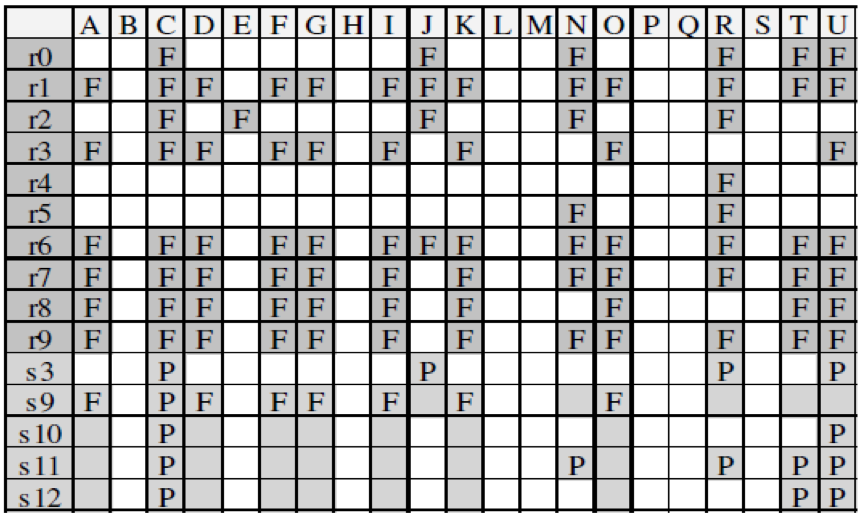
\includegraphics{Forelesning 03/img/6.png}
\caption{Eksempel på bruk av developer footprint}
\end{figure}

\subsubsection{Ulemper ved bruk av scenario-drevet sporbarhet}

Selv om scenario-drevet sporbarhet ofte er semi-automatiserte trenger de
allikevel mye tid av systemingeniører som iterativt må identifisere et
subsett testscenarioer og hvordan disse relaterer til kravsartefakter.
Videre er det ikke alltid at krav som per metodene gitt over ikke er
relaterte, ikke er relaterte i en annen form (som for eksempel deling av
data, implementasjons-pattern).

Jeg ser for meg det er her Singleton-patternet kan være problematisk
(TK).

\subsection{Sporing via tagging}

Denne metoden er enkel både å forstå og å implementere. Ulempen er dog
at den er sterkt avhengig av menneskelig innblanding. Prinsippet med
tagging er at hver enkelt krav gis en \emph{tagg}, enten manuelt eller
av et verktøy. Hvert enkelt dokument, kodesnutt, etc. gis også hver sin
tagg.

Ulike fremgangsmåter kan benyttes -- tagger kan være enten enkeltnivå
eller flernivå. Ved bruk av enkeltnivå (eks. R4) får en en enkel
sporingsmatrise. Ved bruk av flernivå-tagger (eks. hvor R4.1 og R4.2 er
sub-nivå av R4) vil en enkelt kunne gruppere logiske grupperinger av
krav, og en kan dermed få mer detaljert sporingsinformasjon.

Sporbarhetens kvalitet vil bero på at vi alltid husker å (korrekt) tagge
alle relevante dokumenter og artefakter. Der finnes verktøy som kan
kontrollere at alle dokumenter i databasen er tagget, men korrektheten
av disse taggene er derimot ikke gitt.

\subsection{Konklusjon}

Det å kunne spore krav er et svært viktig aspekt ved kravshåndtering.

Prosjektets ulike interessenter har ulike behov for
sporbarhetsinformasjon.

Sporbarhet kan være komplekst for ikke-trivielle prosjekter.

Sporbarhet-meta-modeller gir en insikt på typen sporbarhetsinformasjon
som kreves for et prosjekt.

Der eksisterer flere automatiserte tilnærminger for sporing av krav. Da
de ulike automatiserte tilnærmingene har ulike styrker og svakheter vil
den beste måten å benytte seg av disse ligge i kombinere disse riktig og
dra nytte av synergieffekter dette gir.

\subsection{Nyttige lenker}

\begin{itemize}
\item
  \href{http://en.wikipedia.org/wiki/Requirements\_traceability}{Requirements
  traceability (wikipedia.org)}
\end{itemize}
\section{Kravsspesifikasjon og testing}

Testability : The capability of the software product to enable modified
software to be validated. (ISO 9126)

Testbarhet tar for seg to hovedområder: hvor enkelt det er å teste en
gitt implementasjon; og hvor \emph{test-vennlig} et gitt krav er. Disse
to problemene er ikke uavhengige av hverandre og må alltid sees på
sammen.

\subsection{Testabilitet}

For å kunne være testbart må et gitt krav være definert på en konkret
måte. \emph{``When the ACC system is turned on, the \textbf{Active}
light on the dashboard shall be turned on.''} er et eksempel på et krav
som er tilstrekkelig definert. Dette i motsetning til \emph{``The system
shall be easy to use''} som må endres for å gjøres testbart. En metode
som brukes for å få et slikt krav mer definert og testbart er å bruke
din indre 4-åring og spørre \emph{``Hva mener du med det''} repetetivt
til du får et krav som er mer kvantitativt testbart (\emph{``Systemet
skal kunne brukes effektiv etter tre dagers bruk''}).

Der er i hovedsak tre måter å kontrollere at en har oppnådd ens mål:
\emph{\textbf{T}est-eksekvering} (inkluderer black, white og grey
box-testing); gjennom å \emph{gjøre \textbf{E}ksperimenter} og
\emph{kode\textbf{I}nspeksjon}.

\begin{figure}[htbp]
\centering
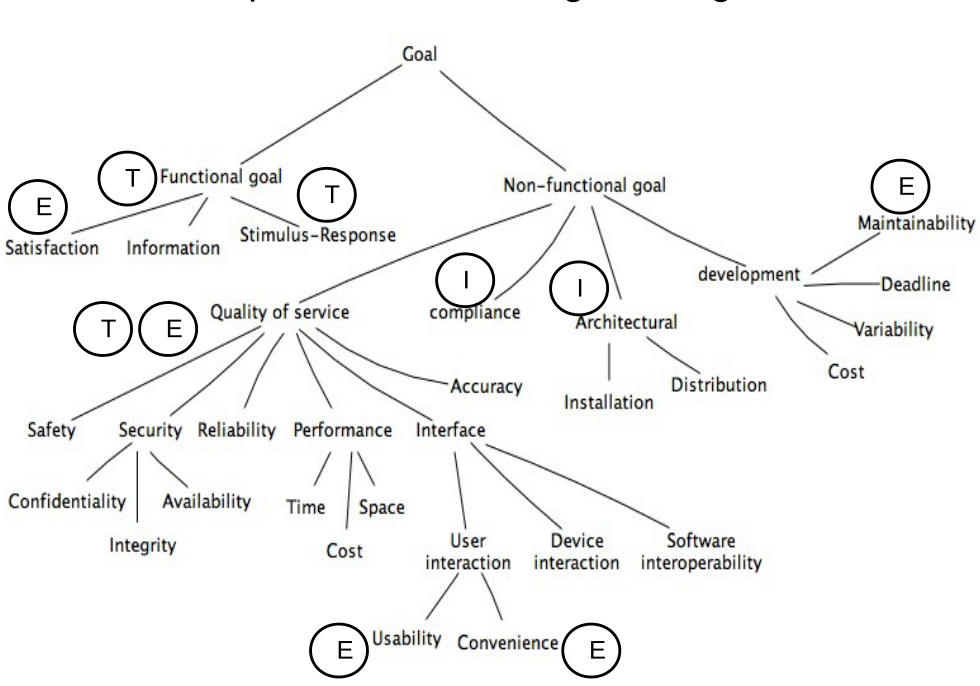
\includegraphics{Forelesning 03/img/1.png}
\caption{Konkrete krav fra høynivå-mål}
\end{figure}

\subsection{Utfordringer}

Problemer relatert til:

\begin{itemize}
\item
  Volumet til testene som skal utføres
  \begin{itemize}
  \item
    responstid, lagringskapasitet
  \end{itemize}
\item
  Typen hendelse som skal testes
  \begin{itemize}
  \item
    feilhåndtering, sikkerhetsmekanismer
  \end{itemize}
\item
  Systemets tilstand før det skal testes
  \begin{itemize}
  \item
    uvanlig feiltilstand, en gitt transaksjonshistorikk
  \end{itemize}
\end{itemize}
\subsubsection{Design by Objective}

\begin{itemize}
\item
  Tom Gilb
\end{itemize}
Der er imidlertid to problemer med denne metoden. For det første kan
testene som metoden resulterer i være svært ekstensive, og dermed dyre.
For det andre krever metoden tilgang til systemets sluttbrukere.

\begin{enumerate}[1.]
\item
  What do you mean by ? This will give us either (a) a testable
  requirement or (b) a set of testable and non-testable
  sub-requirements.
\item
  In case (a) we are finished. In case (b) we will repeat question 1 for
  each non-testable sub-requirements.
\end{enumerate}
Der kan oppstå problemer knyttet til definering av systemets tilstander.
Dersom et krav sier at et flys \emph{reverse thrust} skal kunne
reverseres \emph{kun når flyet har landet}, er det et
definisjonsspørsmål for hva som defineres som \emph{landet}. Dette blant
annet på grunn av de ulike sensorer som skal rapportere dette.

I flyeksemplet kan et svar på dette være er at et fly har landet når en
gitt vekt hviler på landingshjulene. Dette kan imidlertid være
problematisk når flyet skal lande i motvind, og dermed genererer ekstra
oppdrift, slik at flyet ikke vil kunne \emph{lande} etter de
definisjonen.

Først og fremst må kunden vite nøyaktig \emph{hva} han vil og
\emph{hvorfor} han vil ha det. Det er ofte mye enklere å teste om
kundens oppnår sine mål med applikasjonen enn det er å teste at et
system oppfyller et gitt krav. \emph{Hvorfor} er dog sjeldent en del av
en kravsspesifikasjon.

\subsubsection{Krav til testbarhet}

En rekke andre krav ligger til grunn for en god kravsspesifikasjon. Et
krav må være:

\paragraph{Korrekt}

Uten feil.

\paragraph{Komplett}

Må dekke alle situasjoner, ``dersom X så\ldots{}'' og ``dersom Y
så\ldots{}''. \emph{Må også dette de tilfeller hvor X og Y ikke
inntreffer.} Alt som ikke defineres er per definisjon utenfor
kravsspesifikasjonen og skal ikke være tilstede.

\paragraph{Konsistent}

Et krav kan ikke være i konflikt med andre krav. Dette kan være en
utfordring da vi da trenger en komplett oversikt over alle krav. Vi kan
dog i de fleste tilfeller klare oss med å kontrollere alle krav som er
relatert til samme hendelse, funksjon eller parameter.

\paragraph{Tydelig}

Konsepter av viktighet her er diagramnotasjon, beskrivelsesspråk og
detaljnivå. Dette må tilpasses til den som er ment å lese dokumentene,
det være kunde, utviklere eller testere.

\paragraph{Relevant}

Her vil en søke svaret på to spørsmål: ``\emph{Behøver vi virkelig dette
kravet?}''; og ``\emph{Er kravet så strikt som det burde være?}''. For
den som skal teste vil sistnevnte spørsmål være av viktighet, da et krav
som er for strikt vil svare til mer arbeid for utvikleren, og et for
slakt krav vil svare til mer arbeid for testeren.

\paragraph{Oppnåelig}

En må spørre seg selv om et krav i det hele tatt er mulig å oppfylle.
Testerene kan være med i denne diskusjonen ved å hele tiden spørre om
hvordan et gitt krav er ment å testes. Dette vil kunne tvinge alle
involverte parter til å gjøre hvert krav bedre definert.

Dersom et krav er vanskelig å implementere vil det ofte og være
vanskelig å teste.

\paragraph{Sporbart}

Hvert enkelt krav må kunne relateres til et eller flere: *
programvarekomponenter * prosessteg

\subsubsection{Noen tips til utforming av krav}

Unngå modifiserende fraser som ``etter nødvendighet'' og ``skal minimum
gjøre X''. Dette kan tolkes svært ulikt av ulike oppdragstakere, og en
kan i beste fall kun være sikret et absolutt minimum. Vær klar i
formuleringen!

Unngå bruk av vage ord som ``flagg'', ``håndtér'', ``spor''.
Informasjonssystemer \emph{mottar}, \emph{lagrer}, \emph{kalkulerer},
\emph{rapporterer} og \emph{sender} data, og vi bør helst bruke disse
ordene for beskrive hva systemet skal gjøre.

Unngå bruk av udefinerte pronomen, som for eksempel ``\emph{det skal
vises på skjermen}''. Dette krever at \emph{det} defineres like før, og
justeringer og endringer i rekkefølgen på krav kan ødelegge kravet
fullstendig. En må og unngå bruk av ``alle'', ``få'', ``andre'', etc. da
disse er plassholdere for ikke-navngitte individer og er åpne for
tolkning. Bruk \emph{navnet skal vises på skjermen} hver gang.

Unngå bruk av passiv stemme. Ikke definér at ``\emph{Z skal
kalkuleres}'', men heller ``\emph{Systemet skal kalkulere Z}''.

Angående negative krav, vil i prinsippet \emph{alt} som ikke er definert
i kravsspesifikasjonen være noe som systemet \emph{ikke} skal gjøre.
Bytt derfor ut alle tilfeller hvor spesifikasjonen sier noe om hva
systemet ikke skal gjøre til aktive definisjoner på hva systemet
\emph{skal} gjøre -- fra ``\emph{systemet skal ikke godta X}'' til
``\emph{systemet skal forhindre Y}''.

Alle antakelser og sammenligninger må klart definerte. Det å anta status
quo og peke på at systemet skal føre til ``15\% høyere throughput''
eller ``systemet skal adressere brukernes fremtidige behov'' vil alltid
peke mot framtiden og aldri kunne oppnåes.

\subsubsection{Implementasjonen}

\paragraph{Autonomitet}

Hvor mange andre systemer må være på plass for å teste et gitt krav? Der
er en overhengende fare for at en må planlegge og implementere mer eller
mindre komplekse ``stubber'' som tar for seg manglende systemer.

\paragraph{Observerbarhet}

Da ikke alle tester produserer utdata vi to spørsmål være viktig å
besvare i slike tilfeller: Hvor enkelt er det å observere en
testutførings progresjon?; og Hvor enkelt er det å observere et
testresultat?

\paragraph{Gjentesteffektivitet (re-test efficiency)}

Hvor enkelt er det å utføre
``test-kontrollér-forandre-gjentest''-sykelen? Dette inkluderer både
testens observerbarhet og sporbarhet.

\paragraph{Test-gjenstartbarhet (test restartability)}

Hvor enkelt er det å stoppe testen midlertidig? Hvor enkelt er det å
studere nåværende tilstand og utdata? Hvor enkelt er det å starte testen
fra det punktet den ble stoppet? Hvor enkelt er det å starte testen fra
start?

\subsection{Oppsummering}

For å sikre at et krav er testbart er det viktig at testere involveres
helt fra starten av prosjekter, og at tester er en integrert del av
kravet.

Legg merke til at selv om et krav er testbart betyr ikke dette at et
krav er \emph{enkelt} å teste.

\section{2.1 - Intro}

\subsection{Traceability}

From test to requirement : Why do we need this test?

From requirement to test : Where is this requirement tested?

Når en skal endre/justere et krav kan en også finne relevante tester.

\subsection{Challenges}

Funksjonelle (Hva et system må gjøre) vs.~ikke-funksjonelle(hvor bra
systemet utfører funksjonene) ``Defined operational capabilities
-\textgreater{} Satisfy business needs''

\ctable[pos = H, center, botcap]{ll}
{% notes
}
{% rows
\FL
\parbox[b]{0.39\columnwidth}{\raggedright
\emph{Factor}
} & \parbox[b]{0.35\columnwidth}{\raggedright
\emph{Percentage of responses}
}
\ML
\parbox[t]{0.39\columnwidth}{\raggedright
Incomplete Requirements
} & \parbox[t]{0.35\columnwidth}{\raggedright
13,1\%
}
\\\noalign{\medskip}
\parbox[t]{0.39\columnwidth}{\raggedright
Lack of User Involvement
} & \parbox[t]{0.35\columnwidth}{\raggedright
12,4\%
}
\\\noalign{\medskip}
\parbox[t]{0.39\columnwidth}{\raggedright
Lack of Resources
} & \parbox[t]{0.35\columnwidth}{\raggedright
10,6\%
}
\\\noalign{\medskip}
\parbox[t]{0.39\columnwidth}{\raggedright
Unrealistic Expectations
} & \parbox[t]{0.35\columnwidth}{\raggedright
9,9\%
}
\\\noalign{\medskip}
\parbox[t]{0.39\columnwidth}{\raggedright
Lack of Executive Support
} & \parbox[t]{0.35\columnwidth}{\raggedright
9,3\%
}
\\\noalign{\medskip}
\parbox[t]{0.39\columnwidth}{\raggedright
Challenging Requirements
} & \parbox[t]{0.35\columnwidth}{\raggedright
8,7\%
}
\\\noalign{\medskip}
\parbox[t]{0.39\columnwidth}{\raggedright
Lack of Planning
} & \parbox[t]{0.35\columnwidth}{\raggedright
8,1\%
}
\\\noalign{\medskip}
\parbox[t]{0.39\columnwidth}{\raggedright
Didn't need it any longer
} & \parbox[t]{0.35\columnwidth}{\raggedright
7,5\%
}
\\\noalign{\medskip}
\parbox[t]{0.39\columnwidth}{\raggedright
Lack of IT Management
} & \parbox[t]{0.35\columnwidth}{\raggedright
7,3\%
}
\\\noalign{\medskip}
\parbox[t]{0.39\columnwidth}{\raggedright
Technology Illiteracy
} & \parbox[t]{0.35\columnwidth}{\raggedright
9,9\%
}
\LL
}

\subsection{Krav utvikling}

Requirements Elicitation (Hvordan man kommer frem til krav) : Prosessen
der man finner kravene til et system gjennom kommunikasjon med kundene,
systembrukerne og andre stakeholders(interessenter). \emph{Teknikker}:
Metodisk ekstraksjon av konkrete krav fra høynivå mål.
kvalitetsmålprioritet til krav. (Quality Metrics)

\emph{Eksempler på ikke-tilfredstillende krav:} Ariane 5: Et dyrt
rakettoppskytingsystem. Her antok man visse parametre fra forløperen
Ariane 4, som viste seg å ikke stemme. Dette førte til selvdestruksjon
og 500mill euro i dass. Airbus: Krav: Revers kan bare brukes når flyet
har landet. Oversettelse: Revers kan bare bruke mens hjulene roterer.
Implementasjon: Revers kan bare brukes mens hjulene roterer fort nok.
Situasjon: Regnstorm og vannplaning, noe som resulterer i et krasj fordi
reversen ikke kan benyttes (siden hjulene ikke roterer). Viktig å være
nøye i modelleringen. Fun fact: Dette er et problem som fortsatt ikke er
løst. Tenk på det neste gang du er ute og flyr!

Formålet med smidig utvikling : utsette så mange avgjørelser så mye som
mulig for å øke graden av frihet til ens forståelse er god nok. Øke
forståelse ved å ta med folk som kan noe om lignende problemer.

Skille mellom kunde og faktisk bruker. Kjøper for å løse et
(\emph{konkret}?) problem.

\subsection{Two types of requirements statements}

Deskriptive statements : Observasjon av den virkelige verden, uavhengig
av systemets oppførsel. Eks: Er togdørene åpne er de ikke lukket.

Preskriptive statements : Beskriver ønskelige egenskaper om systemet,
som kan stemme avhengig av hvordan systemet oppfører seg. : Slik
tilstanden oppfattes av systemet. : Enforced \textbf{solely} by the
software-to-be. Formulert av fenomen som deles mellom programvare og
miljø. : Programvare forstår dette via sensorer, handler med aktuatorer.
Eks : Togdører skal alltid være lukket mens toget beveger seg.

\subsubsection{Formulering av systemkrav}

Eksempel: Alle togdører skal være lukket mens toget beveger seg. I
tillegg til denne preskriptive uttalelsen trenger vi hjelp fra andre
komponenter: Togkontrolleren som er ansvarlig for trygg dørkontroll.
Passasjerene må ikke åpne dører på en utrygg måte. At dørene fungerer
skikkelig (agentene).

\subsection{Domeneegenskaper}

En domeneegenskap: Er en deskriptiv uttalelse om et problem. Uttalelsen
burde holde uansett hvordan systemet oppfører seg, og er ofte i relasjon
med fysiske lover. Eks: Et tog flytter seg kun hvis farten er !0 (ikke
0).

\subsection{Målorientering}

Et mål er et mål systemet skal oppnå. Kan være alt fra høynivå
strategier til lavnivå tekniske bekymringer. Systemet består av både
programvaren og miljøet, interaksjon mellom agenter (enheter, mennesker,
programvare).

\begin{itemize}
\item
  Mål kan være på forskjellig nivå:
  \begin{itemize}
  \item
    Høynivå: Et mål krever koordinering mellom mange agenter. Eks:
    Systemets transportkapasitet skal økes med 50\%
  \item
    Krav: Et mål som en enkelt agent har ansvaret for i \emph{systemet}.
  \item
    Forventning: Et mål som en enkelt agent har ansvaret for i
    \emph{miljøet til systemet}.
  \end{itemize}
\end{itemize}
\begin{figure}[htbp]
\centering
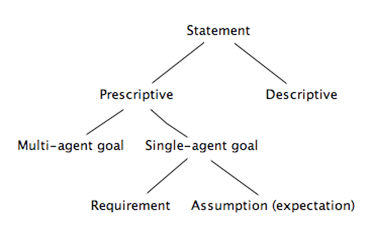
\includegraphics{Forelesning 02/img/2.png}
\caption{Goal statement typologi}
\end{figure}

\subsubsection{Typer mål}

\begin{itemize}
\item
  Soft goals
  \begin{itemize}
  \item
    Eks: Passengers should be better informed about flights.
  \item
    Improve
  \item
    Maximise/minimise
  \item
    Increase/reduce
  \end{itemize}
\item
  Behavioural goal
  \begin{itemize}
  \item
    System behaviour
  \item
    Agent behaviour
  \item
    Achieve/Cease
  \item
    Maintain/Avoid
  \end{itemize}
\end{itemize}
\subsection{Målkategorisering}

\begin{figure}[htbp]
\centering
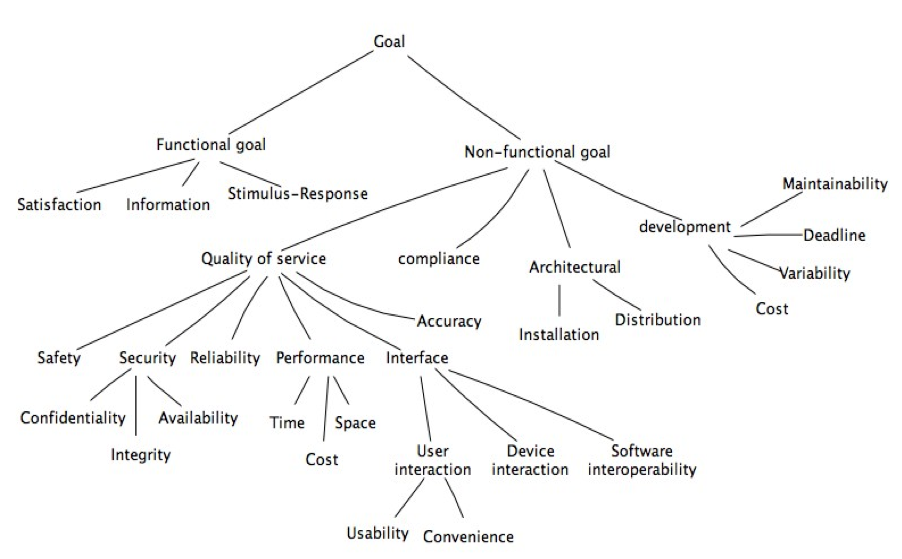
\includegraphics{Forelesning 02/img/goal-categorisation.png}
\caption{Goal categorisation}
\end{figure}

\begin{itemize}
\item
  Funksjonelle mål
  \begin{itemize}
  \item
    Eksempel: Kontrolleren på et tog skal oppdatere togets akselerasjon
    til den kommanderte med en gang bekreftelse på
    akselerasjonskommandoen er mottatt.
  \item
    Funksjonelle mål vil tilfredstille agent forespørsler
    (Satisfaction). Funksjonelle mål vil holde agenter oppdatert på
    viktige systemtilstander (Information). Funksjonelle mål vil gi
    riktig respons til en hendelse (Stimulus-response).
  \end{itemize}
\item
  Ikke-funksjonelle mål
  \begin{itemize}
  \item
    Eks: Togets fysiske hastighet og kommanderte hastighet skal ikke
    avvike mer enn X km/t. Ikke-funksjonelle mål uttrykker en kvalitet
    eller begrensning på en tjeneste. \emph{Accuracy goal:}
    Ikke-funksjonelle mål krever at tilstanden til variabler
    programvaren kontrollerer reflekterer de fysiske tilstandene
    miljøagenten kontrollerer. Altså det at fysisk hastighet og
    kommandert hastighet ikke skal avvike mer enn X.
  \end{itemize}
\item
  Myke mål (soft goals)
  \begin{itemize}
  \item
    Forskjellig fra ikke-funksjonelle mål. Soft goals har ikke noe klart
    kriterie som bestemmer hvordan de oppfylles. F.eks ``En minibank
    skal være mer brukervennlig''.
  \item
    Spør ``Hva mener du med det'' til du får kvantitative mål det er
    enklere å oppfylle/måle at det er oppfylt.
  \end{itemize}
\end{itemize}
\subsection{Goal refinement (Avoid, maintain, helt ned til agenter)}

Mekanisme for å strukturere komplekse spesifikasjoner på ulike nivåer.
Et hovedmål kan deles opp i delmål som igjen kan deles opp i krav (på
programvaren) og forventninger (på miljøet). Krav på programvaren
assosieres kun med èn agent. Mål og delmål kan være multiagent.

\begin{figure}[htbp]
\centering
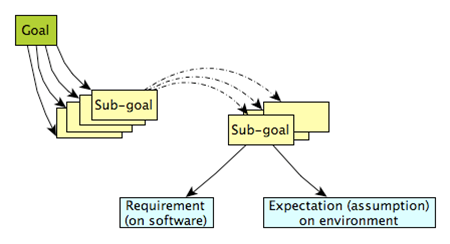
\includegraphics{Forelesning 02/img/3.png}
\caption{Goal refinement}
\end{figure}

Uformelle patterns:

\begin{itemize}
\item
  Achieve{[}TargetCondition{]}
\item
  Cease{[}TargetCondition{]}
\item
  Maintain{[}GoodCondition{]}
\item
  Avoid{[}BadCondition{]}
\item
  Improve{[}TargetCondition{]}
\item
  Increase{[}TargetQuantity{]}
\item
  Reduce{[}TargetQuantity{]}
\item
  Maximise{[}ObjectiveFunction{]}
\item
  Minimise{[}ObjectiveFunction{]}
\end{itemize}
Eksempel:

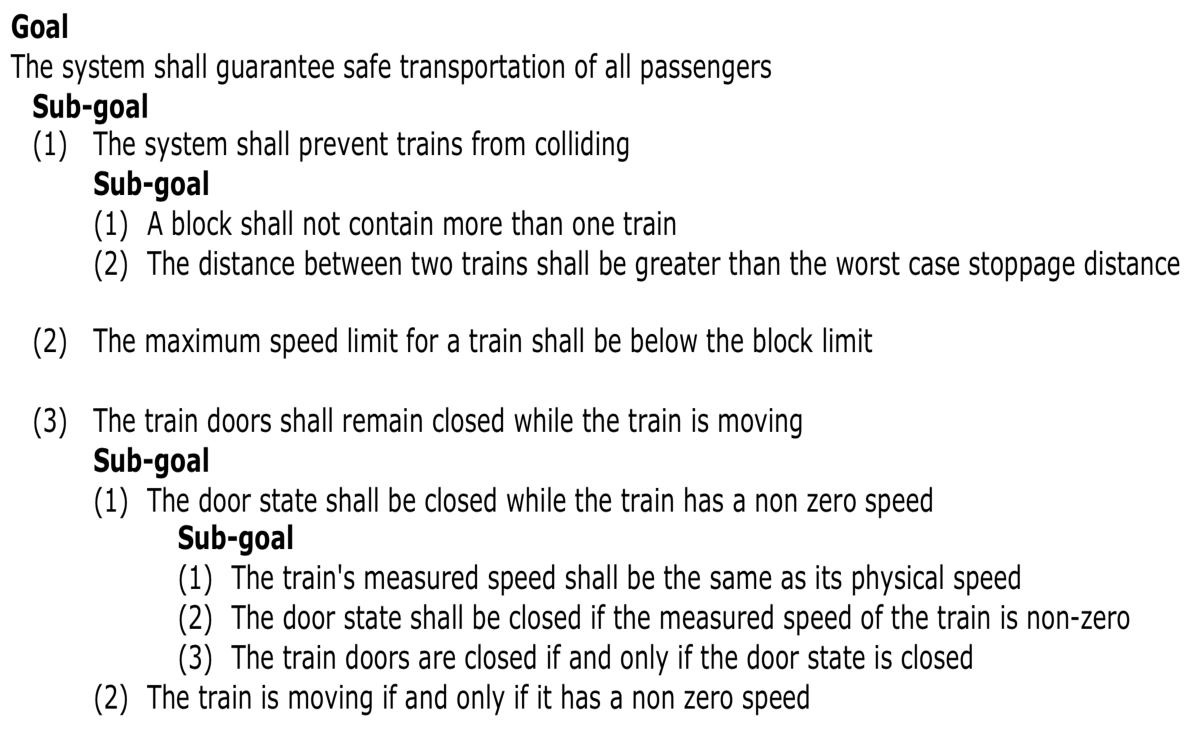
\includegraphics{Forelesning 02/img/refinement-text.PNG}
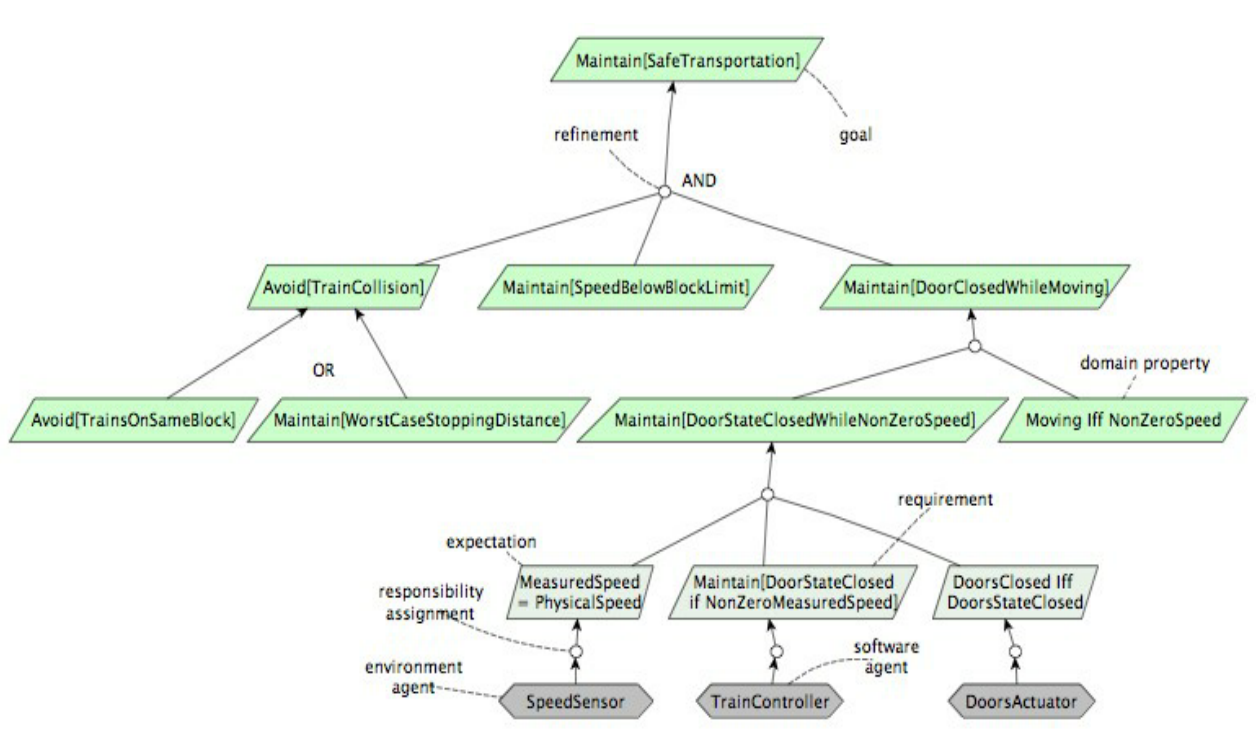
\includegraphics{Forelesning 02/img/refinement-diagram.PNG}
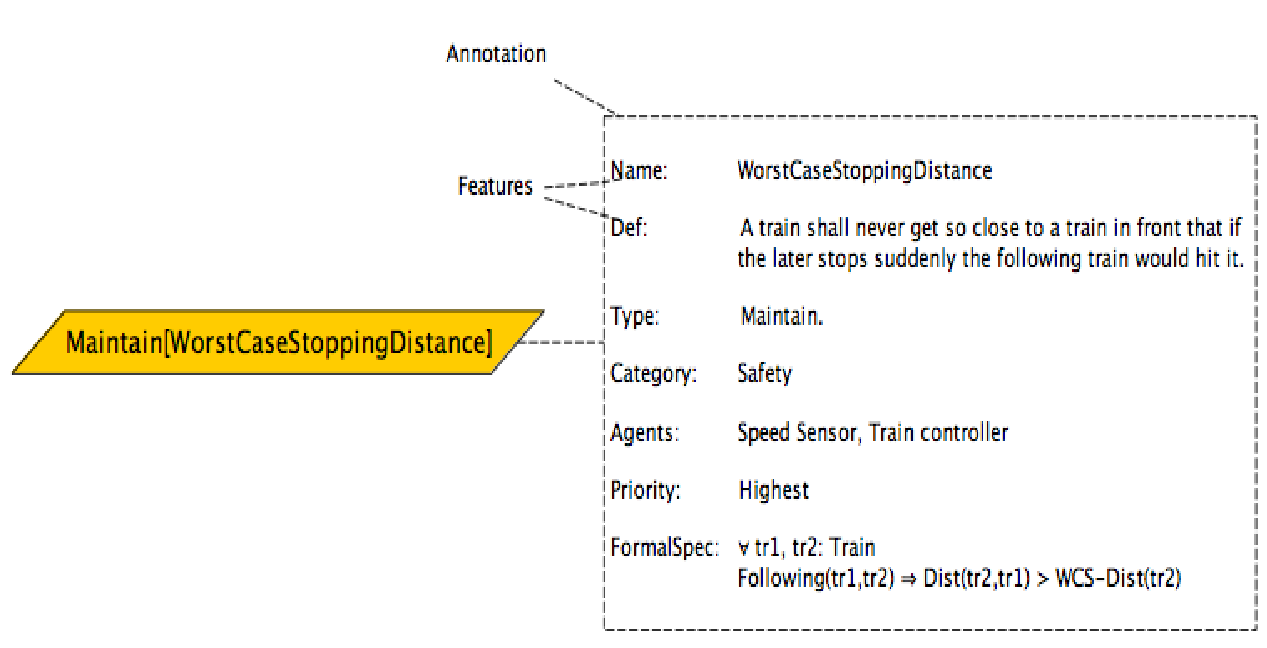
\includegraphics{Forelesning 02/img/refinement-annotation.PNG}

\subsection{Kvalitetsmålprioritet til krav (Quality metrics)}

\begin{itemize}
\item
  Kvalitative mål-krav
  \begin{itemize}
  \item
    Tilnærming til kravspesifikasjon hvor det blir mindre sannsynlig å
    produsere sporinger som er ukonsistente, støyende, ufullstendige
    osv. Se 2-1 for fullstendig oversikt over kvalitetsmålprioritet og
    diagrammer (Ambiguity, inconsistency, forward referencing,opacity,
    noise, completeness).
  \end{itemize}
\item
  Ambiguity
  \begin{itemize}
  \item
    Krav med termer eller utsagn som kan bli tolket på flere måter.
  \end{itemize}
\item
  Inconsistency
  \begin{itemize}
  \item
    Kravsenheter som ikke er kompatible med andre kravsnoder.
  \end{itemize}
\item
  Forward referencing
  \begin{itemize}
  \item
    Kravsenheter som benytter problemverdens-trekk som ikke er definert
    ennå.
  \end{itemize}
\item
  Opacity
  \begin{itemize}
  \item
    Kravsenheter hvor rasjonale eller avhengigheter ikke er synlige
  \end{itemize}
\item
  Noise
  \begin{itemize}
  \item
    Kravsenheter som ikke gir noe informasjon om verdens-trekk.
  \end{itemize}
\item
  Completeness
  \begin{itemize}
  \item
    Behovet til et foreskrevet system er dekket fullstendig av
    kravsenheter uten noen uønskede konsekvenser.
  \end{itemize}
\end{itemize}
\begin{figure}[htbp]
\centering
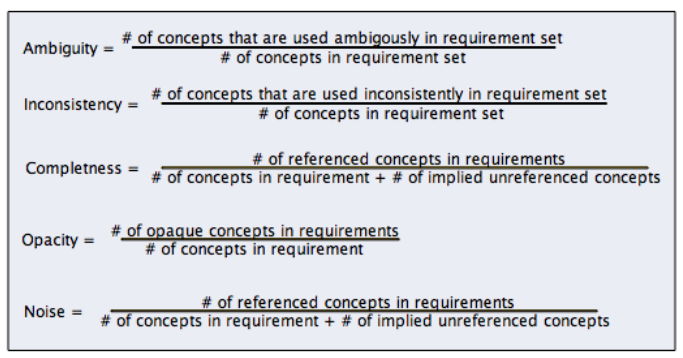
\includegraphics{Forelesning 02/img/quality-metrics.PNG}
\caption{Quality metrics}
\end{figure}

\subsection{Hvor får man mål fra?}

Vi får mål fra preliminære analyser av det nåværende systemet.

\begin{itemize}
\item
  Systematisk ved å søke på nøkkelord i dokumentasjonen vi har
  tilgjengelig, f.eks ``objective'', ``purpose'' osv.
\item
  Iterativ redusering av høynivå mål, ved å spørre \emph{hvordan} og
  \emph{hvorfor}? Gir et goal refinement tree.
\item
  Tilnærming: KAOS - Måldrevet kravinnhenting.
\end{itemize}
\subsection{Oppsummering}

\begin{itemize}
\item
  Mål kan defineres på ulike abstraksjonsnivå.
\item
  To måltyper: Behavioral eller soft goals
\item
  Flere kategorier av mål: Funksjonelle - ikke funksjonelle. Goal
  refinement gir en naturlig mekanisme for å strukturere komplekse
  spesifikasjoner på ulike nivåer (goal refinement tree).
\end{itemize}
\section{2.3 - Guidet naturlig språk (GNL) og Boilerplates (BP)}

Tre nivåer av krav:

\begin{itemize}
\item
  Uformell - Naturlig språk, fri tekst, ingen regler.
\item
  Semiformell
  \begin{itemize}
  \item
    Guided natural language (GNL): fri tekst men tillatte termer er
    definert i et vokabular.
  \item
    Boilerplates (BP): Strukturert tekst og en ontologi. Vokabular +
    relasjoner mellom termer.
  \end{itemize}
\item
  Formell - tilstandsdiagrammer etc.
\end{itemize}
\subsection{Finne krav:}

\begin{enumerate}[1.]
\item
  Finn krav utifra naturlig språk
\item
  Overfør disse kravene til en semi-formell kravmodell
\item
  Avgrens modellen ytterligere for å finne detaljerte krav
\item
  Skap en tidlig designmodell basert på kravene funnet.
\end{enumerate}
Felles for alle stegene er å benytte ordbok med felles vokabular.
Valider og sjekk kravene opp mot konsistens og fullstendighet.

\subsection{Mennesker og Maskiner}

Grunnet høy kompleksitet i requirements engineering, må vi automatisere
så mye som mulig. Mennesker og maskiner har ulike styrker og svakheter.
Vi ønsker derfor å analysere krav på en måte som tillatter begge sider å
bygge på sine sterke sider.

\emph{Maskiner:} God på kvantitative data, raske og presise. God på å
gjøre konsistente repetisjoner. Ikke god på å behandle variasjoner i
skriftlig materiale og mønstergjenkjenning \emph{Mennesker:} God på å
behandle variasjoner i skriftlig materiale. Også god på feilkorrigering.

GNL og BP reduserer variasjon og gir maskinene muligheten til å gjøre
det de kan best: Være raske, presise og konsistente. Ved å kombinere
mennesker og maskiner og la disse gjøre det de kan best, får vi et bedre
resultat. Det endelige målet er å tillate en maskin å assistere
utviklere i analyseringen av krav når det kommer til konsistens,
fullstendighet og sikkerhet.

\subsection{GNL}

Bruker fritekst med assistanse fra et vokabular. Gir oss krav på en
uniform måte for å redusere misforståelser. Altså felles ord alle kan
skjønne. Ingen formelle begrensninger, og krever minimal ekspertise. GNL
prøver å være en mellomting mellom fritekst og mer formelle krav. Måler
kvalitet gjennom korrekthet, konsistens, fullstendighet og redusert
variasjon. GNL er en basis for semantisk prosessering for sjekk av krav.
Bruker en ordbok som kan være en enkel taksonomi eller mer formell
ontologi.

\emph{Ontologi} : Thesaurus (Domenekonsepter som entiteter, termer og
hendelser) + inferensregler (Relasjoner, attributter og aksiomer).

Fange kunnskap gjennom informasjon fra domeneeksperter. Implementer
denne kunnskapen gjennom f.eks OWL, og verktøy som Protege. Verifiser at
ontologien er korrekt.

\subsubsection{Boilerplates}

Tekst har fordelen med at den ikke er begrenset av noe, men man trenger
en felles forståelse av konseptene som blir brukt for å uttrykke kravene
og relasjonene mellom dem - altså hvordan dette presenteres.
Boilerplates, eller såkalt ``template based textual requirements
specification'' gir noen begrensninger for å redusere sjansen for
ukonsistente uttrykk.

\emph{Boilerplate} : En basis for sjekking av krav. Enkle å forstå for
interessenter i forhold til mer formelle representasjoner. BP kan brukes
til både funksjonelle og ikke funksjonelle krav.

\begin{figure}[htbp]
\centering
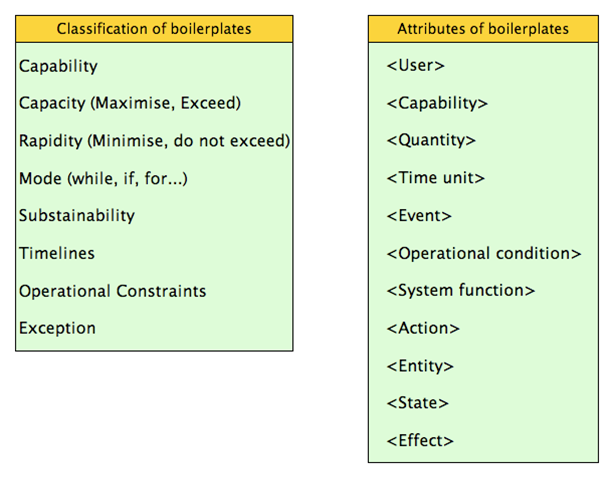
\includegraphics{Forelesning 02/img/1.png}
\caption{Boilerplates}
\end{figure}

\paragraph{RE-Prosessen:}

En boilerplate består av faste termer og attributter. Den kan, men må
ikke, ha en eller flere modi (modes).

\begin{enumerate}[1.]
\item
  Velg en boilerplate eller en sekvens med disse. Seleksjonen er basert
  på attributtene som må inkluderes og hvordan de er organisert -
  \emph{faste termer} .
\item
  Hvis nødvendig, identifiser og inkluder \emph{mode} boilerplates
\item
  Instansier alle attributter
\end{enumerate}
Typisk boilerplate-eksempel:

\textbf{BP32}: The \texttt{\textless{}user\textgreater{}} shall be able
to \texttt{\textless{}capability\textgreater{}}.

\textbf{Attributtene}: \texttt{\textless{}user\textgreater{}} = driver
og \texttt{\textless{}capability\textgreater{}} = starte ACC systemet.

Kravet blir da: \emph{The \textbf{driver} shall be able to \textbf{start
the ACC system}.}

\begin{itemize}
\item
  Mode
  \begin{itemize}
  \item
    while
  \item
    if
  \item
    within
  \item
    without
  \item
    from
  \item
    for
  \item
    in
  \item
    between
  \item
    after
  \item
    before
  \item
    when
  \end{itemize}
\item
  FixedTerm
  \begin{itemize}
  \item
    shall be able to
  \item
    at a minimum rate og
  \item
    times per
  \item
    for a period of at least
  \item
    shall allow
  \item
    shall not
  \item
    except for
  \item
    without affecting
  \item
    may be
  \item
    shall be
  \item
    other than
  \item
    to be
  \item
    to
  \item
    get
  \item
    shall
  \end{itemize}
\item
  Attributes
  \begin{itemize}
  \item
    User
  \item
    Entity
  \item
    Capability
  \item
    Quantity
  \item
    Time unit
  \item
    Event
  \item
    Operational condition
  \item
    System
  \item
    Action
  \item
    State
  \item
    Object
  \item
    Unit
  \end{itemize}
\end{itemize}
\begin{quote}
\emph{The \textbf{weapons operator} shall be able to \textbf{fire a
missile} within \textbf{3 seconds} of \textbf{radar sighting} while
\textbf{in severe sea conditions}}

\end{quote}
Det er med andre ord en måte å skrive om interessenter i en situasjon i
et domene. \textbf{The language of requirements}.

\begin{figure}[htbp]
\centering
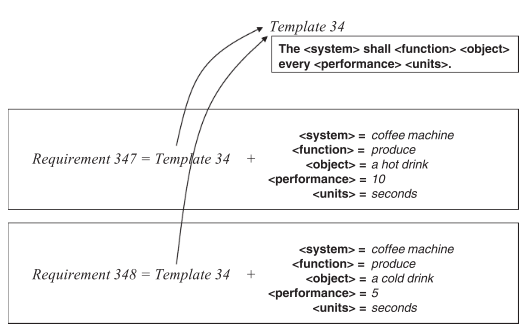
\includegraphics{Forelesning 02/img/boilerplate.png}
\caption{}
\end{figure}

\subsection{Oppsummering}

Ved å bruke boilerplates og ontologier får vi:

\begin{itemize}
\item
  En felles bruk av termer, og reduserer variasjonen av mulige
  presentasjoner. Krav som er like skal se like ut.
\item
  Redusert variasjon i form og innhold som forenkler bruken av
  automatiserte og semiautomatiserte verktøy for å sjekke kvalitet
  (completeness, consistency) og lage test cases.
\end{itemize}
\section{11.2 - Smidige krav gjennom brukerhistorier og -scenarioer}

Hovedprinsippene bak smidige krav er:

\begin{itemize}
\item
  Aktiv brukerinvolvering
\item
  Smidige team må ha mulighet til å gjøre valg
\item
  Krav dukker opp og utvikler seg sammen med programvaren som utvikles
\item
  Smidige krav er ``såvidt tilstrekkelige''
\item
  Krav utvikles i små deler
\item
  Nok er nok -- bruk 80/20-regelen
\item
  Samarbeid, samhandling og kommunikasjon mellom alle teammedlemmer er
  helt essensielt
\end{itemize}
Skriftlige krav er godt uttenkte, gjennomgåtte og redigerte. Varige.
Enkelt å dele i grupper mennesker. Skriftlige krav tar imidlertid mye
tid å produsere, kan bli mindre relevante over tid, og kan enkelt
misforståes.

Mintlige krav gir en mulighet til øyeblikkelig tilbakemelding og
avklaring, noe som kan gi en bedre felles forståelse.
Informasjonsutvekslingen er fylt med informasjon. Når ny informasjon
kommer er det mulighet for å bedre kunne justere krav. Kan utløse ideer
om problemer og muligheter.

\subsection{Brukerhistorier}

\begin{quote}
User stories seek to combine the strengths of written and verbal
communication, where possible suppoted by a picture. -- Kent Beck

\end{quote}
En brukerhistorier er en tekstlig beskrivelse av en hypotetisk bruker av
systemet. Disse historiene beskriver og består av brukerens behov,
beskrivelse av produktet, planleggingsenheter, tegn for samtale og
mekanismer for samtaleutsettelse.

En brukerhistorie består av tre deler: en \emph{beskrivelse}, en
\emph{samtale} og en \emph{bekreftelse}. Beskrivelsen er en tekstlig
beskrivelse av brukerhistorien for bruk til planlegging og som en
``huskelapp''. Samtalen er en seksjon som skal fange opp mer informasjon
om brukerhistoren og alle samtalers detaljer. Bekreftelsen er en sekjson
dedikert til å formidle de tester som skal utføres for å bekrefte at
brukerhistorie er komplett og fungerer som forventet.

\subsubsection{Hvordan skrive en brukerhistorie}

Det en trenger for å skrive en brukerhistorie er \emph{hvem} (brukerens
rolle), \emph{hva} (et mål) og \emph{hvorfor} (et rasjonale). Dette
bidrar til å avklare hvorfor en funksjon er nyttig, kan påvirke en
funksjons funksjon samt gi en gode ideer for andre nyttige funksjoner
som kan bidra til å støtte brukerens mål.

As a {[}user role{]} I want to {[}goal{]} so I can {[}reason{]}.

As a \emph{registered user} I want to \emph{log in} so I can
\emph{access subscriber-only content}.

\begin{enumerate}[1.]
\item
  Start med en tittel
\item
  Legg ved en konsis beskrivelse ved å bruke ovenstående templates
\item
  Legg ved andre relevante notater, spesifikasjoner og skisser
\item
  Skriv akseptansekriterier \emph{før programvaren bygges}
\end{enumerate}
En brukerhistorie er detaljert nok når den gjør teamet i stand til å
starte arbeidet sitt, og etablerer flere detaljer og avklaringer ved
utviklingstid.

Huskeregel: INVEST

\begin{itemize}
\item
  Independent - bør være så uavhengige av hverandre som mulig
\item
  Negotiable - må være mulig å forhandle i løpet av planleggingsfasen
\item
  Valuable - må være verdifulle for brukeren, skrives på brukerens
  språk, funksjoner ikke oppgaver
\item
  Estimatable - må være mulig å estimere, må inneholde nok informasjon
  (men ikke for mye)
\item
  Small - må være liten (men ikke for liten)
\item
  Testable - må være skrevet slik at den er testbar
\end{itemize}
Brukerhistorier prioriteres i en \emph{backlog} slik at de mest
verdifulle oppføringene har høyest prioritet. Den samlede massen
prioriterte brukerhistorier kalles en \emph{produkt-backlog}.

\subsubsection{User story mapping}

En tilnærming for organisering og prioritering av brukerhistorier er
\emph{user story mapping}. Her vil en gjøre arbeidsflyten og verdikjeden
synlig, vise relasjonen mellom større historier og deres barn, hjelpe
til med å bekrefte backloggens fullstendighet, gi en nyttig
prioriteringskontekst, planlegge utgivelser i komplette og verdifulle
stykker funksjonalitet.

Her vil en arrangere aktiviteter og oppgavesentrerte historiekort romlig
(spatially) for å kunne identifisere større historier. En legger ut
disse kortene, fra venstre mot høyre, i den rekkefølgen en ville
forklart de til en person som spør: Hva vil mennesker gjøre med
systemet.

\begin{figure}[htbp]
\centering
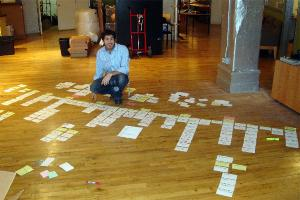
\includegraphics{Forelesning 11/img/large-floor-map.jpg}
\caption{}
\end{figure}

Brukeroppgaver overlappe vertikalt om en bruker vil kunne utføre en
oppgave mer eller mindre på samme tid (tenk: flere funksjoner på én
side). ``Huskeregelen'' her er at om en bruker ``gjør X eller Y eller Z,
deretter P'', vil aller tilfeller av ``eller'' være en vertikal
stabling, ``deretter'' er horisontal.

Det resulterende kartet viser en dekomponering og typisk flyt gjennom
hele systemet. Gjennom å lese aktivitetene over systemets topp vil en
kunne bedre forstå end-to-end-bruken av systemet.
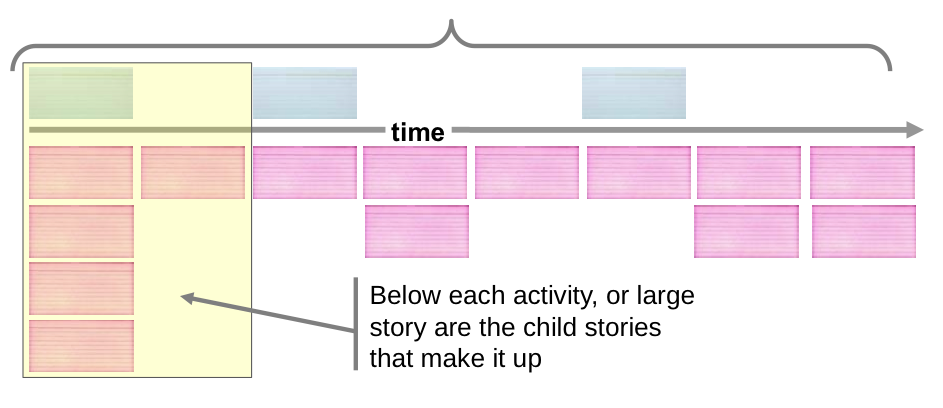
\includegraphics{Forelesning 11/img/2.png}

Videre vil en prioritere disse historiene basert på produktets mål.
Dette målet beskriver utfallet eller nytten en organisasjon vil ha av å
bruke produktet. Disse målene kan videre identifisere potensielle
inkrementelle utgivelser, hvor hver enkelt utgivelse gir en form for
nytte.

Del opp kartet inn i lag for å gruppere funksjoner inn i utgivelser.
Arrangere så funksjonene vertikalt basert på nytte sett fra brukerens
perspektiv. Del oppgaver inn i deler som kan utsettes til senere
utgivelser. Benytt deretter produktmålene for å identifisere stykker som
inkrementelt realiserer disse.

\begin{figure}[htbp]
\centering
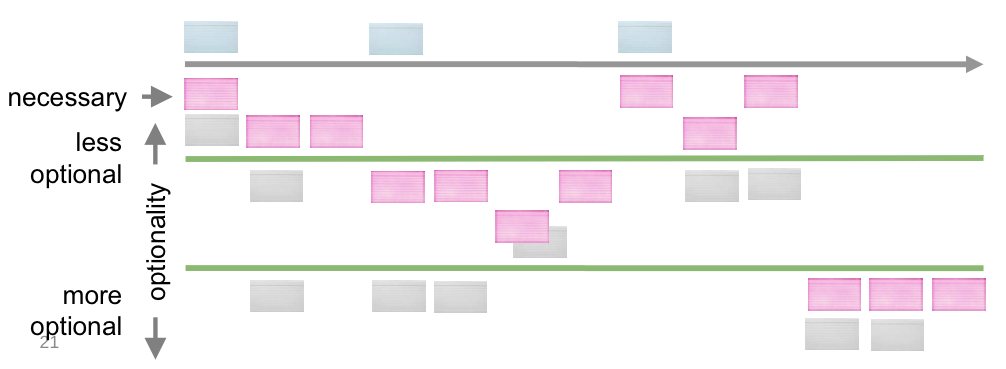
\includegraphics{Forelesning 11/img/3.png}
\caption{}
\end{figure}

\subsection{Fra brukerhistorie til test-case}

\subsection{CUCUMBER}

\begin{itemize}
\item
  Scenario - kort beskrivelse av testscenario
\item
  Given - forutsetninger for testen
\item
  When - input
\item
  Then - output
\item
  And - kan brukes for å inkludere mer enn én forutsetning, input eller
  output
\end{itemize}
\subsubsection{Eksempel}

\begin{itemize}
\item
  Scenarion - memory BIT
\item
  When - we have inserted a memory fault
\item
  And - run a memory BIT
\item
  Then - the memory fault flag should be set
\item
  And - the system should move to the error state
\end{itemize}
\subsection{Utfordringer ved bruk av smidige krav}

Aktive brukere kan være krevende, basert på brukerrepresentaters to.
Krever og en mye forpliktelse gjennom hele prosjektets varighet.

Iterasjoner kan bidra til betydelig overhead dersom utgivelseskostnader
er høye.

Smidige krav er så vidt tilstrekkelige som betyr at mindre informasjon
tilgjengelig for nybegynnere i teamet om funksjoner og hvordan de skal
fungere. (wut?)

Som regel vil ikke smidige krav være passende for prosjekter med høy
utvklingsturnover med langtids-vedlikeholdskontrakter.

Ikke passende for sikkerhetskritiske systemer.

\subsection{Oppsummering}

\begin{itemize}
\item
  Brukerhistorier kombinerer skriftlig og verbal kommunikasjon,
  understøttet med bilde hvor det er mulig
\item
  Brukerhistorer bør beskrive funksjoner som er av verdi til brukeren,
  skrevet på brukerens språk
\item
  Brukerhistorer gir tilstrekkelig informasjon, men ikke mer
\item
  Detaljer utsettes og samles opp gjennom samhandling JIT for utvikling
\item
  Test-cases bør skrives før utviklingen starter, etter en
  brukerhistorie er skrevet
\item
  Brukerhistorer bør være Independent, Negotiable, Valuable,
  Estimatable, Small og Testable.
\end{itemize}
\subsection{Nyttige URLer}

\href{http://www.agileproductdesign.com/presentations/user\_story\_mapping/index.html}{User
story mapping}

\section{11.2 - Advanced Use cases}

Aktør : Eksterne parter som interagerer med systemet. Har en
\emph{rolle} (tilsvarer \emph{ikke} jobbtittel). Denne rollen
responderer til systemets spørringer. : En aktør behøver ikke være en
person -- det kan være et system eller et subsystem.

Use Case : En sekvens av handlinger som systemet utfører som resulterer
i et observerbart resultat av en verdi til en aktør-

Use Case Model : Inneholder en aktørliste, pakker, diagrammer, use-cases
og views. : Inkluderer strukturererte use-case-beskrivelse som er
forankret i veldefinerte konsepter begrenset av krav og omfang.

\subsection{Hvordan finne aktører}

Viktige spørsmål en må spørre seg når en skal finne potensielle aktører
er:

\begin{itemize}
\item
  Hvem bruker systemet?
\item
  Hvem får informasjon fra systemet?
\item
  Hvem gir informasjon til systemet?
\item
  Hvilke andre systemer benytter seg av systemet?
\item
  Hvem installerer, starter eller vedlikeholder systemet?
\end{itemize}
Ha først fokus på menneskelige og andre primæraktører. Grupper så
individer etter felles oppgaver og systembruk -- navngi og definér deres
felles roller. Identifisér systemer som initierer interaksjoner med
systemet, samt andre systemer som brukes for å utføre systemets
oppgaver.

\subsection{Hvordan finne use-cases}

\begin{itemize}
\item
  Beskrive de funksjoner brukerer ønsker fra systemet.
\item
  Beskrive alle CRUD-operasjoner (operasjoner som skaper, leser,
  oppdaterer og sletter informasjon)
\item
  Beskrive hvordan aktører varsles om endringer til den systemets
  interne tilstand.
\item
  Beskrive hvordan aktører kommuniserer informasjon om hendelser som
  systemet må vite om.
\end{itemize}
Det å skape use-cases er en iterativ prosess hvor en involverer
interessenter i hver operasjon. Det er svært sjeldent en klarer å skape
de perfekte use-caser på første forsøk.

Det er vanlig å bruke UML-notasjon.

\begin{enumerate}[1.]
\item
  Definér aktører
  \begin{itemize}
  \item
    Husk at også systemer kan definerers som aktører
  \item
    Ta også meg abuse-agenter
  \end{itemize}
\item
  Definér nøkkelaktører
\item
  Definér use-cases for nøkkelaktørenes mål
\item
  Abstraher og gjenbruk av generiske handlinger som spesielle aktører
  kan arve handlinger fra.
  \begin{itemize}
  \item
    Dependency (``Gjør en betaling'' er avhengig av at ``Logg inn'' er
    utført)
  \item
    Include (``Utfør en betaling'' inkluderer ``Validere midlers
    tilgjengelighet'')
  \item
    Extends (``Gjør en periodisk betaling'' og ``Gjør en enkel
    betaling'' extender ``Gjør en betaling'')
  \item
    Generalize
  \end{itemize}
\item
  Legg til detaljer som \emph{boundary object}, \emph{control object} og
  \emph{entity object}.
\end{enumerate}
!{[}Abstrahering av en generisk bruker{]}Forelesning 11/img/1.png)

Konvertering til sekvensdiagram

\subsection{Use case index}

Hvert use-case har flere attributter som relatererer til seg selv og til
prosjektet. På prosjektnivå vil disse attributtene inkludere omfang,
kompleksitet, status og prioritet

\ctable[pos = H, center, botcap]{llllll}
{% notes
}
{% rows
\FL
\parbox[b]{0.17\columnwidth}{\raggedright
\emph{Use Case ID}
} & \parbox[b]{0.21\columnwidth}{\raggedright
\emph{Use Case Name}
} & \parbox[b]{0.21\columnwidth}{\raggedright
\emph{Primary Actor}
} & \parbox[b]{0.13\columnwidth}{\raggedright
\emph{Scope}
} & \parbox[b]{0.17\columnwidth}{\raggedright
\emph{Complexity}
} & \parbox[b]{0.12\columnwidth}{\raggedright
\emph{Priority}
}
\ML
\parbox[t]{0.17\columnwidth}{\raggedright
1
} & \parbox[t]{0.21\columnwidth}{\raggedright
Places a bid
} & \parbox[t]{0.21\columnwidth}{\raggedright
Buyer
} & \parbox[t]{0.13\columnwidth}{\raggedright
In
} & \parbox[t]{0.17\columnwidth}{\raggedright
High
} & \parbox[t]{0.12\columnwidth}{\raggedright
1
}
\\\noalign{\medskip}
\parbox[t]{0.17\columnwidth}{\raggedright
2
} & \parbox[t]{0.21\columnwidth}{\raggedright
Purchases an item
} & \parbox[t]{0.21\columnwidth}{\raggedright
Buyer
} & \parbox[t]{0.13\columnwidth}{\raggedright
In
} & \parbox[t]{0.17\columnwidth}{\raggedright
High
} & \parbox[t]{0.12\columnwidth}{\raggedright
1
}
\\\noalign{\medskip}
\parbox[t]{0.17\columnwidth}{\raggedright
3
} & \parbox[t]{0.21\columnwidth}{\raggedright
Creates account
} & \parbox[t]{0.21\columnwidth}{\raggedright
Generic User
} & \parbox[t]{0.13\columnwidth}{\raggedright
In
} & \parbox[t]{0.17\columnwidth}{\raggedright
Med
} & \parbox[t]{0.12\columnwidth}{\raggedright
1
}
\\\noalign{\medskip}
\parbox[t]{0.17\columnwidth}{\raggedright
4
} & \parbox[t]{0.21\columnwidth}{\raggedright
Searches listings
} & \parbox[t]{0.21\columnwidth}{\raggedright
Generic User
} & \parbox[t]{0.13\columnwidth}{\raggedright
In
} & \parbox[t]{0.17\columnwidth}{\raggedright
Med
} & \parbox[t]{0.12\columnwidth}{\raggedright
1
}
\\\noalign{\medskip}
\parbox[t]{0.17\columnwidth}{\raggedright
5
} & \parbox[t]{0.21\columnwidth}{\raggedright
Provides feedback
} & \parbox[t]{0.21\columnwidth}{\raggedright
Generic User
} & \parbox[t]{0.13\columnwidth}{\raggedright
In
} & \parbox[t]{0.17\columnwidth}{\raggedright
High
} & \parbox[t]{0.12\columnwidth}{\raggedright
1
}
\\\noalign{\medskip}
\parbox[t]{0.17\columnwidth}{\raggedright
6
} & \parbox[t]{0.21\columnwidth}{\raggedright
Creates an auction
} & \parbox[t]{0.21\columnwidth}{\raggedright
Seller
} & \parbox[t]{0.13\columnwidth}{\raggedright
In
} & \parbox[t]{0.17\columnwidth}{\raggedright
High
} & \parbox[t]{0.12\columnwidth}{\raggedright
1
}
\\\noalign{\medskip}
\parbox[t]{0.17\columnwidth}{\raggedright
7
} & \parbox[t]{0.21\columnwidth}{\raggedright
Ships an item
} & \parbox[t]{0.21\columnwidth}{\raggedright
Seller
} & \parbox[t]{0.13\columnwidth}{\raggedright
In
} & \parbox[t]{0.17\columnwidth}{\raggedright
High
} & \parbox[t]{0.12\columnwidth}{\raggedright
2
}
\LL
}

Use-case-diagrammer er som regel lette å forstå og enkle å tegne. Mer
komplekse diagrammer, av typen som bruker \textless{}\textgreater{} og
\textless{}\textgreater{} kan være noe vanskeligere å forstå. Et
use-case-diagram forteller heller ikke noe om en handlings sekvens.

\subsection{Tekstlige use-cases}

Use-case-element
Beskrivelse
Use-case-nummer
ID som representerer use-caset
Applikasjon
Systemet eller applikasjonen denne hører til
Use-case-navn
Use-casets navn. Hold det konsist.
Beskrivelse
Utbrodere navnet, litt mer fyldig.
Primæraktør
Hovedaktøren som dette use-caset representerer
Forutsetning
Forutsetninger som må være tilstede for at dette use-caset kan starte
Trigger
Det som trigger dette use-caset
Grunnleggende flyt
Perfekt gjennomføring, uten feil.
Alternativ flyt
De mest signifikante alternativer og unntak fra den grunnleggende flyten
Eksempler på alternativ flyt involverer at en kundes kredittkort ikke
godkjennes, session timeout. Alternativ flyt kan håndteres av
\textless{}\textgreater{} og \textless{}\textgreater{}.

Sette inn eksempler her? Bah, mer tabeller :/

Komplekse tekstlige use-cases er enklere å forstå enn komplese
UMl-diagrammer, og kan og være enklere å oversette til sekvensdiagrammer
da de viser sekvensen til en handling. På den andre siden tar de mer
tidkrevende å produsere.

\subsection{Mis-Use cases}

Brukes for å identifisere mulige misuses av systemet. Brukes på samme
måte som et ordinært use-case, men med markerte fiendtlige aktører.
Angrepsvektorer markeres og med \emph{threatens} fra fiendtlig handling
til ordinær handling. Fiendtlige aktører kan være på grunn av
utilsiktede feil fra ordinære brukere og fra kuk i computeren.

UC-name
Respond to over-pressure
User action
System response
Threats
Mitigations
Alarm operator o high pressure
System fails to set alarm; Operator fails to notice alarm
Have two independent alarms; Test alarms regularly; Use both audio and
visual cues; Alarm also outside control room
Operator gives command to empty tank
Operator fails to react (e.g.~ill, unconsious); Operator gives wrong
command (e.g.~filling tank)
Alarm backup operator; Automatic sanity check; Diallow filling at high
pressure
System opens valve to sewer
System fails to relay command to valve; Valve is stuck
Operator reads pressure
Operator misreads and stops emptying too soon
Maintain alarm until situation is normal
\subsubsection{Hvorfor misuse case?}

Et misuse-case brukes på tre måter:

\begin{itemize}
\item
  Identifisering av trusler
\item
  Identifisering av nye krav
\item
  Identifisering av nye tester
\end{itemize}
Fordeler med misuse-cases inkluderer muligheten til å fokusere på mulige
problemer, og å se på mulige forsvars- og mitigasjonsstrategier.
Misusediagrammer kan bli noe komplekse.

\subsection{Use-case maps}

Use case map : En visuell representasjon av et systems krav ved å bruke
er presist definert sett av symboler for ansvar, systemkomponenter og
sekvenser. : Lenker sammen oppførsel og struktur på en eksplisitt og
visuell måte.

Use case map path : Arkitekturiske entiteter som beskriver uformell
relasjon mellom ansvar, som bundet til underliggende organisatoriske
strukturer av abstrakte komponenter. : Brukes for å skape en kobling
mellom krav og detaljert design.

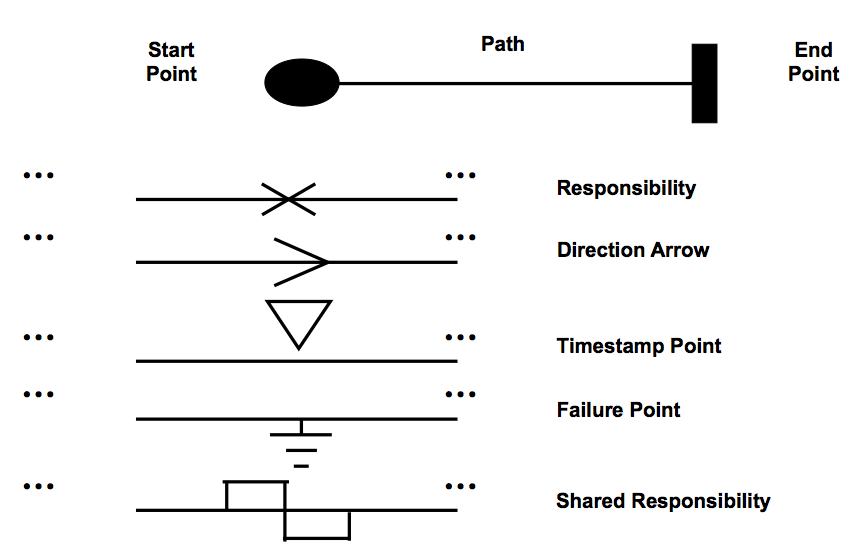
\includegraphics{Forelesning 11/img/ucm-path.png}
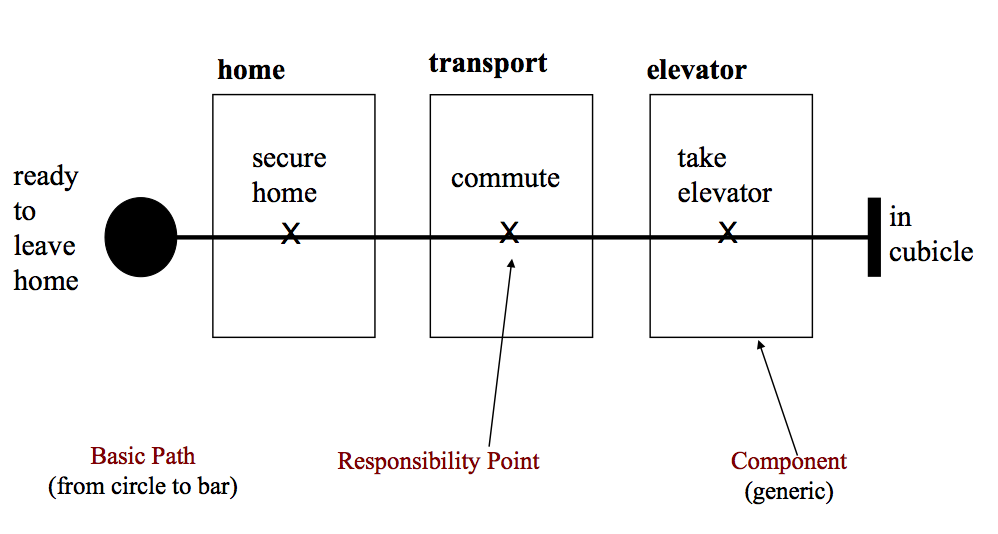
\includegraphics{Forelesning 11/img/ucm-path-example.png}
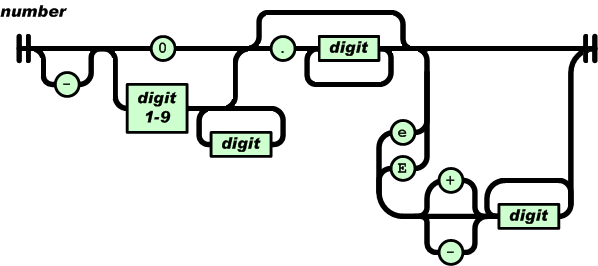
\includegraphics{Forelesning 11/img/number.png}
\href{http://cukes.info/}{Cucumber -- Cucumber testing}

\ldots{} cue eksempler i massemassevis

Hohoy denne notasjonen var full av fuck

\section{5.1 - Test vs.~inspection}

Noen defekter er viktige ettersom de oppstår ofte. De fleste defekter er
derimot mindre viktige, da de oppstår sjeldent. Problemet er å skille
disse to tilfellene fra hverandre. Hvordan gjør en det mest effektivt og
så nøyaktig som mulig?

Testing kan ikke alltid gjøres -- til å begynne med har en ikke kode å
teste med. Vi må derfor utføre ulike typer inspeksjoner. Dette er en av
de største svakhetene med tradisjonell utvikling kontra smidig
utvikling.

\subsection{Fit's List}

\begin{figure}[htbp]
\centering
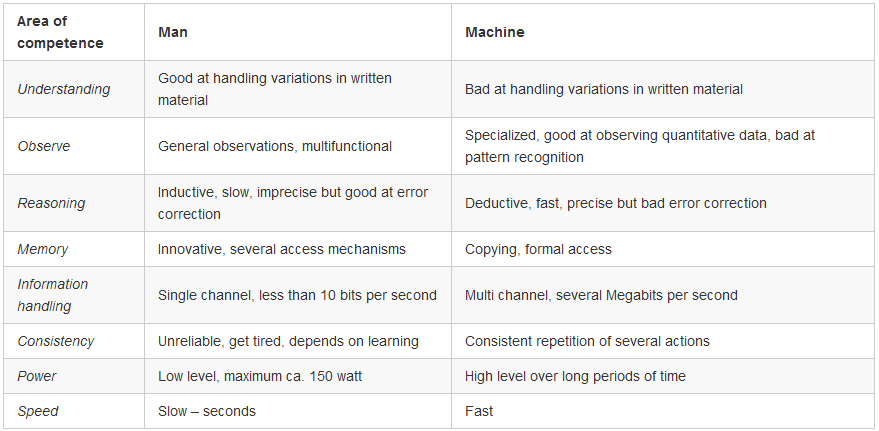
\includegraphics{Forelesning 05/img/3.png}
\caption{}
\end{figure}

Et menneske er derfor bra når en behøver en evne til å håndtere varierte
situasjoner, være innovativ og induktiv, samt når en vil gjenkjenne
mønstre. Mennesker er på den andre siden mindre gode til å gjøre det
samme om og om igjen på en konsistent måte. Dette gjør at menneskelig
behanding av store datamengder ikke er å anbefale. Til slikt benytter en
seg av maskiner. Menneske og maskin utfyller hverandre ved å utnytte
hverandres styrker, ved at maskinen hjelper mennesket å håndtere store
mengder informasjon, og mennesket hjelper maskinen ved å gi den
innovative inndata.

\subsection{Generell konsiderasjon}

\subsubsection{Dokumenter}

Design av arkitektur, system, sub-system og komponenter, samt
pseudo-kode er eksempler på \emph{dokumenter}, områder hvor tester enten
ikke fungerer i det hele tatt, eller fungerer mindre bra. Her bør vi kun
benytte oss av inspeksjoner.

Mennesker bruker sin erfaring og kunnskap til å identifisere mulige
problemer, maskinen tilbyr støtte via å identifisere relevant
informasjon.

\subsubsection{Kode}

For eksekvérbar kode kan en benytte seg av inspeksjon, testing eller en
kombinasjon av begge disse, avhengig av kodens størrelse og
kompleksitet. Andre viktige faktorer som farger valget av inspeksjon og
test er programmeringsspråket og algoritmer som brukes for
realiseringen.

En generell regel er at om en står overfor en tilstrekkelig liten
kodebase vil en kunne utføre inspeksjon av hele denne basen, for så å
designe og utføre tester på bakgrunn av funnene her. I tilfelle kompleks
kode, vil en og starte med inspeksjon av koden, men her vil en fokusere
på algoritmer og logikk. Da en i slike tilfeller ikke kan teste
\emph{hele} kodebasen, vil en måtte utforme kompletthetskriterer for
testene, som deretter designes og kjøres.

Kompletthetskriterier : SOMETHING

\subsection{Inspeksjonsprosesser}

For alle inspeksjonstyper - GIGO. Det kan og være en god idé å involvere
kunderepresentanter.

\hyperdef{}{walkthrough}{\subsubsection{Walkthrough}\label{walkthrough}}

Intern. Bukes for tidlig beslutningstaking.

\begin{enumerate}[1.]
\item
  Skape en grov skisse av løsningen
  \begin{itemize}
  \item
    Arkitektur, algoritme, etc.
  \end{itemize}
\item
  Presentering
  \begin{itemize}
  \item
    Forklare skissen til oppmøtte
  \end{itemize}
\item
  Registrering av feeback og komme med forslag til forbedringer.
\end{enumerate}
\paragraph{Fordeler}

Fordeler med walkthrough av koden inkluderer at den er både enkel og
billig. Dette muliggjør at en kan samle ideer på et tidlig stadie i
utviklingen.

\paragraph{Ulemper}

Ulemper er at da prosessen er uformell er der ingen forpliktelser hos
deltakerne. Prosessen skaper og mange løse og irrelevante ideer.

\subsubsection{Uformell inspeksjon}

Intern.

\begin{figure}[htbp]
\centering
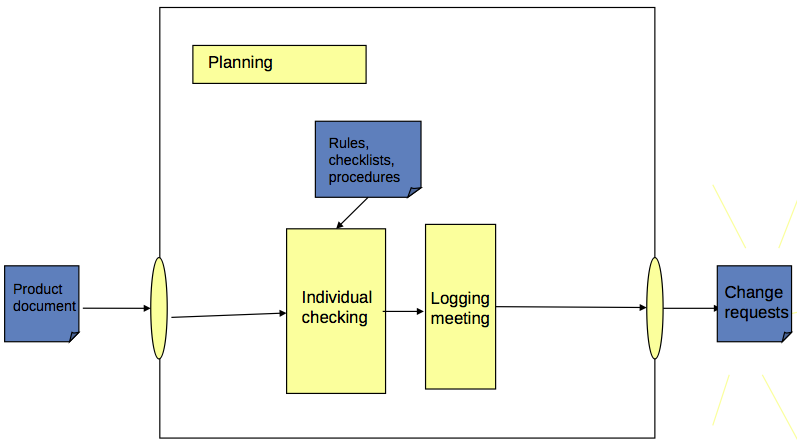
\includegraphics{Forelesning 05/img/1.png}
\caption{Uformell inspeksjon}
\end{figure}

\paragraph{Fordeler}

\begin{itemize}
\item
  Enkel og billig å gjennomføre
\item
  Kan uføres i alle av utviklingens stadier
\item
  Har som regel en god kostnad/nytte-ratio
\item
  Krever kun et minimumsnivå av planlegging
\end{itemize}
\paragraph{Ulemper}

Som ved bruk av \href{\#walkthrough}{walkthrough} vil det ikke være en
formell forpliktelse blant deltakerne. En plukker heller ikke opp
potensielle prosessforbedringer.

\subsubsection{Formell inspeksjon}

Formell inspeksjon anbefales å være en del av den endelige
akseptansetestingen av viktige dokumenter.

Som utredet av
\href{http://books.google.no/books?id=GO11btO0-vIC\&q=\%22software+inspection\%22\&dq=\%22software+inspection\%22\&hl=en\&sa=X\&ei=KNZ1T\_WcKeL64QSn99mbDw\&redir\_esc=y}{T.
Gilb og D. Graham}

\begin{figure}[htbp]
\centering
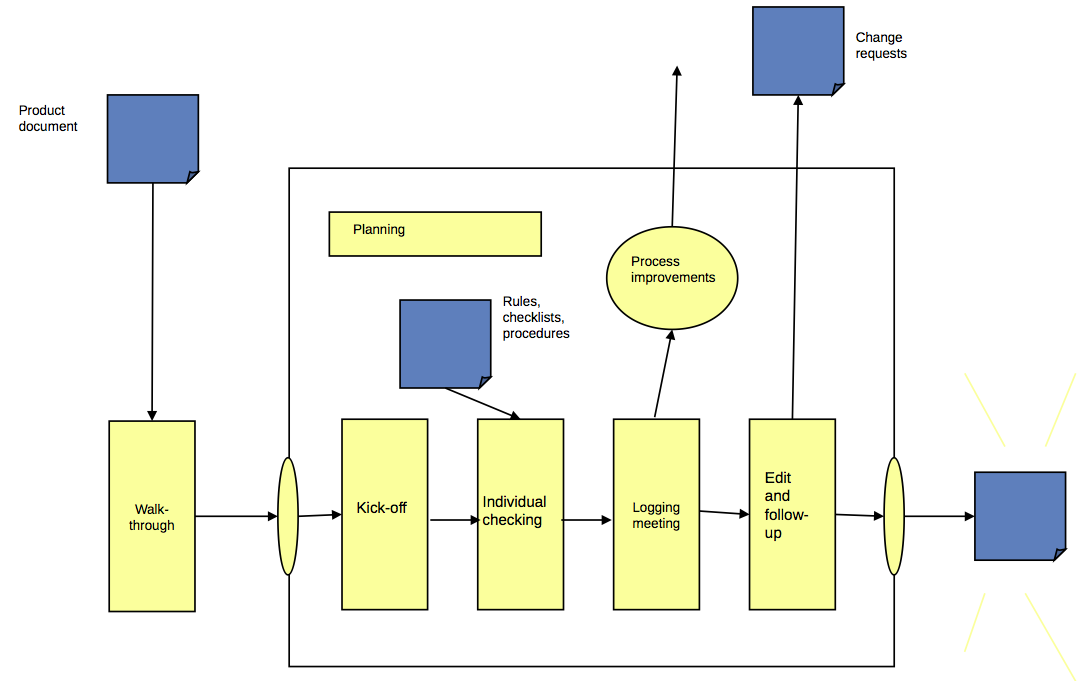
\includegraphics{Forelesning 05/img/2.png}
\caption{Formell inspeksjon}
\end{figure}

\paragraph{Distribusjon av resusser}

\begin{figure}[htbp]
\centering
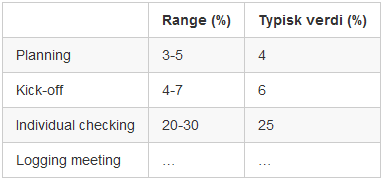
\includegraphics{Forelesning 05/img/4.PNG}
\caption{}
\end{figure}

(TODO: Resten av slide 24 har falt bort)

\paragraph{Initiering av inspeksjonsprosessen}

Inspeksjonsprosessen starter ved at forfatter sender en
inspeksjonsforespørsel til QA-ansvarlig. Dersom dokumentet defineres å
være klar for inspeksjon vil så QA-ansvarlig utnevne en
inspeksjonsleder.

\paragraph{Planlegging}

Viktige momenter som planlegging skal besvare er \emph{hvem som skal
delta i inspeksjonen}. De som skal delta bør ha interesse, tid og den
kunnskapen som behøves for å sette seg inn i inspeksjonen.

\paragraph{Kick-off}

\begin{itemize}
\item
  Distribuering av nødvendige dokumenter
\item
  Tildeling av inspeksjonsspesifikke roller og jobber
\item
  Sette mål for resursser, deadlines, etc.
\end{itemize}
\paragraph{Individuell kontroll}

Den individuelle kontrollen er inspeksjonens hovedaktivitet. Her vil
hver enkelt deltaker lese gjennom dokumentet for å se etter
\emph{potensielle feil} -- det vil si inkonistens i forhold til krav
eller total applikasjonsfølelse, eller \emph{mangel på etterlevelse} i
forhold til selskapet standarder eller godt håndtverk.

\paragraph{Loggføring av møtet}

\begin{itemize}
\item
  Loggføring av \emph{saker} allerede funnet av inspeksjonens deltakere.
\item
  Finne \emph{nye} saker, basert på diskusjoner og ny informasjon som
  dukker opp under loggføringen av møtet.
\item
  Identifisering av mulige forbedringer av inspeksjons- eller
  utviklingsprosessen.
\end{itemize}
\paragraph{Forbedring av produktet}

Etter endt inspeksjon vil dokumentets forfatter motta all loggføring av
møtet. Alle oppføringer og saker som har kommet fram vil så
kategoriseres som én av følgende:

\begin{itemize}
\item
  Feil i forfatters dokument
  \begin{itemize}
  \item
    Gjør de nødvendige korrigeringer
  \end{itemize}
\item
  Feil i annens dokument
  \begin{itemize}
  \item
    Informere dokumentets eier om mangelen
  \end{itemize}
\item
  Misforståelse innad i inspeksjonsteamet
  \begin{itemize}
  \item
    Forbedre dokumentet for å hindre senere misforståelser
  \end{itemize}
\end{itemize}
\paragraph{Kontroll av forandringer}

Det er inspeksjonsleders ansvar at samtlige saker i loggen avhendes på
en tilfredsstillende måte.

\subsubsection{Fordeler}

\begin{itemize}
\item
  Kan brukes til å formelt akseptere dokumenter
\item
  Inkluderer prosessforbedringer
\end{itemize}
\subsubsection{Ulemper}

\begin{itemize}
\item
  Dyr og tidskonsumerende
\item
  Behøver ekstensiv planlegging for å være vellykket
\end{itemize}
\section{Testprosesser}

\subsection{Enhetstester}

Målet med enhetstester er å verifisere at koden fungerer som
foreskrevet. Dette gjøres av utvikler én eller flere ganger i løpet av
utviklingen. Enhetstesting er en uformell testmetode som utføres ved at
en først implementerer (en del av) en komponent. En definerer så en
eller flere tester som aktiviserer denne koden. Til sist vil en
kontollere resultatet mot de forventninger og nåværende forståelse av
komponenten.

\subsubsection{Fordeler}

\begin{itemize}
\item
  Enkel måte for kontrollere at koden fungerer
\item
  Kan benyttes sammen med programmering på en iterativ måte
\end{itemize}
\subsubsection{Ulemper}

\begin{itemize}
\item
  Vil kun teste en utviklers forståelse av spesifikasjonen.
\item
  Kan behøve stubber eller drivere for å kunne teste.
\end{itemize}
\subsection{Funksjonell verifikasjonstesting -- Systemtesting}

\begin{enumerate}[1.]
\item
  Basert på kravsspesifikasjoner, identifisér
  \begin{itemize}
  \item
    Tester for hver enkelt krav, inklusiv feilhåndtering
  \item
    Startstadie, forventet resultat og sluttstadie
  \end{itemize}
\item
  Identifisere avhengigheter mellom tester
\item
  Idetifisere akseptansekriterier for testsuite
\item
  Kjøre tester og kontrollere resultatet opp mot
  \begin{itemize}
  \item
    akseptansekriterier for hver enkelt test
  \item
    akspetansekriterier for hele testsuiten sett under ett
  \end{itemize}
\end{enumerate}
\subsubsection{Fordeler}

Tester systemets oppførsel opp mot kundens krav.

\subsubsection{Ulemper}

Systemtesting er en black box-test. Dersom man finner en feil vil en
behøve ekstensiv debugging for å lokalisere kilden til feilen.

\subsection{Systemverifikasjonstesting -- Akseptansetesting}

\begin{enumerate}[1.]
\item
  Kjør testene på nytt på kundens domene
\item
  Bruk systemet for å utføre et sett realistiske oppgaver med ekte data.
\item
  Forsøk på å bryte systemet, enten ved bruk av mate det med store
  mengder data eller med ulovlig input.
\end{enumerate}
\subsubsection{Fordeler}

\begin{itemize}
\item
  Skaper tillit til produktets evne til å være nyttig for kunde.
\item
  Viser et systems evne til å operere i kundens miljø.
\end{itemize}
\subsubsection{Ulemper}

Kan tvinge systemet til å håndtere data det ikke var designet for, og
dermed skape et ugunstig bilde av systemet.

\section{5.3 - Testing og kost/nytte}

For de fleste programvaresystemer vil antallet mulige input være store.
På et tidspunkt vil en nå et punkt hvor en ny test vil koste så mye å
implementere at nytten en får ut av den ikke er stor nok for at den er
verd det. En bør med andre ord stoppe når \emph{kostnaden er større enn
forventet nytte} av neste test. Dette er en subjektiv prosess.

Som et minimum må en inkludere kostnader rundt det å utvikle og kjøre
tester, samt kostnader tilkoblet til det å korrigere feil basert på
resultatene. I tillegg er det mulig å inkludere kostnader rundt det å
engasjere mennesker som kunne ha vært engasjert i andre, mer lønnsome
aktiviteter. Misfornøyde kunder kunder kan og representere en kostnad.

Når det kommer til nytte vil vi som minimum inkludere nytten det er å
kunne avdekke flere feil før en slipper programvaren (det er mye dyrere
å korrigere feil, jo lenger en venter). I tillegg kan en derivere nytte
fra å ha et bedre rykte i markedet, å ha mer tilfredse kunder, samt å
bruke eventuell ledig personellkapasiteten bedre.

Når kostnader og nytte har blitt identifiserte kan en basere
beslutninger på regnestykket \emph{NYTTE - KOSTNADER}.

LEVERAGE = (BENEFIT-COST) / COST

\subsection{Harde kostnader og myke fordeler}

Et av de største problemene en har med å beregne kost/nytte er at
kostnader ofte kommer med én gang, nytte får en resultatet av senere.
Det er med andre ord lettere å identifisere og tallfeste kostnader enn
nytte.

Det er dog ikke noens selskaps eneste mål å spare penger. Mål som er mer
verdifulle er å øke profitt, markedsandeler, markedsrykte.

\subsubsection{Skaping av verdi}

Kreativitet. Det å flytte mennesker over fra det å teste over til å
skape er å skape verdi.

\subsubsection{Myke fordelser}

For å gi myke fordeler verdi må man:

\begin{itemize}
\item
  identifisere viktige bedriftsmål og de faktorer som bidrar til disse
  målene
\item
  mappe faktorene til hendelser relatert til testing
\item
  spørre selskapet hva de er villige til å betale for å
  \begin{itemize}
  \item
    øke en faktor (eks. markedsandel)
  \item
    unngå økning av en faktor (eks. klager)
  \end{itemize}
\end{itemize}
Disse spørsmåler må som regel ledelsen gi svar på. Vanskelig å gi
konkrete svar, men man får som regel et intervall (10-30\%).

\subsection{Informasjon}

Parametre av spesiel betydning:

P(feil) -- sannsynligheten for å ta en feil beslutning C(feil) --
kostnaden ved å ta en feil beslutning

Det vi må gjøre er å vurdere hvilken informasjon en kan få av at en
testcase feiler eller utføres korrekt. Om kostnaden tilknyttet til å få
denne informasjonen er for høy (informasjonen er av for liten verdi) vil
det heller ikke være vits å kjøre testen.

Risiko = P(feil) * C(feil)

\subsubsection{Informasjonens verdi}

Uten noen informasjon vil sannsynligheten til å ta en feil beslutning
være 50\%. Denne sannsynligheten vil en kunne senke ved å samle mer
informasjon. I vårt tilfelle vil dette bety å kjøre flere tester. Dette
koster selvfølgelig penger, noe som må taes med i betrakning.

\subsection{Regret}

Vurdert verdi av noe vi angrer på at vi ikke gjorde. I en
kost/nytte-analyse er dette \emph{muligheten vi aldri tok}.

\begin{quote}
If you do not grab this opportunity, how much would you be willing to
pay to have it another time?

\end{quote}
Risk = P(wrong) * Cost(wrong)

Total benefit = Regret + Benefit Total cost = Risk + Cost

Leverage = (Total benefit -- Total cost) / Total cost

For å redusere problemets kompleksitet vil en kunne anta at kostadene
til en feil beslutning er konstant og med mer investering i mer kunnskap
vil sannsynligheten til feil (P(wrong)) synke eksponensielt, samt at
nytteverdi er tidsbegrenset.

\section{5.2 - Testing og inspeksjon -- en kort dataanalyse}

\subsection{Testing og inspeksjon - noen termer}

\subsubsection{Defektkategorier}

\begin{enumerate}[1.]
\item
  \textbf{Tilordning (Assignment)} Verdier blir tilordnet feil, eller
  ikke i det hele tatt.
\item
  \textbf{Sjekk (Checking)} Defekter som skyldes manglende eller feil
  validering av parametre eller data i conditional statements.
\item
  \textbf{Algoritme} Effektivitets- eller korrekthetsproblemer som kan
  fikses ved å bytte ut en algoritme eller datastruktur uten å endre
  design. Kan inneholde flere ``Assignment''- og
  ``Checking''-korreksjoner.
\item
  \textbf{Timing/serialisering} Nødvendig serialisering for en delt
  ressurs mangler, feil ressurs er serialisert, eller så er feil
  serialiseringsteknikk brukt.
\item
  \textbf{Grensesnitt} Kommunikasjonsproblemer mellom moduler,
  componenter etc.
\item
  \textbf{Funksjon} Krever designendring, da defekten påvirker enten
  brukergrensesnitt, grensesnitt for andre produkter eller grensesnitt
  mot maskinvaren.
\item
  \textbf{Build/Package/Merge} Problemer med build-prosessen, i
  biblioteker eller i versjonskontrollen.
\item
  \textbf{Dokumentasjon} Problemer med brukermanual, installasjonsmanual
  eller kodekommentarer. Må ikke forveksles med funksjons- eller
  grensesnittfeil som beskrives i dokumentasjonen.
\end{enumerate}
\subsubsection{Triggere}

En trigger er en hendelse som gjør at man oppdager feil, gjør det mulig
å evaluere effektiviteten av inspeksjoner og test scenarier. Det brukes
forskjellige typer triggere for inspeksjon og for testing. I tillegg
skilles det mellom triggere som brukes til white-box- og
black-box-testing.

\paragraph{Inspeksjonstriggere}

En inspeksjonstrigger er en trigger som hjelper inspektører til å finne
defekter i kode eller design dokumenter. Følgende triggere brukes for å
finne defekter:

\begin{enumerate}[1.]
\item
  \textbf{Overenstemmelse med design} Inspektørene finner defekter ved å
  sammenligne designelementer eller deler av koden med
  kravspesifikasjonen.
\item
  \textbf{Forstå detaljer} Inspektørene finner feil ved å undersøke
  strukturen til og/eller hvordan en komponent opererer i detalj. Denne
  triggeren kan deles ytterligere opp:

  \begin{enumerate}[a.]
  \item
    \textbf{Operasjonell semantikk} Operasjonell semantikk beskriver
    hvilke sekvenser som blir utført i koden, altså meningen med
    programmet. Inspektøren har her den operasjonelle semantikken i
    bakhodet når defekten blir oppdaget.
  \item
    \textbf{Bivirkninger} Når inspektøren undersøker dokumentert eller
    implementert kode, oppdages det flere defekter som en bivirkning.
  \item
    \textbf{Samtidighet} For å kontrollere en delt ressurs trenger man å
    serialisere prosesser, og inspektøren kan oppdage defekter ved å
    inspisere denne prosessen.
  \end{enumerate}
\item
  \textbf{Bakoverkompatibilitet} Inspektøren finner inkompatibilitet
  mellom funksjonalitet beskrevet i dokumentasjonen eller koden, og
  tidligere versjoner av samme produkt.
\item
  \textbf{Kompatibilitet med andre tjenester} Inspektøren oppdager
  inkompatibilitet mellom funksjonalitet beskrevet i dokumentasjonen
  eller koden og andre systemer eller tjenester produktet må snakke med.
\item
  \textbf{Udokumentert oppførsel} Inspektøren bruker sin erfaring og
  kunnskap til å forutse udokumentert oppførsel av systemet, og finner
  defekter på denne måten.
\item
  \textbf{Konsistens/Fullstendighet} Defekten kommer til syne pga
  inkonsistent eller ufullstendig dokumentasjon eller kode.
\item
  \textbf{Språkavhengighet} Utvikleren finner en defekt under nærmere
  undersøkelse av språkspesifikke detaljer av implementasjonen av en
  komponent eller en funksjon.
\end{enumerate}
\paragraph{Testtriggere}

En trigger omfatter hensikten bak det å lage en test case, og test case
finner defekter når den kjøres. Valget av triggere avhenger av om det er
white-box- eller black-box-testing.

\subparagraph{White-box-triggere}

\begin{enumerate}[1.]
\item
  \textbf{Enkel stidekning (Simple Path Coverage)} Test case skrives for
  å undersøke visse branches i koden, på bakgrunn av kunnskap om disse.
  Hver branch testes én gang.
\item
  \textbf{Kombinatorisk stidekning (Combinational Path Coverage)} Nesten
  det samme som enkel stidekning, forskjellen er at hver branch testes
  mer enn én gang. Hver branch testes med flere forskjellige forhold.
\item
  \textbf{Bivirkninger} Defekten viser seg ved uforutsett oppførsel, som
  ikke ble spesifikt testet.
\end{enumerate}
\subparagraph{Black-box-triggere}

\begin{enumerate}[1.]
\item
  \textbf{Dekningstest} En test case av en enkel kodedel ved bruk av en
  enkel input finner defekten.
\item
  \textbf{Sekvensieringstest} Test casen som fant defekten kjørte
  sekvensielt, hvor to eller flere kodedeler (kan) kjøres uavhengig av
  hverandre.
\item
  \textbf{Interaksjonstest} Test casen som fant defekten startet en
  interaksjon mellom to eller flere kodedeler, hvor hver kodedel kan
  kjøres uavhengig av de andre. Interaksjonen mellom delene er mer
  komplisert enn å kjøre dem sekvensielt.
\item
  \textbf{Variasjonstest} Defekten blir oppdaget ved at man tester samme
  kode, men med forskjellige variasjoner av input.
\item
  \textbf{Bivirkninger} Defekten viser seg ved uforutsett oppførsel, som
  ikke ble spesifikt testet.
\end{enumerate}
\subsection{Testing og inspeksjon i praksis}

Dette kapittelet presenterer funn ved testing og inspeksjon i praksis,
basert på visse inspeksjons- og testdata.

\subsubsection{Inspeksjonsdata}

Vi ser på inspeksjonsdata fra tre forskjellige utviklingsaktiviteter:

\begin{itemize}
\item
  Høynivå design: arkitekturelt design
\item
  Lavnivå design: design av subsystemer, komponenter, modler og
  datamodeller
\item
  Implementasjon: realisering, skrive kode
\end{itemize}
Disse utgjør venstresiden av V-modellen.

\subsubsection{Testdata}

Vi ser også på testdata fra tre forskjellige utviklingsaktivteter:

\begin{itemize}
\item
  Unit testing: Tester små enheter som metoder eller klasser
\item
  Verifikasjonstesting av funksjoner: Funksjonell testing av en
  komponent, et system eller et subsystem
\item
  Verifikasjonstesting av system: tester systemet under ett, inkludert
  maskinvare og brukere
\end{itemize}
Disse utgjør høyresiden av V-modellen.

\subsubsection{Funn}

Det viser seg at Paretos regel (om at 80\% av effekten kommer fra 20\%
av årsakene) gjelder i det fleste tilfeller for både defektkategoriene
og triggerne. Det vil si at omtrent 20\% av defekttriggerne utløser 80\%
av defektene.

De vanligste defektene er relatert til enten dokumentasjon eller
funksjon. Grensesnittdefekter er den eneste defektkategorien som kom på
topp tre av de vanligste defektene både etter testing og etter
inspeksjon. Samtidig er ``bivirkninger'' den eneste defekttriggeren som
finnes blandt både testing- og inspeksjonsresultatene.

\subsection{Inspeksjon som en sosial prosess}

Man må ta høyde for at inspeksjoner også inneholder en menneskelig
faktor, og ikke bare tekniske detaljer. Det er viktig å tenke på hvordan
personer:

\begin{itemize}
\item
  Samhandler
\item
  Samarbeider
\end{itemize}
\subsubsection{Datakilder}

Det har blitt gjennomført to eksperimenter relatert til de sosiale
prosessene i inspeksjoner:

\begin{itemize}
\item
  UNSW - tre eksperimenter med 200 studenter, hvor fokuset var gevinst
  vs tap ved prosessen
\item
  NTNU - to eksperimenter:
  \begin{itemize}
  \item
    NTNU 1, 20 studenter fordelt på grupper hvor de bruker sjekklister
  \item
    NTNU 2, 40 studenter
  \end{itemize}
\end{itemize}
\paragraph{Data fra UNSW-eksperimentet}

Programmene som ble inspisert bestod av:

\begin{itemize}
\item
  150 linjer lang kode med 19 defekter
\item
  350 linjer lang kode med 38 defekter
\end{itemize}
\begin{enumerate}[1.]
\item
  Hver student inspiserte koden individuelt og leverte inn hver sin
  rapport
\item
  Studentene ble tilfeldig plassert på grupper med tre personer, til
  sammen 40 grupper
\item
  Hver gruppe inspiserte koden sammen og leverte en rapport
\end{enumerate}
For å forstå UNSW-eksperimentet, må man forstå to termer:

\begin{itemize}
\item
  Nominell gruppe - en gruppe personer som senere vil delta i en ekte
  gruppe, men som foreløpig jobber alene
\item
  Ekte gruppe - en gruppe personer som kommuniserer direkte med
  hverandre, og samarbeider
\end{itemize}
Fra dette eksperimentet fant man at gruppen som enhet ikke fant 7 av
defektene som enkeltpersonene fant. Samtidig fant de 5 defekter som
enkeltpersonene ikke fant. Det vil si at prosessgevinst er 5 defekter,
mens prosesstap er 7 defekter. Dette viser bare at det er store sjanser
for at man ikke finner visse defekter ved å samarbeide i grupper, men
samtidig er det store muligheter for å finne flere andre defekter.

Etter å ha analysert alle dataene fra dette eksperimentet, fant man at
sannsynligheten for prosesstap (dvs. de defektene man taper/mister ved å
bruke grupper) er 53\%. Sannsynligheten for prosessgevinst (dvs. de
ekstra defektene man finner ved å bruke grupper) var 30\%. Man kan
derfor konkludere med at det å bruke grupper ikke har så stor
nytteverdi, og at man like gjerne kan droppe denne delen.

Det var en 10\% sannsynlighet for at studentene rapporterte om defekter
i rapporten, til tross for at ingen fant disse defektene. De defektene
de fant var det 80-95\% sannsynlighet for at de nevnte i rapportene.

Grunnen til at defekter som blir funnet på egenhånd blir forkastet i
grupperapporten, kan være at majoriteten i gruppa bestemmer. Hvis et
gruppemedlem finner en feil som ingen andre finner, kan det hende det
gruppemedlemmet gir etter for gruppepress.

\begin{itemize}
\item
  Ved prosesstap finner man mange nye defekter, men fjerner også mange.
\item
  Ved prosessgevinst finner man mange nye defekter, men fjerner bare
  none få.
\item
  Ved prosess-stabilitet finner mange defekter og fjerner omtrent like
  mange
\end{itemize}
Man kan dele gruppene opp i to deler:

\begin{itemize}
\item
  \textbf{Prosessgevinst} Alles bidrag teller, og man finner mange nye
  defekter
\item
  \textbf{Prosesstap} Gruppepress, finner få nye defekter
\end{itemize}
\paragraph{Data fra NTNU1-eksperimentet}

Det var som sagt 20 studenter med i eksperimentet, som inspiserte et
program på 130 kodelinjer. Programmet inneholdt 13 defekter.

\begin{enumerate}[1.]
\item
  Gruppene bestod av to, tre eller fem studenter
\item
  Halve gruppe brukte en skreddersydd sjekkliste
\item
  Hver gruppe inspiserte koden og leverte en rapport
\end{enumerate}
Gruppestørrelsen og bruken av sjekklister var hovedfokuset under
eksperimentet. Dessuten ble effekten av kombinasjonen av de to også
undersøkt.

Resultatene viser at de største gruppene fant fire flere defekter enn de
minste gruppene. Bruk av sjekkliste ga ikke utslag på hvor mange
defekter gruppa fant. De minste gruppene som brukte sjekklister fant to
flere defekter enn de største gruppene som brukte defekter.
Standardavviket gjør at man kan utelukke alt annet enn gruppestørrelsen.

\paragraph{Data fra NTNU2-eksperimentet}

40 studenter som inspiserte et program på 130 kodelinjer. Programmet
inneholdt 12 defekter.

\begin{enumerate}[1.]
\item
  20 PhD-studenter og 20 ingeniørstudenter på tredjeåret
\item
  Hver student inspiserte koden individuelt og leverte inn rapport
\end{enumerate}
Defektene gikk under følgende kategorier:

\begin{itemize}
\item
  \textbf{Feil kode} - f.eks. feil parameter
\item
  \textbf{Ekstra kode} - f.eks. ubrukte variabler
\item
  \textbf{Manglende kode} - f.eks. ingen exception handling
\end{itemize}
De med minst erfaring og som nylig har kodet er bedre til å finne
manglende kode, mens de med litt mer ingeniørutdanning var flinkere til
å finne overflødig kode. Erfaring hadde ingen innvirkning på hvor flinke
studentene var på å finne feil kode.

\section{12.1 - Testdrevet utvikling}

Fra et TDD-ståsted er det urimelig å separere testing og implementasjon.
Når en implementasjonsstrategi er bestemt, har en og indirekte valgt en
teststrategi.

TDD oppfordrer til å skrive tydelige krav. Dele opp utviklingen i mindre
steg som kan testes separat. Minimalistisk kode, samt YAGNI (``You ain't
gonna need it''). En bør kun skrive kode som oppfyller kravet (fullfører
testen), verken mer eller mindre.

Legg merke til at TDD ikke krever smidig utvikling. Det legges vekt på
at testing og implementering er to parallelle aktiviteter.

\subsection{Testing for greenfield-prosjekter}

\begin{quote}
In many disciplines a greenfield is a project that lacks any constraints
imposed by prior work. The analogy is to that of construction on
greenfield land where there is no need to remodel or demolish an
existing structure. -- Wikipedia

\end{quote}
I slike prosjekter står en i prinsippet fritt til å selv velge
programmeringsspråk, arkitektur, utviklingsmetode og detaljert design. I
realiteten vil dog company policy, tilgjengelige verktøy, samt egen
kunnskap og erfaring være ting som setter begrensninger.

\subsubsection{Detaljer eller det ``store bildet''}

En må velge mellom å starte med å løse alle små problemer for så å
kombinere de til en komponent, eller en kan løse design problemet først
for så å inkludere alle detailer.

I de fleste tilfeller vil vi først starte med å skrive tester, og
deretter kode etter bekymringer.

\subsubsection{Usikkert terreng eller det kjente}

Om en utforsker ukjent terreng vil en så godt en kan forsøke å redusere
risiko. Det kjente vil på den andre siden gi en større fordeler raskere.

Se på dette som et kost/nytte-problem. Skriv tester først, kode deretter
på en måte som gir en best kost/nytte-ratio.

Hovedprinsippet er å utsette viktige beslutninger så lenge som mulig --
\emph{men aldri lenger}. I mellomtiden vil en samle informasjon som gjør
en i stand til å møte utfordringene så godt forberedt som mulig.

\subsubsection{Highest value vs.~the low-hanging fruits}

Også et kost/nytte-problem.

Om en går for de lavthengende fruktene vil en raskt og billig kunne
demonstrere mye funksjonalitet tidlig i prosjektet. Det er også lettere
å både kode og teste slike alternativer.

\subsubsection{Happy paths vs.~error situations}

Selv om krav til robusthet er eksteme vil en først behøve å teste og
kode noe som er av nytte for brukeren. Feilhåndtering kommer (som regel)
etterpå.

Unntak til denne regelen er situasjoner hver en behøver feilhåndtering
tidlig, som for eksempel i innloggings-fuksjoner. Her er kravet til
feilhåndtering vevd så tett inn at det må taes med én gang.

\subsubsection{Essensielle TDD-konsepter}

Fixtures : Sett med objekter som vi har instansiert for å bruk i testene
: En fixture er et stykke kode vi ønsker å teste

Test doubles : \emph{``Object stand-in''}. Ser ekte ut fra utsiden, men
kjører fortere og er enklere å utvikle og vedlikeholde. : Brukes for to
typer testing: tilstandsbasert testing og interaksjonsbasert testing. :
\emph{stubs}, \emph{fakes}, \emph{mocks}.

Test doubles brukes for å teste et objekt uten å måtte skrive all kode
som objektet skal benytte seg av. Dette gjør en i stenad til å etablere
en stegvis implementasjon etter hver som en suksessivt erstatter stadig
flere doubles. Om en implementerer doubles korrekt kan en være sikker på
at eventuelle problemer i koden ikke stammer fra miljøet, men fra det
som testes.

Tilstandsbasert testing : Brukes for å teste hvor godt et objekt lytter.
Responderes det korrekt på input?

Interaksjonsbasert testing : Brukes for å verifisere hvordan et objekt
snakker med sine kollaboratører.

Rettningslinjer for et testable design

\begin{itemize}
\item
  \textbf{Unngå komplekse private metoder}

  Det er vanskelig å teste private metoder direkte, men om det er mulig
  kan disse testes indirekte.
\item
  \textbf{Unngå final metoder}

  Veldig få programmer trenger final metoder, så oddsen er at du også
  ikke trenger det.
\item
  \textbf{Unngå static metoder}

  De fleste metoder skal IKKE være static, men enkelte har hatt en
  praksis at utility classes full av static metoder fordi metodene ikke
  skal være relevante til enkelte objekter.
\item
  \textbf{Bruk ``new'' med forsiktighet}

  Bruk av new er den vanligste formen for hardkoding, hver gang new
  skrives så opprettes et nytt objekt. Derfor burde vi bare instansiere
  objekter som vi ikke vil subsidiere med
  \href{\#Essensielle-TDD-konsepter}{test doubles}.
\item
  \textbf{Unngå logikk i constructors}

  Constructors er nærmest umulig å unngå siden subklassers constructor
  vil alltid kalle på minst en superklasse constructor. Derfor burde vi
  unngå test kritisk kode eller logikk i constructors.
\item
  \textbf{Unngå Singleton}

  Bruk av Singleton skaper problemer for testing, særlig da det skal
  kjøres tester på kode som benytter seg av en singleton klasse. Da må
  denne være inkludert i testen for at resultatet skal være gyldig,
  dette er ikke ønskelig da vi ønsker å teste så lav nivå som overhode
  mulig.
\item
  \textbf{Komposisjon fremfor arv}

  Arv er greit for polymorphism, men om det gjøres kun for gjenbruk av
  funksjonalitet så er det ofte bedre å benytte seg av komposisjon; ved
  å benytte seg av et annet objekt istedenfor å arve fra klassen dens.
\item
  \textbf{Pakk inn eksterne bibliotek}

  Det er viktig å ikke bare slenge inn kall til eksterne bibliotek i
  koden din, men tenke deg om før du gjør dette. Vi har allerede tatt
  for oss arv, men dette er verre da du heller ikke har kontroll på
  koden du arver eller kaller direkte på.
\item
  \textbf{Unngå tjeneste kall}

  De fleste tjeneste kall (som å kalle på en Singleton instanse) er
\end{itemize}
Legacy code Det meste av utvikling er endringer på eksisterende kode.
\href{\#Testdrevet-utvikling}{TDD} forventer at vi skriver tester, så
kode som tilfredstiller denne testen. Denne fremgangsmåten er ikke
tilfredstillenden for Legacy code, da koden allerede eksisterer. Derfor
er følgende foretrukket istedet:

\begin{enumerate}[1.]
\item
  Identifiser hvor det må gjøres endringer.
\item
  Identifiser et vendepunkt.
\item
  Dekk identifiserte vendepunkt.
  \begin{itemize}
  \item
    Fjern interne avhengigheter.
  \item
    Fjern eksterne avhengigheter.
  \item
    Skriv tester
  \end{itemize}
\item
  Gjør endringer
\item
  Refactor dekket koden
\end{enumerate}
\subsubsection{Enhetstesting-patterns}

\paragraph{Assertion}

\texttt{assertEqual(java.lang.String expected, java.lang.String.actual) throws AssertionFailedError}

\begin{itemize}
\item
  \texttt{assertFalse(\ldots{})}
\item
  \texttt{assertTrue(\ldots{})}
\item
  \texttt{assertEquals(\ldots{})}
\item
  \texttt{assertNotEquals(\ldots{})}
\item
  \texttt{assertNotSame(\ldots{})}
  \begin{itemize}
  \item
    kontrollerer at to objekter ikke refererer til det samme objektet
  \end{itemize}
\item
  \texttt{fail(\ldots{})}
\end{itemize}
En assertion bør plasseres så nært den nye koden som mulig, samt rett
etter hver nye vikige kodesnutt. Intensjonen er å oppdage feil så raskt
som mulig for å kunne redusere debugging-innsats.

Det er svært viktig å oppdage feil så raskt som mulig, da en da har
mindre kode å gå gjennom for å lokalisere den. For å oppnå dette trenger
vi assertions der hvor vi trenger å kontrollere at vi er på riktig kurs.

Assertionens type avhenger av dens bruk. De viktigste typene er:

\subparagraph{Resulting state assertion}

\begin{enumerate}[1.]
\item
  Eksekvér en funksjonalitet
\item
  Kontrollér at den resulterende tilstanden er som forventet ved bruk av
  en eller flere assertions.
\end{enumerate}
\subparagraph{Guard assertion}

Brukes for å kontrollere at våre forutsetninger om status før
eksekvering av ny kode er korrekte.

\texttt{assertTrue(\ldots{})}

Ny kode for testing

\texttt{assertNotSame(\ldots{})}

\subparagraph{Delta assertion}

Istedet for å kontrollere absolutte verdier kontrollér forandringer i
verdien. Dette gjør at en ikke trenger et ``magisk nummer'' i testen, og
testen vil være mer robust i forhold til forandringer i koden.

\subparagraph{Custom assertion}

Dekker et bredt spekter tilpassede assertion-patterns. Kalles gjerne
``fuzzy patterns''. Benytter seg av mer komplekse predikater og uttrykk
(\texttt{custom\_assertInRange(\ldots{})}).

Disse må skreddersys til den assertion som skal gjøres, men gjør en i
stand til å dekke et bredt område viktige testsituasjoner. Over tid vil
en kunne skape et bibliotek assertions som kan gjenbrukes.

\subparagraph{Interaction assertion}

Kontrollerer ikke at koden fungerer som forventet, men at den
samarbeider med våre kollaboratører som forventet (COTS) basert på
foreliggende dokumentasjon. Benytter seg av de samme asserts diskutert
over.

\subsubsection{Ta vare på eller forkaste?}

Skal en fjerne assertions fra produksjonskode? Avhenger av patterns.
Delta og custom er mer robuste for forandringer i koden.

\subsection{Testing for forandring av legacy-kode}

Mesteparten av utvikling gjort vil forholde seg til foreliggende
legacy-kode.

\subsubsection{Prosess}

\begin{enumerate}[1.]
\item
  Identifisere hvor i koden det skal forandres
\item
  Identifisere et inflection-punkt
\item
  Dekke identifisert inflection-punkt
  \begin{itemize}
  \item
    Brekk interne avhengigheter
  \item
    Brekk eksterne avhengigheter
  \item
    Skriv tester
  \end{itemize}
\item
  Gjør forandringer
\item
  Refaktorere dekket kode
\end{enumerate}
Inflection-punkt er et punkt downstream fra forandringspunkt hvor en kan
oppdage relevante forandringer i koden. Vi foretrekker inflection-punker
så nært som mulig til forandringspunktet.

Etter hver som vi forandrer legacy-kode vil vi bruke både
karakteriseringstester og ny-kode-tester. Førstnevnte for å kontrollere
at vi ikke brekker noe av oppførsel vi ønsker å beholde. Sistnevnte for
å kontrollere at de forandringer vi gjør har ønsket effekt.

\subsection{TDD og akseptansetesting}

\begin{figure}[htbp]
\centering
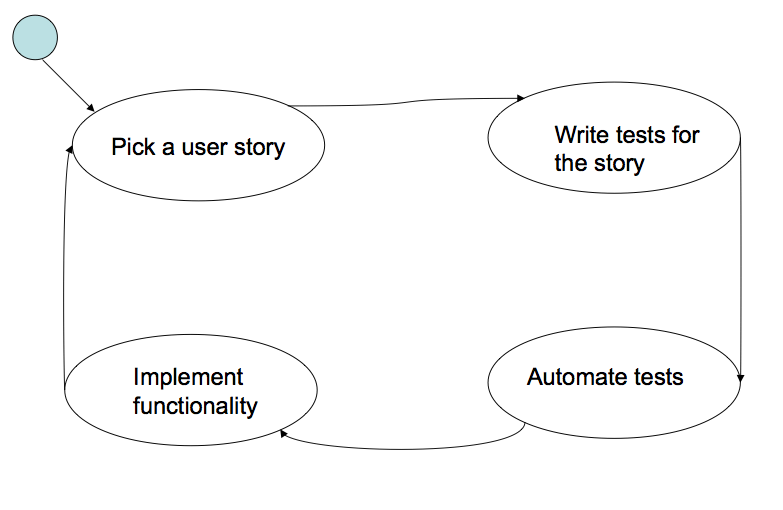
\includegraphics{Forelesning 12/img/1.png}
\caption{}
\end{figure}

\subsubsection{Valg av user story}

Prioritering i forhold til forretningsverdi og teknisk risiko, om der
ikke foreligger en prioritering fra før.

Leverage = (Business value - Tech. risk) / Tech. risk

Ellers vil en på dette stadiet ha en god innsikt i brukerens krav og
behov gjennom uformelle diskusjoner o.l.

\subsubsection{Skrive tester for historien}

Sitt sammen med kunde og beskriv de viktigste scenarioer for denne
user-storien. Kom så til en avtale om hva som behøves implementert for å
kunne realisere hvert scenario.

Resultatene fra disse samtalene vil være et sett godt definerte tester
og forventede resultater (akseptansekriterier). Sistnevnte inkluderer
forventede resultater og systemets forventede tilstand etter endt test.

\subsubsection{Automasjon av testene}

Tabellrepresentasjon (ala (FITNESS){[}\#fitness{]} brukes mye. Det en da
trenger er:

\begin{itemize}
\item
  Funksjonens ID
\item
  Input-parametre
\item
  Forventede resultater
\end{itemize}
\subsection{Pro TDD}

\begin{itemize}
\item
  Forbedre refaktorering. Endre strukturen, ikke oppførselen
\item
  Gjør ditt beste for å oppnå høy dekningsgrad på testene (Strive for
  high test coverage)
\item
  Skriv små snutter av både kode og tester
\item
  Fokus på manglende funksjonalitet- skriv tester som feiler
\end{itemize}
\section{Definisjoner}

\textbf{Hendelse} (Forelesning 15/15.4)

\begin{itemize}
\item
  Enhvert tilfelle som systemet er ment å svare på.
\end{itemize}
\textbf{Meta-data} (Forelesning 09/9-2)

\begin{itemize}
\item
  Data relatert til komponenter, \emph{men er ikke kode}.
\end{itemize}
\textbf{Retrospector} (Forelesning 09/9-2)

\begin{itemize}
\item
  Et verkøty som registrerer testing og utføringshistorien til en
  komponent. Denne informasjonen lagres som
  \href{\#componentmeta-data}{meta-data}.
\end{itemize}
\textbf{Retro-component} (Forelesning 09/9-2)

\begin{itemize}
\item
  Programvare med en retrospector.
\end{itemize}
\textbf{Intern robusthet} (Forelesning 09/9-2)

\begin{itemize}
\item
  Komponentens evne til å håndtere feil i komponenter eller miljø. For å
  teste dette behøver en wrappere, feilinjeksjon, m.m. Intern robusthet
  vil være viktigst i de komponenter som kun er synlige inne i systemets
  grenser.
\end{itemize}
\textbf{Ekster robusthet} (Forelesning 09/9-2)

\begin{itemize}
\item
  Komponentens evne til å håndtere feil i inndata. Her behøver en kun
  komponenten ``as is''. Ekstern robusthet er viktig hvor komponenten er
  en del av brukergrensesnittet.
\end{itemize}
\textbf{Wrapper} (Forelesning 09/9-2)

\begin{itemize}
\item
  En implementasjon som definerer den funksjonaliteten vi ønsker tilgang
  til. Dette kan, men behøver ikke, være et objekt.
\item
  ``Wrapper''-klassen tilbyr et objektgrensesnitt samt metoder som
  håndterer impementasjonen. Istedet for å kalle på en metode i
  implementasjonen direkte, kaller klienten metoden via wrapperen som
  videre aksesserer implementasjonen.
\end{itemize}
\textbf{Bayes' teorem} (Forelesning 09/9-2)

\begin{itemize}
\item
  \texttt{P(B\textbar{}A) = P(A\textbar{}B) P(B)}
\end{itemize}
\textbf{Domene} (Forelesning 06/6.1)

\begin{itemize}
\item
  Et sett input-verdier hvor programmet ufører den samme utregningen for
  hvert nummer i settet. Vi ønsker å definere domene slik at programmet
  utfører ulike utregninger på nærliggende domener.
\end{itemize}
\textbf{Modell} (Forelesning 03/3 - Traceability, Testability)

\begin{itemize}
\item
  En abstraksjon av virkeligheten.
\end{itemize}
\textbf{Metamodell} (Forelesning 03/3 - Traceability, Testability)

\begin{itemize}
\item
  Modeller av modeller, en videre abstraksjon av virkeligheten som
  belyser egenskaper ved modellen.
\end{itemize}
\textbf{Testability} (Forelesning 03/3 - Traceability, Testability)

\begin{itemize}
\item
  The capability of the software product to enable modified software to
  be validated. (ISO 9126)
\end{itemize}
\textbf{From test to requirement} (Forelesning 02/2.1-2)

\begin{itemize}
\item
  Why do we need this test?
\end{itemize}
\textbf{From requirement to test} (Forelesning 02/2.1-2)

\begin{itemize}
\item
  Where is this requirement tested?
\end{itemize}
\textbf{Formålet med smidig utvikling} (Forelesning 02/2.1-2)

\begin{itemize}
\item
  utsette så mange avgjørelser så mye som mulig for å øke graden av
  frihet til ens forståelse er god nok. Øke forståelse ved å ta med folk
  som kan noe om lignende problemer.
\end{itemize}
\textbf{Deskriptive statements} (Forelesning 02/2.1-2)

\begin{itemize}
\item
  Observasjon av den virkelige verden, uavhengig av systemets oppførsel.
  Eks: Er togdørene åpne er de ikke lukket.
\end{itemize}
\textbf{Preskriptive statements} (Forelesning 02/2.1-2)

\begin{itemize}
\item
  Beskriver ønskelige egenskaper om systemet, som kan stemme avhengig av
  hvordan systemet oppfører seg.
\item
  Slik tilstanden oppfattes av systemet.
\item
  Enforced \textbf{solely} by the software-to-be. Formulert av fenomen
  som deles mellom programvare og miljø.
\item
  Programvare forstår dette via sensorer, handler med aktuatorer.
\end{itemize}
\textbf{\emph{Ontologi}} (Forelesning 02/2.3)

\begin{itemize}
\item
  Thesaurus (Domenekonsepter som entiteter, termer og hendelser) +
  inferensregler (Relasjoner, attributter og aksiomer).
\end{itemize}
\textbf{\emph{Boilerplate}} (Forelesning 02/2.3)

\begin{itemize}
\item
  En basis for sjekking av krav. Enkle å forstå for interessenter i
  forhold til mer formelle representasjoner.
\end{itemize}
\textbf{Aktør} (Forelesning 11/11.2)

\begin{itemize}
\item
  Eksterne parter som interagerer med systemet. Har en \emph{rolle}
  (tilsvarer \emph{ikke} jobbtittel). Denne rollen responderer til
  systemets spørringer.
\item
  En aktør behøver ikke være en person -- det kan være et system eller
  et subsystem.
\end{itemize}
\textbf{Use Case} (Forelesning 11/11.2)

\begin{itemize}
\item
  En sekvens av handlinger som systemet utfører som resulterer i et
  observerbart resultat av en verdi til en aktør-
\end{itemize}
\textbf{Use Case Model} (Forelesning 11/11.2)

\begin{itemize}
\item
  Inneholder en aktørliste, pakker, diagrammer, use-cases og views.
\item
  Inkluderer strukturererte use-case-beskrivelse som er forankret i
  veldefinerte konsepter begrenset av krav og omfang.
\end{itemize}
\textbf{Use case map} (Forelesning 11/11.2)

\begin{itemize}
\item
  En visuell representasjon av et systems krav ved å bruke er presist
  definert sett av symboler for ansvar, systemkomponenter og sekvenser.
\item
  Lenker sammen oppførsel og struktur på en eksplisitt og visuell måte.
\end{itemize}
\textbf{Use case map path} (Forelesning 11/11.2)

\begin{itemize}
\item
  Arkitekturiske entiteter som beskriver uformell relasjon mellom
  ansvar, som bundet til underliggende organisatoriske strukturer av
  abstrakte komponenter.
\item
  Brukes for å skape en kobling mellom krav og detaljert design.
\end{itemize}
\textbf{Kompletthetskriterier} (Forelesning 05/5 - Test vs Inspection)

\begin{itemize}
\item
  SOMETHING
\end{itemize}
\textbf{Fixtures} (Forelesning 12/12.1)

\begin{itemize}
\item
  Sett med objekter som vi har instansiert for å bruk i testene
\item
  En fixture er et stykke kode vi ønsker å teste
\end{itemize}
\textbf{Test doubles} (Forelesning 12/12.1)

\begin{itemize}
\item
  \emph{``Object stand-in''}. Ser ekte ut fra utsiden, men kjører
  fortere og er enklere å utvikle og vedlikeholde.
\item
  Brukes for to typer testing: tilstandsbasert testing og
  interaksjonsbasert testing.
\item
  \emph{stubs}, \emph{fakes}, \emph{mocks}.
\end{itemize}
\textbf{Tilstandsbasert testing} (Forelesning 12/12.1)

\begin{itemize}
\item
  Brukes for å teste hvor godt et objekt lytter. Responderes det korrekt
  på input?
\end{itemize}
\textbf{Interaksjonsbasert testing} (Forelesning 12/12.1)

\begin{itemize}
\item
  Brukes for å verifisere hvordan et objekt snakker med sine
  kollaboratører.
\end{itemize}
